%% ----------------ATENCIÓ-----------------------
%% Aquest document està preparat per codificació 
%% UTF-8. Si es llegeix amb un editor 
%% preparat per una altra codificació alguns 
%% caràcters no es veuran correctament.
%%---------------------------------------------- 
%%
%% Aquest document vos pot servir de base per la
%% realització de la memòria del treball final de
%% grau. Es recomana seguir els consells que 
%% apareixen en els diferents comentaris del 
%% document. Convindrà mantenir l'estructura
%% d'aquest exemple i introduir canvis sols 
%% allà on s'indiqui.
%%
%%-----------------------------------------------
%%
%% La plantilla preparada per a la realització de
%% la memòria és la classe LaTeX TFGEPSUIB.cls
%% que es fonamenta en la classe memoir. Aquesta
%% emula alguns `packages` que, per tant, no serà
%% necessari incloure dins el vostre document. El
%% manual de memoir explica quins són aquests
%% paquets (per exemple booktabs, array, tabluarx). 
%% Per altra banda, TFGEPSUIB també carrega 
%% automàticament els paquets, fontenc, xcolor, 
%% graphicx i microtype.
%%
%%-----------------------------------------
%% Opcions de la classe TFGEPSUIB:
%%
%% Per defecte, la classe TFGEPSUIB suposa
%% que la memòria es redactarà en català i que 
%% els estudis són els de Grau en Enginyeria
%% telemàtica. 
%%
%% Si preferiu utilitzar el castellà o anglés
%% per a la redacció de la memòria podeu
%% fer-ho indicant-ho a les opcions.
%\documentclass[catalan]{TFGEPSUIB}
\documentclass[spanish,GINF]{TFGEPSUIB}
%%
%% Per indicar quins són els estudis pels quals
%% es redacta la memòria heu d'incloure una de
%% les següents opcions:
%%
%% GTEL - Grau en Enginyeria Telemàtica
%% GMAT - Grau de Matemàtiques
%% GINF - Grau d'Enginyeria Informàtica
%% GEDI - Grau d'Enginyeria d'Edificació
%% GELE - Grau d'Eng. Elec. Ind. i Automàtica
%% GAGR - Grau en Eng. Agroali. i del Medi Rural
%%
%% Per escriure la memòria en castellà pels estudis
%% de matemàtiques, la línia inicial serà
%\documentclass[spanish,GMAT]{TFGEPSUIB}
%%------------------------------------------

% Per incloure expressions matemàtiques en
% el document és recomanable usar els paquets
%\usepackage{amsmath,mathtools} 

% Per incloure fragments de codi hi ha diferents
% paquets disponibles. Triau el que vos sigui 
% més convenient, per exemple listings. 
%\usepackage{listings} 

% Amb tcolorbox podeu definir caixes per llistats,
% teoremes, exemples, ...
%\usepackage{tcolorbox}

% Si voleu que les referències bibliogràfiques
% apareguin amb el format "autor-any" en comptes 
% de "número" heu d'usar el paquet natbib.
%\usepackage[round,colon,sort&compress]{natbib} 

% En general, la documentació tècnica pot
% incloure molts acrònims. Per això es recomana
% usar el següent paquet. Consultau el corresponent
% manual per saber com s'usa.
\usepackage[printonlyused]{acronym}

% Les diferents unitats de mesura tenen un
% format estàndard de representació que convé
% respectar. Per això s'usa el paquet `siunitx`.
% També permet representar nombres en notació
% científica i alinear correctament els valors 
% numèrics a les taules. Pegau una ullada al 
% manual. Si no voleu usar-lo comentau la línia. 
\usepackage{siunitx}

% Com que és convenient que el paquet hyperref
% sigui un dels darrers en carregar-se, si voleu 
% afegir nous paquets, feis-ho a continuació.
%\usepackage{}

% El paquet "hyperref" crea enllaços automàticament 
% dins el document. Aquests enllaços permeten la 
% navegació a través de les diferents referències 
% figures, bibliografia, fórmules, índex, ...
% tant sols assenyalant-los amb el ratolí. 
\usepackage[backref, colorlinks=true, all colors=black]{hyperref}

% Si voleu que els enllaços apareguin en colors diferents,
% eliminau l'opció "all colors=black". 

%----------------------------------------------
% Dades de la Portada amb els valors adequats
% La portada inclou informació del estudis,
% títol del projecte, autor(s) del projecte,
% tutor(s) i data. 
%
% Els estudis ja s'han definit amb la opció
% corresponent, però si el projecte
% és d'uns altres estudis no definits a les
% opcions, com són, per exemple, els dels plans
% anteriors, sempre podeu usar la comanda \estudis
% per definir-los.
% Per exemple, per l'enginyeria tècnica en 
% telemàtica podeu usar:
%\estudis{Enginyeria Tècnica en Telecomunicacions, especialitat Telemàtica}

%\estudis{Qualsevol grau de l'EPS}

% Aquí podeu posar el títol de la vostra memòria
\title{Red Inteligente Segura de los Grandes Hospitales de Mallorca}

% Nom de l'autor del TFG.
\author{Victor Canelo Galera}

% La comanda \tutor mostra el nom del director
% a la portada interior. Si hi ha més d'un tutor
% caldrà fer un petit canvi. Demanau ajuda. 
\tutor{Sebastià Galmes}

% Indicau el curs acadèmic que correspongui.
\date{Año académico 2024-25}

% Indicau les paraules claus del vostre treball.
\paraulesclau{TFG, memoria, \LaTeX}

% Si l'autor no autoritza la publicació del treball
% descomentau la línia següent
%\autorfalse

% Si el tutor no autoritza la publicació del treball
% descomentau la línia següent
%\tutorfalse

%---------------------------------------------------------------------------------------------------------------------------------------------------------------

% Durant l'escriptura de la memòria haureu de 
% compilar-la moltes vegades. Si voleu guanyar
% una mica de temps, podeu dividir el contingut
% en diferents fitxers i compilar-ne sols alguns.
% La comanda següent és la que vos permet
% definir quins compilar i quins no.
%\includeonly{Instruccions,Annexos}

% Quan vulgueu treballar amb tot el document, 
% simplement, comentau la línia anterior.  

\begin{document}

% Recordau haver indicat, títol, autor i tutor
% i no toqueu les línies següents.
\portada
\portadainterior
\frontmatter

% Voleu dedicar i agrair el treball a algú?
% Activau les línies següents i escriu el
% que vulguis dins l'entorn 'agraiments' 
%
\cleartorecto \thispagestyle{empty}
\begin{agraiments}
Gràcies a tots els professors que m'han ajudat a arribar a aquesta fita dels meus estudis.
\end{agraiments}

% A continuació el Sumari
\cleartorecto \tableofcontents

% Si voleu que apareguin una llista de figures
% i taules, activau les línies corresponents
%\cleartorecto \listoffigures
%\cleartorecto \listoftables 

% Si apareixen molts acrònims a la documentació
% convindrà fer-ne una llista. Podeu veure com
% crear-la consultant el fitxer 'Acronims.tex',
% que és el que s'inclou aquí.
\chapter{Acrònims} %Respectau títol del capítol.
%
% Per utilitzar els acrònims es recomana fer un poc 
% de recerca bibliogràfica per entendre com 
% funcionen. Concretament podeu llegir el manual
% que teniu dins el vostre sistema.
% La comanda `texdoc acronym` hauria de mostrar-lo.
%
\begin{acronym}

\acro{AMC}[AMC]{Adaptive Modulation and Coding}

\acro{EPS}[EPS]{Escola Politècnica Superior}

\acro{IP}[IP]{Internet Protocol}

\acro{LTE}[LTE]{Long Term Evolution}

\acro{MIMO}[MIMO]{Multiple-Input Multiple-Output}

\acro{OFDM}[OFDM]{Orthogonal Frequency Division Multiplexing}

\acro{OFDMA}[OFDMA]{Orthogonal Frequency Division Multiple Access}

\acro{RDI}[R+D+I]{Recerca, Desenvolupament i Innovació}

\acro{TCP}[TCP]{Transport Control Protocol}

\acro{TDMA}[TDMA]{Time Division Multiple Access}

\acro{TFG}[TFG]{Treball Final de Grau}


\end{acronym}
 
% Si no usau acrònims, comentau la línia anterior

% En l'arxiu Resum.tex es posarà el resum
% del treball.
%!TeX root=MemoriaTFG.tex

\chapter{Resumen}

En la actualidad, el correcto diseño y la adecuada seguridad de las redes hospitalarias son aspectos críticos para garantizar la continuidad asistencial, 
la privacidad de los datos clínicos y la disponibilidad de los sistemas médicos. Dado que los hospitales manejan información sensible y dispositivos 
vitales que requieren una conectividad estable y protegida, resulta imprescindible implementar infraestructuras de red seguras, segmentadas y adaptadas a las 
particularidades de este entorno. Además, la creciente incorporación de dispositivos médicos (IoMT) aumenta la superficie de exposición y demanda 
estrategias más restrictivas para su protección. \\

En este proyecto se presenta el diseño y simulación de dos redes hospitalarias utilizando Cisco Packet Tracer: una propone una red detallada para el Hospital Son Espases y la otra 
propone una red de interconexión entre los cuatro hospitales más grandes de Mallorca (Son Espases, Hospital de Manacor, Hospital Comarcal de Inca y Son Llàtzer), incorporando diversas medidas de seguridad tanto a 
nivel físico como lógico. La solución propuesta segmenta la red mediante VLANs para aislar los distintos departamentos del hospital y establece políticas de 
seguridad mediante listas de control de acceso (ACLs), además de incluir redundancia tanto a nivel de hardware como a 
nivel de enlace, así como protocolos y servicios de red esenciales como DHCP o NAT. Como elemento diferencial, se ha implementado una subred específica para dispositivos IoMT, configurada con restricciones y medidas de seguridad 
avanzadas que limitan su interacción con el resto de la infraestructura, minimizando así los riesgos asociados a su conectividad.
 

% No toqueu la línia següent 
\mainmatter\pagestyle{ruled}

%%%%%% COS DEL TREBALL %%%%%%%%%%%%

% Una bona pràctica consisteix en dividir
% un document llarg en diferents fragments,
% per exemple per capítols, i incloure aquests
% fragments dins el fitxer principal amb la
% comanda \include. Així, podem escriure la 
% comanda \includeonly{llista fitxers a compilar}
% que ens permetrà processar sols aquella part
% del document que ens interessi.

%!TeX root=MemoriaTFG.tex

\chapter{Introducció}

Els professionals de la comunicació tenen molt clar que \emph{la manera com s'explica una història és tan important com la pròpia historia}. No n'hi ha prou amb el fet de tenir una bona idea, un projecte de negoci extraordinari o uns resultats molt interessants, si no som capaços de presentar-los d'una manera adequada, el més probable és que no arribin a bon port.

\emph{Tant en l'àmbit acadèmic com en el laboral, saber comunicar d'una manera efectiva ens obrirà moltes portes}. En ambdós àmbits, tindrem idees, planejarem projectes o obtindrem resultats que, d'una manera o altra, haurem d'explicar als professors i companys d'una assignatura, als membres d'un tribunal acadèmic, als membres del gabinet tècnic d'una empresa, a un possible client o al nostre cap de secció. De l'\emph{impacte} que produeixi la nostra explicació (oral o escrita) en dependran, entre d'altres,
\begin{itemize}
 \item \emph{en l'àmbit acadèmic}: l'acceptació a tràmit i la valoració d'una tesi, l'obtenció de finançament per realitzar un projecte de recerca o la publicació d'un article en un congrés o en una revista i,
 \item \emph{en l'àmbit laboral}: l'aprovació del pressupost per a un projecte de part de la gerència de l'empresa, la signatura d'un contracte de serveis amb una altra empresa, la renovació del nostre contracte laboral, l'obtenció de subvencions per engegar un projecte de \acsu{RDI} o la nostra posició de lideratge.
\end{itemize}
Així doncs, atesa la seva rellevància per al nostre desenvolupament personal i professional, és important que ens esforcem per millorar les nostres capacitats de redacció i presentació de treballs científics i tecnològics.

El camp de la comunicació científico-tecnològica és molt ampli, amb tendències teòriques molt diverses, quantitats ingents de llibres i articles sobre el tema i, fins i tot, programes universitaris de grau i de postgrau. Per raons òbvies, doncs, aquest document no pretén abastar tot aquest camp, ni tan sols substituir la lectura d'altres referències bibliogràfiques molt recomanables. Només pretén fer una breu introducció a les habilitats que s'han de treballar per tal de ser un bon comunicador en qualsevol de les activitats acadèmiques i professionals pròpies d'un científic o d'un enginyer. La millora de les nostres habilitats de comunicació es traduirà en la millora dels nostres projectes i de les organitzacions en què treballem i, potser més important, en la millora de la nostra satisfacció personal i de les nostres carreres acadèmiques i professionals.

En l'àmbit universitari el \acf{TFG} constitueix una part important dels estudis de grau. L'objectiu fonamental d'aquest treball, tot i que sovint requereix estudis addicionals en un camp determinat, és que els estudiants apliquin els coneixements, les habilitats i les competències adquirides en els seus estudis de grau a la resolució d'un problema aplicat. Atesa l'obligatorietat de la presentació d'una proposta i d'una memòria de \acf{TFG} i de la defensa oral d'aquest treball davant un tribunal acadèmic, centrarem els continguts d'aquest manual en la introducció dels principis bàsics per a la redacció i presentació d'aquest tipus de treballs. Tanmateix, intentarem que les recomanacions siguin prou generals com perquè puguin ser fàcilment esteses a altres activitats de comunicació científico-tecnològica.

Dedicarem el capítol \ref{instruccions} a fer una petita descripció de les instruccions generals i l'itinerari a seguir per a la realització del \ac{TFG}. Als capítols \ref{proposta} i \ref{memoria} ens centrarem, respectivament, en els aspectes formals de la redacció de la proposta i de la memòria del \ac{TFG}. En el capítol \ref{presentació} descriurem els principis bàsics i les bones pràctiques per a la realització de la defensa oral del \ac{TFG} davant del tribunal. Acabarem amb una secció que recollirà les conclusions més importants d'aquest manual.


%!TeX root=MemoriaTFG.tex

\chapter{Instruccions generals i itinerari del Treball Final de Grau }\label{instruccions}
\begin{figure}
\centering
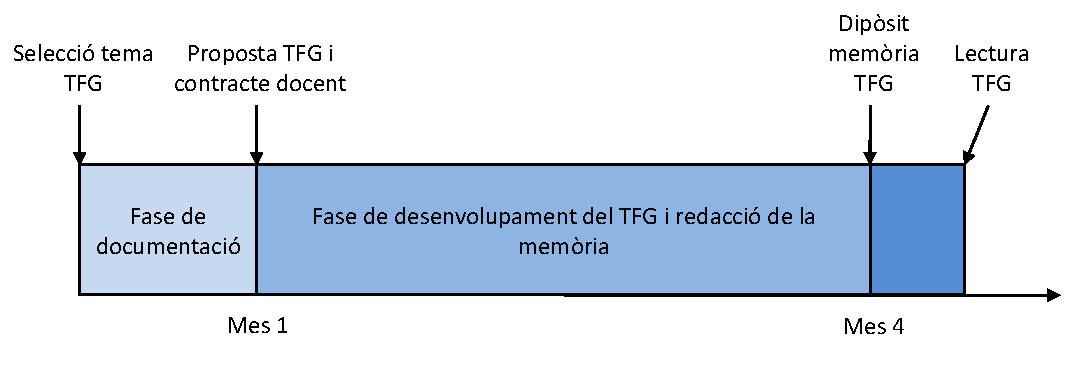
\includegraphics[width=\linewidth]{Itinerari_TFG}
\caption{\label{fig:itinerari}Itinerari del Treball Final de Grau}
\end{figure}

\section{Inici del Treball Final de Grau}

Com a norma general, tal com apareix reflectit en els plans d'estudis de gairebé totes les titulacions de grau, el \ac{TFG} s'hauria de realitzar en el segon semestre de quart curs. Tanmateix, tot i que aquestes s'agrupen en cursos i semestres, els estudis universitaris s'estructuren en assignatures. Així doncs, atesa la naturalesa integradora del \ac{TFG}, la recomanació general seria que abans de començar a realitzar el \ac{TFG} haguéssim aprovat la major part de les assignatures troncals i obligatòries del grau. De fet, l'ideal seria que només ens manquessin les assignatures que en el pla d'estudis corresponent es cursen simultàniament amb el \ac{TFG}.

\section{Selecció del tema de Treball Final de Grau}

Una de les vies més habituals per escollir el tema de \ac{TFG} és a través de l'apartat corresponent de la web de l'\acf{EPS}. En aquest cas, després de revisar les propostes realitzades pels diferents professors o grups de recerca involucrats en la docència de l'\ac{EPS}, escollirem les que més ens interessin i contactarem amb els professors responsables. Si algun dels professors encara no té el tema assignat i ens accepta, començarem a treballar en la fase de documentació i en la preparació de la proposta.

Existeixen altres possibilitats a l'hora d'escollir un tema de \ac{TFG}. Per exemple, podem realitzar el \ac{TFG} en una empresa del sector. En aquest cas és important que contactem amb un professor de l'\ac{EPS} que vulgui realitzar les tasques de supervisió i que pertanyi a un àrea de coneixement propera als continguts a tractar en el \ac{TFG}, d'aquesta manera ens assegurarem que la proposta de \ac{TFG} i el camp que aquesta cobreix compleixen amb els estàndards habituals a la nostra titulació. En cas de dubte, el més convenient és contactar amb el cap d'estudis de la titulació corresponent que segur que ens orientarà i ens proporcionarà la informació necessària.

Val a dir que el \ac{TFG} també es pot realitzar en una universitat amb la que s'hagin establert convenis de convalidació (programes Sèneca, Erasmus, Averroes, \ldots). Tanmateix, en aquest cas haurem de seguir els procediments administratius establerts en aquesta altra universitat.

\section{Preparació de la proposta i contracte docent}

Un cop escollit el tema de \ac{TFG} començarem a treballar en la fase de documentació i, d'acord amb el nostre supervisor, prepararem la proposta de \ac{TFG}. Per a la redacció d'aquesta proposta convé seguir les indicacions descrites al capítol \ref{proposta} i és recomanable que aquesta fase de documentació i preparació de la proposta de \ac{TFG}, tal com es mostra a la Fig. \ref{fig:itinerari}, no s'allargui més enllà d'un mes. Sobre la proposta de \ac{TFG} és sobre la que estudiant i professor signaran el contracte docent. En aquest contracte s'establiran els compromisos del professor quant a seguiment i supervisió del projecte i els de l'estudiant quant a dedicació i termini de presentació. La proposta de \ac{TFG} i el contracte docent, signat tant per l'alumne com pel professor, seran lliurats als serveis administratius on l'\ac{EPS} signarà el compromís de disponibilitat de medis materials genèrics i de formalització d'un tribunal de \ac{TFG} adient.

\section{Desenvolupament del Treball Final de Grau}

Un cop aprovada la proposta de \ac{TFG} ens dedicarem a la realització del \ac{TFG} i a la redacció de la memòria sota la supervisió del director i seguint les condicions estipulades en el contracte docent. Per a la redacció de la memòria convé seguir les indicacions descrites al capítol \ref{memoria}. És recomanable que aquesta fase de desenvolupament i redacció del treball, tal com ens mostra la Fig. \ref{fig:itinerari}, no superi els quatre mesos.

\section{Dipòsit de la memòria}

Una vegada acabada la seva redacció, i amb el vist-i-plau del nostre supervisor, dipositarem la memòria del \ac{TFG} a secretaria seguint les indicacions de la normativa de \acsp{TFG} de l'\ac{EPS}.

\section{Preparació de la presentació}

Finalment només ens quedarà preparar la presentació del \ac{TFG} per tal de fer-ne la defensa oral davant el tribunal. Per a la preparació d'aquesta presentació convé seguir les indicacions del capítol \ref{presentació}.

% !TEX root=ManualTFG.tex

\chapter{La proposta de treball de final de grau}\label{proposta}

\section{Principis bàsics}
En un treball de final de grau ben planificat, la proposta de \ac{TFG} constituirà el primer document formal relatiu al projecte. A més, especialment amb la introducció del contracte docent relatiu al \ac{TFG}, la proposta assoleix una importància cabdal ja que aquest és el document sobre el qual estudiant, director i \ac{EPS} adquireixen compromisos respecte de la duració màxima del treball, tasques de supervisió, disponibilitat de materials, \ldots

La redacció d'una proposta ben definida i consensuada entre director i alumne suposa avantatges importants com, per exemple:
\begin{itemize}
\item Garanties de que, abans d'iniciar el desenvolupament del \ac{TFG}, l'alumne comprèn perfectament el problema que es vol abordar i és capaç de contextualitzar-lo, entenent com la temàtica del seu \ac{TFG} lliga amb la resta de coneixements de l'àrea.

\item Disponibilitat d'una descripció precisa dels objectius del \ac{TFG} i d'una estimació dels resultats que se n'esperen.

\item Visualització del full de ruta del \ac{TFG} que ha de permetre, tant al director com a l'alumne, l'avaluació del progrés en l'execució del projecte i en l'assoliment dels objectius.
\end{itemize}

En la major part dels casos, la proposta formal d'un \ac{TFG} es redactarà a partir d'una proposta de tema provinent d'un professor o d'un grup de recerca. Aquesta proposta de tema descriurà breument el context del treball, el problema adreçat i els objectius que s'intenten assolir. A més, hauria de proporcionar les referències i eines bàsiques a utilitzar i explicitar, també, els coneixements previs i habilitats recomanades per poder dur a terme el \ac{TFG}. El més desitjable seria que totes les propostes de temes de \ac{TFG} es fessin públiques a través de la web de l'\ac{EPS}, tanmateix és probable que també n'apareguin als taulers d'anuncis, portes dels laboratoris de recerca o les portes dels despatxos dels professors. És responsabilitat dels alumnes estar atents a la publicació d'aquests anuncis.

Es pot donar el cas d'alumnes que prefereixin realitzar el \ac{TFG} en una empresa o alumnes que estiguin especialment interessats en un àrea de coneixement concreta i ells mateixos vulguin proposar un tema de \ac{TFG}. En qualsevol d'aquests casos és important que trobin un supervisor i que discuteixin amb ell la preparació de la proposta formal de \ac{TFG}. En el cas de \ac{TFG}s desenvolupats en empreses serà important també comptar amb el vist-i-plau del director/tutor dintre de l'empresa.

El més habitual serà que l'alumne interessat en una proposta de tema de \ac{TFG} comenci llegint les referències bàsiques subministrades per tal d'assolir uns coneixements bàsics sobre el context general del tema proposat i poder plantejar el problema que es vol abordar i els objectius concrets que es persegueixen. Això, comptant amb el suport del supervisor del \ac{TFG}, ha de permetre passar a l'etapa de redacció de la proposta formal del \ac{TFG}. L'elaboració de la proposta pot implicar l'estudi de conceptes que no s'han cobert en els estudis de grau, la cerca de referències bibliogràfiques addicionals a les subministrades a la proposta del professor o l'avaluació d'eines \emph{hardware} i/o \emph{software} que no s'havien utilitzat abans.

La transició des de la proposta de tema del professor cap a la proposta formal de \ac{TFG} per part de l'alumne pot servir, també, per adaptar l'enunciat general d'un problema a un enunciat més específic que reculli les inquietuds de l'estudiant. A més, la proposta d'un professor o d'un grup de recerca pot acabar derivant en més d'una proposta de \ac{TFG} si hi ha més d'un alumne interessat en el tema i és possible estructurar-la en diversos \ac{TFG}s.

Finalment, és important recordar que la proposta de \ac{TFG} s'adjuntarà a un contracte docent entre director, alumne i \ac{EPS} i, per tant, ha d'estar consensuada entre les tres parts.


\section{La proposta de tema}

El format de la proposta de tema del professor serà bastant variable ja que dependrà molt del tipus de projecte concret a desenvolupar i també de l'\emph{estil} de cada professor. En qualsevol cas hauria de contenir informació suficient per a que l'alumne pugui tenir una idea prou clara de en què consisteix el projecte i quins objectius es persegueixen, de quins coneixements li faran falta per afrontar-ho i de quines són les referències bàsiques del tema, que poden servir com a punt de partida per entendre altres referències necessàries per redactar la proposta de \ac{TFG}.

Així, doncs, alguns elements importants que haurien de quedar reflectits a la proposta de tema són:
\begin{itemize}
\item Contextualització: La proposta de tema hauria d'incloure una breu introducció al context del \ac{TFG}, però suficientment detallada per facilitar què l'alumne pugui relacionar la feina a fer amb els coneixements adquirits al llarg dels estudis grau.
\item Definició d'objectius: S'haurien d'explicitar els objectius que es perseguiran en el projecte. El grau de concreció dels objectius dependrà del projecte en si: a vegades la proposta de tema ja suggerirà els resultats concrets que es pretén obtenir i en altres ocasions serà feina de l'alumne definir els objectius concrets del seu \ac{TFG}.
\item Bibliografia: A l'hora de proporcionar una llista de referències bibliogràfiques bàsiques s'ha de tenir en compta el nivell de coneixements dels alumnes potencialment interessats
    en el tema de \ac{TFG}. És molt probable que aquesta bibliografia bàsica estigui principalment composta de capítols de llibres i articles introductoris publicats en revistes i congressos.
\item Pre-requisits: La proposta de tema de \ac{TFG} també hauria d'especificar si el \ac{TFG} té pre-requisits en forma d'assignatures que és necessari haver cursat (o estar cursant), habilitats (e.g. programació de baix nivell, càlcul matemàtic) o interessos particulars dels alumnes.
\end{itemize}

La transició des de proposta de tema publicada per un professor o per un grup de recerca cap a la proposta de \ac{TFG} que ha de redactar l'estudiant, amb el suport del seu supervisor, és previsible que impliqui les passes següents:
\begin{itemize}
\item Immersió en el tema: L'alumne haurà de ser capaç de relacionar el tema del \ac{TFG} amb les assignatures que ha cursat durant els seus estudis de grau. Aquest procés ha d'ajudar a l'alumne a prendre consciència de quins coneixements bàsics li faran falta per dur a terme el \ac{TFG}. La bibliografia bàsica proporcionada a la proposta de tema ha de servir per a que l'alumne adquireixi els coneixements fonamentals per contextualitzar el seu treball.
\item Definició d'objectiu: Un cop assimilats els continguts de les referències introductòries s'ha de ser capaç de definir de manera ben concreta els objectius del \ac{TFG}. Per això pot ser necessària la consulta d'altres referències més especialitzades i/o la discussió d'alguns aspectes del treball amb el supervisor. Aquesta definició d'objectius també ha de servir, si és el cas, per incorporar a la proposta els interessos personals del projectista.
\item Programació temporal: Tenir objectius ben delimitats i ser conscients dels coneixements necessaris per dur-los a terme ha de permetre a l'alumne fer una programació temporal realista del \ac{TFG}. Serà important comprovar que aquesta programació temporal s'ajusta a la càrrega de feina que s'havia previst a la proposta de tema i a la càrrega en crèdits ECTS del \ac{TFG}. Si aquest no és el cas, serà necessari tornar a avaluar els objectius del projecte per determinar si aquests s'han d'ampliar o reduir. A l'hora de fer aquesta programació temporal és fonamental que el projectista tingui en compte la càrrega de feina addicional al \ac{TFG} (assignatures, pràctiques en empresa, \ldots). Els diagrames de PERT o GANT són eines útils per realitzar aquesta programació temporal.
\end{itemize}
Com ja s'ha mencionat abans, la proposta de tema pot donar lloc a més d'una proposta de \ac{TFG} si, per exemple, hi ha més d'un alumne interessat en el tema proposat. En aquest cas serà
responsabilitat del supervisor verificar que les diferents propostes, encara que parteixin d'un \emph{background} comú, tenen objectius concrets ben diferenciats.

\section{Estructura de la proposta de Treball Final de Grau}
En general l'estructura de la proposta de \ac{TFG} inclourà:
\begin{itemize}
\item \emph{Títol}: El títol ha de descriure de la manera més precisa possible el treball a realitzar. Aquest títol no ha de coincidir necessàriament amb el títol definitiu que apareixerà a la memòria.
\item \emph{Paraules clau}: La llista de paraules clau ha d'incloure els conceptes fonamentals que formen la base del \ac{TFG}. En cas de que eventualment s'arribi a disposar d'una base de dades de \ac{TFG}s, aquesta llista serà molt útil a l'hora de fer-hi cerques en funció dels temes tractats.
\item \emph{Context}: Aquesta secció ha de servir per situar el \ac{TFG} dins una determinada àrea de coneixement, per fer una descripció concisa sobre l'estat de l'art del tema sobre el que tractarà el \ac{TFG} i per aclarir els motius que han portat a la realització d'aquest treball. Hauria de servir, també, per introduir el plantejament general del problema que es pretén abordar. Els conceptes clau del projecte han d'aparèixer en aquesta secció definits de manera clara per tal de resoldre possibles ambigüitats i malentesos entre alumne i supervisor. És previsible que aquesta secció, juntament amb la dedicada als objectius, constitueixin la base del primer capítol de la memòria del \ac{TFG}.
\item \emph{Objectius}: En els objectius s'han de concretar les fites del treball tot indicant les qüestions específiques adreçades en el \ac{TFG} i els mètodes que s'empraran per donar-hi resposta. És important que siguin objectius mesurables, és a dir, que el seu assoliment sigui constatable.
\item \emph{Programació temporal}: La programació temporal descriurà el ritme i ordre en que s'han d'anar realitzant les diferents activitats. El nivell de detall de la planificació dependrà del que acordin alumne i supervisor quant a la periodicitat de les reunions des supervisió.
\item \emph{Eines}: Aquí s'explicitaran aquelles eines \emph{hardware} i/o \emph{software} que es faran servir per dur a terme el \ac{TFG}.
\item \emph{Bibliografia}. La bibliografia inclourà totes les referències bibliogràfiques rellevants en la redacció de la proposta de \ac{TFG}, tant les proporcionades en la proposta de tema com aquelles que s'hagin pogut descobrir durant els processos de documentació i redacció dels antecedents i objectius de la proposta final.
\end{itemize}

% !TEX root=MemoriaTFG.tex

\chapter{La memòria del treball de final de grau}\label{memoria}

\section{Principis bàsics}

\emph{Què és el que fa que una memòria de \ac{TFG} sigui bona?} Òbviament, la resposta a aquesta pregunta pot ser molt complexa, però hi ha molts autors (vegeu, per exemple, \cite{Perelman01,Malvar08} i els treballs que aquests referencien) que coincideixen en que un informe tècnic o científic ha de reunir les qualitats següents:
\begin{itemize}
   \item \emph{precisió}: aquesta qualitat es fonamenta en tres aspectes complementaris:
   \begin{enumerate}

   \item \emph{precisió del document}, que fa referència a que aquest s'ha de concentrar de forma precisa en el tema que el defineix i n'ha de fer un tractament correcte, basat en evidències científicament demostrables, i amb un nivell de detall apropiat, ni massa general ni excessivament restringit.

   \item \emph{precisió estilística}, que només és possible si es fa un ús curós del llenguatge per tal d'expressar el significat. La precisió en l'ús del llenguatge es fonamenta en el rigor en la utilització de les paraules, en una estructura correcta de les frases i en un ús adequat dels signes de puntuació.

   \item \emph{precisió tècnica}, que es fonamenta en un bon coneixement tècnic de la matèria i del seu vocabulari.
   \end{enumerate}

   \item \emph{concisió}: molt relacionada amb la precisió del document, la concisió es fonamenta en la focalització, és a dir, en la reducció de l'abast del document a l'àmbit estricte de la qüestió que es vol tractar. És molt fàcil caure en la temptació d'incloure en la memòria materials que potser són molt rellevants en el camp en què es desenvolupa el treball, però que no ho són en absolut per comunicar de manera efectiva les aportacions concretes del treball en aquest camp.
       %Com veurem més endavant, la definició precisa i detallada de l'índex de la memòria és una de les estratègies més útils per controlar la longitud i l'abast del document. També és important identificar i eliminar els materials (frases, paràgrafs, seccions, \ldots) que no són necessaris per recolzar o evidenciar les nostres aportacions. Les figures i les taules solen contribuir a la concisió del document perquè redueixen la quantitat de prosa necessària per descriure objectes i processos, resumeixen dades i serveixen per demostrar relacions.
%
   \item \emph{claredat}: aquesta qualitat, que fa referència a la capacitat de qui escriu per facilitar la comprensió del document a qui llegeix, és especialment important en l'escriptura científico-tècnica. Els vocabularis especialitzats, els desenvolupaments matemàtics o els esquemes conceptuals complexos poden dificultar moltíssim la comprensió d'algunes explicacions tècniques, fins i tot quan aquestes han estat redactades per escriptors especialitzats i són processades per lectors experts.

   \item \emph{coherència (organització i estructura)}: un document és coherent si el material que presenta està organitzat de manera lògica i consistent i la seva estructura proporciona al lector un camí fàcil per a la seva comprensió. La coherència es valora de forma molt especial en ciència i tecnologia degut a la inherent complexitat dels temes que es tracten.


   \item \emph{adequació a l'audiència}: és convenient que el document s'adeqüi als objectius que l'autor s'ha marcat a l'hora d'escriure'l, però, sobretot, és molt important que s'adeqüi a les necessitats dels possibles lectors (supervisors, membres del tribunal, altres alumnes que treballin en temes semblants, \ldots) i al context, objectius i convencions (forma i estil) de la institució en què es presenta.
\end{itemize}

Tal com ens recorda H. S. Malvar a \cite{Malvar08}, l'error més freqüent que podem cometre a l'hora d'escriure, especialment en el cas de l'escriptura científica, és no saber posar-nos al lloc del lector. Així doncs, la recomanació fonamental per evitar errors a l'hora d'escriure la memòria és que cada cop que afegim una nova argumentació, una nova figura o una nova taula, pensem en els possibles lectors d'aquesta informació i la revisem per tal de garantir que és precisa, clara, concisa, coherent i adequada a l'audiència.

\section{Bones pràctiques}

\emph{Quines són les millors passes a fer per escriure una bona memòria de \ac{TFG}?} La major part dels treballs de final de grau es desenvolupen en tres etapes, una primera etapa en què es duu a terme una revisió de les referències bibliogràfiques més rellevants sobre el context general i l'àmbit particular del projecte, una segona etapa en què es realitzen estudis analítics, simulacions, implementacions reals, \ldots i, finalment, una tercera etapa en què es redacta la memòria. Tanmateix, aquestes tres etapes no són estrictament consecutives i, habitualment, treuen profit d'una retroalimentació sistemàtica entre elles. En aquesta secció, tot i ser molt conscients d'aquesta interdependència, ens centrarem en l'etapa de redacció de la memòria i presentarem una sèrie de recomanacions a seguir en els processos de \emph{focalització}, \emph{elaboració de l'esbós} i \emph{redacció}.

\subsection{Focalització} Aquest procés aborda de ple les qualitats de precisió del document, concisió i adequació a l'audiència. La focalització consisteix en la reducció de l'abast del document a l'àmbit estricte que el defineix, en la selecció acurada dels temes sobre els que ha de tractar i en l'adequació dels continguts i profunditat de tractament d'aquests a l'audiència concreta a la que es vulgui dirigir. Per focalitzar un document, algunes de les passes que ens podrien servir serien:
\begin{enumerate}
   \item Fer una llista completa dels temes o paraules clau que defineixen el nostre treball.

   \item Si encara no ho hem fet, recórrer a les referències bibliogràfiques que calgui per tal de tenir una visió prou acurada del paper que juga cadascun d'aquests temes en el context general i en l'àmbit particular del tema que ens ocupa.

   \item A partir de la llista de temes i de la informació disponible sobre cadascun d'aquests, respondre a preguntes del tipus:
   \begin{itemize}
          \item És necessari que tracti aquest tema en la memòria?
          \item Es perdran els lectors de la memòria si no tracto aquest aspecte?
          \item Puc deixar de parlar sobre aquest tema sense perjudicar l'objectiu global del meu projecte?
          \item És excessivament general aquest tema o és excessivament específic?
          \item N'hi ha prou amb un tractament general acompanyat de referències bibliogràfiques o seria millor que el lector disposés d'una visió més detallada per tal de poder seguir els raonaments posteriors?
          \item És necessari introduir coneixements previs per poder tractar alguns dels temes de la llista?
   \end{itemize}
   Aquest tipus de preguntes actuaran com a filtres que ens permetran eliminar temes innecessaris, afegir-ne de necessaris o preveure la profunditat amb la que s'ha de tractar cadascun dels temes seleccionats. En haver acabat disposarem d'una bona eina per passar a l'etapa d'elaboració del primer esbós de la memòria.
\end{enumerate}

\subsection{Elaboració de l'esbós} Un cop hem focalitzat l'àmbit estricte del treball i, per tant, disposem de la llista de temes seleccionats i tenim una idea general de la profunditat amb què els volem tractar, una bona manera de facilitar el procés de redacció consisteix en la preparació d'un esbós detallat del nostre treball. Es comença amb una taula de continguts que conté un llistat dels títols provisionals dels capítols, seccions i subseccions que es volen incloure en la primera versió de la memòria. Després, per cadascun dels capítols, seccions i subseccions es redacten una sèrie de frases curtes que descriuen, de forma ordenada, els aspectes clau de tots i cadascun dels continguts que s'hi tractaran i, si es creu convenient, les fonts en les que ens podem recolzar en el procés de redacció. En aquestes etapes continua sent especialment important tenir en ment les qualitats de precisió, concisió i adequació a l'audiència de la nostra proposta, però també hi jugarà un paper especialment rellevant la qualitat de coherència. Paga la pena dedicar temps i esforç en l'elaboració d'aquest primer esbós i revisar-lo tantes vegades com sigui necessari fins a estar-ne totalment convençuts.

Un cop tenim l'esbós provisional del document és el moment de fer-ne una revisió acurada amb l'ajut del nostre supervisor. Aquesta revisió ens hauria de permetre, entre d'altres coses, eliminar el material innecessari, afegir el material o argumentacions que se'ns hagin pogut oblidar i reestructurar els continguts per tal d'incrementar el nivell de coherència del document. És més eficient i menys dolorós prendre aquestes decisions en les fases inicials del procés de redacció, que haver-les de prendre un cop ja s'ha escrit molt de material que al final s'ha de descartar. A partir d'aquest primer esbós ens resultarà més senzill visualitzar l'estructura global de la memòria i saber, en cada moment, quin és l'estat del procés de redacció. Ens permetrà determinar si el treball realitzat (simulacions, implementacions, anàlisis, \ldots), els resultats obtinguts i les referències bibliogràfiques consultades són suficients o si és necessari aprofundir en algun aspecte concret. Ens ajudarà, també, a planificar la nostra feina en funció del temps disponible.

\subsection{Redacció} L'estratègia de redacció a seguir a partir d'aquest primer esbós no ha de ser necessàriament lineal, és a dir, no ha de començar necessàriament amb la redacció del capítol d'introducció i acabar amb la del capítol de conclusions. De fet, tot i que és molt important partir d'una idea molt clara dels continguts del capítol d'introducció, atès que aquest és el que proporciona una visió global del context i l'abast del treball, en la majoria dels casos ens pot resultar més senzill començar amb la redacció dels capítols corresponents al desenvolupament del treball i acabar amb la redacció de la introducció i les conclusions. És l'anomenada estratègia \emph{de dintre cap a fora}.

És molt possible que, a mesura que anem redactant aquesta primera versió de la memòria, també descobrim que és necessari fer addicions, supressions i altres esmenes sobre l'esbós original a fi d'assolir-ne la versió definitiva. En qualsevol cas, atès que les frases curtes que hem utilitzat apunten, de forma ordenada i coherent, els aspectes clau de tots i cadascun dels continguts dels capítols, seccions i subseccions de la memòria, si ens dediquem a desenvolupar-les en forma de paràgrafs, recorrent, sempre que sigui necessari, a l'ajut de figures, taules, desenvolupaments matemàtiques, \ldots, al final obtindrem la primera versió de les diferents parts de la memòria.

La primera versió d'una secció o d'un capítol és la primera passa cap a la versió definitiva, però no ens ha de fer mandra revisar-la i reescriure-la tants cops com sigui necessari per tal de millorar-ne les qualitats de precisió, claredat, concisió, coherència i adequació. Aquest procés de revisió s'ha de fer a consciència, intentant descobrir paraules, frases, taules, figures o, fins i tot, paràgrafs que no contribueixen a que el text sigui més precís o més concís o més clar, procurant, també, millorar l'organització i l'estructura dels diferents elements que conformen el text i, no menys important, mirant d'aconseguir la precisió estilística a través de la correcció ortogràfica i gramatical.

La paraula clau és revisió i, com no podia ser d'altra manera, un cop donem per acabada la primera versió d'un capítol és el moment de que el nostre supervisor també la revisi. Atès que ja havíem mantingut reunions amb el supervisor per discutir l'esbós de la memòria, és poc probable que aquesta revisió suposi canvis substancials en l'estructura general del capítol. Tanmateix, hi pot haver aspectes del treball que només s'hagin tractat de manera més o manco informal i, per tant, la lectura d'aquesta versió pot ser el primer contacte formal del supervisor amb alguns dels plantejaments teòrics o pràctics realitzats per l'alumne. Així doncs, hi ha la possibilitat de que es detectin mancances o errors que suposin el replantejament d'alguns apartats. És molt important que considerem tots els suggeriments que ens faci el supervisor i que els utilitzem per millorar la següent versió de la memòria. Si s'han produït replantejaments d'algunes parts del treball pot ser necessària una segona revisió per part del supervisor.

Quan el supervisor hagi revisat tots els capítols de la memòria i nosaltres hàgim realitzat tots els canvis oportuns, només restarà portar a terme una revisió global de la memòria per tal d'obtenir-ne la versió definitiva.

\section{Estructura del Treball Final de Grau}

Tal com ens recorda el professor Valiente \cite{Valiente96}, organismes internacionals d'estandardització com l'ANSI (\emph{American National Standards Institute}) o la ISO (\emph{International Organization for Standardization}) prescriuen sistemes estàndard per a l'organització dels treballs científics que contenen quatre parts fonamentals: introducció, desenvolupament, resultats i conclusions. Aquestes parts fonamentals d'un treball científic es complementen amb altres components com la portada, la taula de continguts, les llistes de figures, taules i acrònims, el resum, els agraïments, els apèndixs o les referències bibliogràfiques.


\subsection{Portada}

La portada actua com a element de presentació i identificació del \ac{TFG}. Les dades que s'hi han de fer constar poden variar en funció del tipus de treball, però n'hi ha algunes que són fonamentals: títol, autors, directors i, si s'escau, tutors, departament, universitat, títol acadèmic al qual s'opta i data de presentació. Després de la portada s'acostumen a deixar un o més fulls en blanc de cortesia.

El títol és sens dubte una part molt important de la memòria del \ac{TFG}. És el primer lligam que s'estableix entre el \ac{TFG} i el lector i, per tant, s'ha de ser molt curós a l'hora de seleccionar les paraules i les frases que donaran forma al títol. Un bon títol és aquell que descriu el contingut del \ac{TFG} de manera precisa i amb el menor nombre de paraules possible. Una bona estratègia a l'hora d'escriure el títol del \ac{TFG} és partir d'una llista de paraules clau i tractar de trobar quines d'aquestes són fonamentals a l'hora de descriure la nostra aportació i quin ha de ser l'ordre i l'associació entre aquestes paraules clau. Òbviament, a mesura que anem escrivint la memòria podem anar manejant una sèrie d'alternatives que puguin donar lloc a diferents títols i deixar que amb el temps alguna d'elles es vagi imposant sobre les altres.

\subsection{Taula de continguts o Sumari}

La taula de continguts o sumari és un llistat dels títols dels diferents capítols, seccions i subseccions del document amb indicació dels números de pàgina en què apareixen. Per tant, la taula de continguts no només ajuda als lectors a cercar els diferents temes tractats en la memòria, sinó que també serveix com a esbós de l'estructura de la memòria i ofereix una visió general del document als lectors potencials. Òbviament, les taules de continguts més útils es componen de títols de caire descriptiu.

\subsection{Llista de figures}

Els lectors utilitzen la llista de figures per localitzar la informació visual en la memòria. La llista de figures relaciona els títols o llegendes dels recursos visuals (figures, dibuixos, fotografies, \ldots) amb la seva ubicació dintre de la memòria. És important que les llegendes de les figures siguin descriptives i que estiguin numerades de manera consecutiva.

\subsection{Llista de taules}

La llista de taules proporciona les llegendes i la localització de totes les taules que apareixen a la memòria. De la mateixa manera que els títols de figura, els títols o llegendes de les taules s'han de numerar consecutivament en l'ordre en què apareixen al document.

\subsection{Llista d'acrònims}

Hi ha documents que utilitzen una quantitat important de termes nous, o molts acrònims i abreviacions. En aquests casos es pot facilitar la lectura de la memòria si s'inclou una llista de nomenclatura o una llista d'acrònims just després de les llistes de figures i/o taules. Un dels efectes secundaris interessants de les llistes de nomenclatura o d'acrònims és que ajuden a l'autor del document a utilitzar la terminologia d'una manera coherent.

\subsection{Resum}

El resum és una breu declaració, generalment entre 250 i 500 paraules, que proporciona al lector una sinopsi del problema, el mètode, els resultats i les conclusions de la memòria. Els resums s'han de poder llegir de manera totalment independent de les altres parts de la memòria i, per tant, no s'hi han d'utilitzar acrònims sense definir-los i tampoc s'hi han d'utilitzar referències bibliogràfiques. Els resums són extremadament útils per aquelles persones que volen tenir una imatge general del contingut de la memòria abans de llegir el document principal. Atès que hi pot haver lectors potencials que utilitzin el resum per decidir si han de continuar llegint la memòria o no, cal no menystenir la importància d'una bona redacció d'aquest apartat del document. Els resums poden estalviar una immensa quantitat de temps als possibles lectors.

El resum ha d'incloure, com a mínim, els següents elements:
\begin{itemize}\tightlist
   \item Definició abreujada del problema o tema principal del \ac{TFG}.

   \item Exposició del mètode utilitzat per resoldre el problema.

   \item Comentaris sobre els principals resultats, aportacions i possibles aplicacions del treball.

   \item Conclusions més importants del treball
\end{itemize}

\subsection{Agraïments}

A vegades s'inclou una secció d'agraïments en els preliminars de la memòria per tal de donar crèdit a l'assistència rebuda de part de persones i/o institucions. Els supervisors, els tècnics de laboratori o els companys de feina que ens han assessorat o ens han donat suport són, tots ells, candidats a aparèixer al capítol d'agraïments.

\subsection{Introducció}

Si hem decidit utilitzar l'estratègia \emph{de dintre cap a fora}, després de redactar els capítols corresponents al desenvolupament del treball estarem en disposició d'enllestir la redacció de la introducció i les conclusions.

La introducció hauria de servir per donar, de forma descriptiva i fàcil d'entendre, una visió global del context i l'abast del treball. De fet, segons Booth~\emph{et al.}~\cite{Booth08}, el patró comú que cerquen els lectors en qualsevol introducció està format per tres elements:
\begin{itemize}
   \item Contextualització: es tracta d'explicitar el context en el que s'emmarca el treball, d'establir la base comuna de coneixements sobre el tema que es tractarà en la memòria del \ac{TFG}, de garantir que els possibles lectors comparteixen amb l'autor de la memòria el conjunt de factors que els permetran interpretar adequadament els seus enunciats i raonaments.

       El context d'un \ac{TFG} podria ser, per exemple, el món de les xarxes de comunicacions mòbils de quarta generació (4G), amb capes físiques basades en l'ús de múltiples antenes en transmissió i en recepció (\acsu{MIMO} -- \emph{\acl{MIMO}}), tècniques de codificació i modulació adaptatives (\acsu{AMC} -- \emph{\acl{AMC}}) i estratègies d'accés múltiple basades en l'ús de transmissió multiportadora (\acsu{OFDMA} -- \emph{\acl{OFDMA}}). En aquest cas seria adequat parlar sobre l'estat actual del desenvolupament dels estàndards 4G, de les característiques generals de les tecnologies \ac{MIMO}, \ac{AMC} i \acsu{OFDM}/\ac{OFDMA} i de la seva adequació als sistemes 4G. Depenent de l'àmbit d'aplicació del problema a tractar podria ser adequat aprofundir, per exemple, en la descripció de l'estat actual de les xarxes de comunicacions ce\lgem{}lulars i de les característiques de les estacions base i/o de les estacions repetidores o en la descripció de l'estat actual de les xarxes d'àrea local sense fils i de les possibles estratègies de cooperació entre punts d'accés.

   \item Definició del problema: un cop establert el context del treball, és l'hora de definir amb precisió el problema que es tractarà en el \ac{TFG} i de justificar la seva importància dintre del context en el que s'emmarca. Es tracta, també, de proporcionar una visió general, però concisa, dels antecedents del problema, de les publicacions més rellevants sobre el tema, de les virtuts i mancances dels plantejaments i solucions aportades per altres autors.

       Dintre del context de l'exemple anterior, un possible problema a resoldre en un \ac{TFG} podria ser, atesa la necessitat de gestionar els recursos disponibles d'una manera eficient, el de l'assignació òptima de potència, subportadores i modes de transmissió (codificació de canal i modulació) per tal de garantir una taxa de transmissió global màxima amb restriccions sobre la qualitat de servei proporcionada a les aplicacions dels diferents usuaris del sistema.

   \item Resposta al problema: després de definir el problema, el més lògic és presentar al lector de la memòria la nostra proposta per solucionar-lo, els nostres objectius. Es tracta d'explicitar el mètode seleccionat per solucionar el problema plantejat anteriorment, tot justificant aquesta selecció. També pot ser adequat avançar, tot i que de manera concisa, els resultats principals del \ac{TFG} i les possibles conclusions que es desprenen dels resultats obtinguts.

       En el problema de l'exemple anterior, una possible resposta podria consistir en el desenvolupament d'algorismes d'optimització dual, en l'ús de la teoria de jocs o, per posar-ne un altre exemple, en l'ús d'aprenentatge estadístic (\emph{machine learning}). En cadascun d'aquests casos hauríem de justificar la tria feta i, si ens semblés adient, podríem parlar de quins són els resultats que mostrarem al lector en el desenvolupament de la memòria del \ac{TFG}.

\end{itemize}


Avui en dia, tant en la universitat com en l'empresa, és molt habitual que el \ac{TFG} formi part de projectes de recerca més amplis, de manera que pot ser difícil per al lector discernir quan és que l'autor descriu el seu treball personal i quan és que descriu una tasca realitzada per altres membres del grup de recerca. En aquests casos, és molt important que l'autor expliciti el millor possible quin ha estat exactament el seu paper dintre d'aquest projecte general.

Tot i que hi ha autors que no ho recomanen, una manera habitual d'acabar una introducció consisteix en presentar un resum de l'estructura de la memòria, avançant al lector quins són els continguts dels diferents capítols del \ac{TFG}.


\subsection{Desenvolupament}

Aquesta part de la memòria, que es pot estructurar en diversos capítols, tracta sobre la pròpia realització del treball i descriu el que s'ha fet, com s'ha fet, per què s'ha fet d'aquesta manera i no d'una altra, quins materials o eines s'han utilitzat o s'han hagut de desenvolupar, quina metodologia de treball i de validació s'ha seguit, \ldots

L'estructura, organització i contingut d'aquesta part de la memòria depenen en gran mesura del tipus de \ac{TFG}: empírics, estudis de casos, metodològics, teòrics, \ldots\ Tanmateix, el principi bàsic ha de ser proporcionar informació suficient perquè un lector ben informat pugui comprendre, reproduir i verificar els experiments o els desenvolupaments teòrics, tot evitant la simple repetició enciclopèdica de coneixements que es poden trobar a llibres, articles o altres documents de referència. Per exemple, quan la memòria del \ac{TFG} comenci amb els fonaments teòrics del problema plantejat a la introducció, el seu tractament, necessàriament sintètic, ha de mostrar l'elaboració personal de la informació manejada i s'ha de tenir molta cura de no caure en la simple còpia dels autors referenciats. A partir d'aquesta elaboració personal s'entendrà el fil argumental seguit per l'autor a l'hora d'arribar a la resolució del problema plantejat.

\subsection{Resultats i discussió}

Els resultats obtinguts en el \ac{TFG} constitueixen la nostra contribució al coneixement científic. Així, doncs, aquesta part de la memòria ha de descriure tota la informació generada en el desenvolupament del \ac{TFG}. No n'hi haurà prou amb presentar les dades juntament amb les estimacions sobre la seva precisió, també serà necessari interpretar-les i situar-les en context comparant-les amb les obtingudes per altres autors o utilitzant altres mètodes proposats a la literatura.

En els capítols dedicats a la presentació i discussió de resultats és habitual utilitzar figures i taules per tal de mostrar les dades d'una manera efectiva. És important parar molt d'esment en l'elaboració tant de les figures com de les taules i, també, que en el text fem referència explícita als resultats que hi presentem. Si el \ac{TFG} ha produït una gran quantitat de dades potser no cal presentar-les totes en els capítols de resultats i el més adequat és fer-ne una selecció acurada que ens permeti complir amb el propòsit d'extreure'n i fonamentar de forma rigorosa les conclusions del \ac{TFG} i poder-ne fer una presentació adequada als lectors. De fet, si es considera oportú, les dades que no apareguin en aquests capítols de resultats es poden fer avinents als possibles lectors en els apèndixs.

\subsection{Conclusions}

Tot i que el capítol de conclusions d'un \ac{TFG} pot començar amb un resum del context i de la definició del problema i passar després a analitzar la importància del treball realitzat i dels resultats obtinguts, les conclusions no s'han de limitar a tornar exposar el que ja s'ha presentat en els capítols anteriors i, a més, no s'ha de caure en la trampa de repetir el mateix que es va dir a la introducció \cite{Pierson97}. Per tant, el resum del context i de la definició del problema ha de ser molt breu i ens hem de concentrar en la interpretació dels resultats i en la identificació de les nostres contribucions. Les conclusions han de donar resposta a preguntes del tipus: Quines implicacions teòriques i/o pràctiques pot tenir el meu treball? Quin valor afegit suposa aquest treball dintre del corpus de coneixements de la meva disciplina? Què és el que coneixem ara que no se sabia al principi d'aquest treball? Quines mancances i quina utilitat tenen els resultats obtinguts? Què es pot fer a partir d'aquests resultats? Quines portes hem tancat i quines hem deixat obertes? Quines recomanacions podem fer als que vulguin continuar en aquesta línia?

Així, doncs, el capítol de conclusions hauria de:
\begin{itemize}\tightlist
   \item Recordar de manera concisa el context i la definició del problema i dels possibles objectius marcats en la introducció del \ac{TFG}.

   \item Argumentar les principals conclusions del \ac{TFG} i establir les possibles implicacions teòriques i les possibles aplicacions pràctiques dels resultats obtinguts.

   \item Remarcar què és el que ha quedat i el que no ha quedat demostrat en la memòria del \ac{TFG}.

   \item Incloure recomanacions específiques per a futurs treballs relacionats amb el problema tractat en aquesta memòria.
\end{itemize}


\subsection{Apèndixs}

Els apèndixs contenen aquella informació que, tot i ser interessant que estigui en la memòria del \ac{TFG}, per un motiu o altre no és apropiat que aparegui en el cos principal d'aquesta. Els motius poden ser molt diversos però gairebé tots ells estarien relacionats amb la continuïtat del fil conductor de l'argumentació presentada en el cos principal de la memòria. Per exemple, demostracions matemàtiques molt extenses, taules completes de les característiques dels models utilitzats en les simulacions, especificacions tècniques dels components, grans taules de dades o el codi font d'un algorisme, són bons candidats per posar en un apèndix.

\subsection{Referències bibliogràfiques}

El coneixement científic, com qualsevol altre, és acumulatiu i, per tant, és normal que a mesura que anem escrivint la memòria del \ac{TFG} ho fem recolzant-nos en llibres, articles de revista, articles publicats en les actes d'un congrés, treballs inèdits, \ldots d'altres autors. Això és completament ``legal'' (no podrem ser acusats de plagi) sempre que citem de forma adequada les fonts bibliogràfiques utilitzades. Aquestes referències bibliogràfiques serviran, entre d'altres coses, per:
\begin{itemize}\tightlist
   \item donar suport a les nostres reivindicacions o augmentar la credibilitat de les nostres argumentacions,
   \item referenciar els antecedents que ens han portat fins a la feina que presentem en aquest \ac{TFG},
   \item donar exemples de diferents punts de vista sobre un tema determinat,
   \item cridar l'atenció sobre una posició amb la que volem mostrar el nostre acord o desacord, o
   \item destacar una frase o un passatge especialment rellevant tot citant la font original.
\end{itemize}

% !TEX root=MemoriaTFG.tex

\chapter{La presentació del Treball Final de Grau}\label{presentació}

\section{Principis bàsics}
\emph{Què és el que fa que una presentació de \ac{TFG} sigui bona?} L'objectiu de qualsevol presentació és donar a conèixer un determinat missatge fent que l'audiència l'entengui i el recordi \cite{Blair91,Padgett08}. En concret, la presentació del \ac{TFG} ha de permetre a l'alumne sintetitzar el treball que ha estat realitzant durant varis mesos i donar-lo a conèixer als membres del tribunal per tal que aquests puguin determinar fins a quin punt s'han assolit els objectius plantejats.

Les qualitats més rellevants que ha de tenir una presentació tècnica/científica per ser bona són (\cite{Blair91,Padgett08,Arcy88,Rice04}):
\begin{itemize}\tightlist
  \item concisa i precisa: cal identificar les idees clau (objectius i assoliments del treball realitzat) i comunicar-les amb precisió estilística i tècnica.
  \item organitzada i estructurada: una organització acurada i coherent del material a presentar facilita enormement la seva comprensió per part de l'audiència.
  \item adequada a l'audiència i capaç de captar i mantenir la seva atenció: s'ha d'\emph{en\-gan\-xar} l'audiència per tal que entengui millor el que es vol expressar. Per això el missatge s'ha de caracteritzar per la seva:
      \begin{enumerate}\tightlist
        \item claredat
        \item simplicitat
        \item correcció
        \item precisió
      \end{enumerate}
  \item exhaustivament preparada: quan les idees es comuniquen d'una manera pobra no s'obté cap benefici del nostre esforç, ni per part nostra ni per part de l'audiència.
\end{itemize}

L'objectiu serà despertar prou interès en el tribunal com per aconseguir captar veritablement la seva atenció i donar-li a conèixer el problema a resoldre, la solució adoptada i els resultats obtinguts.

\section{Bones pràctiques}
\emph{Quines són les millors passes a fer per preparar una bona presentació de \ac{TFG}?}

\subsection{Les transparències}

        A l'hora de preparar la presentació del \ac{TFG} podem caure en la temptació d'explicar el contingut complet del nostre treball, però l'objectiu ha de ser deixar clars tan sols els punts més importants. Si aquests no són massa nombrosos, serà possible explicar-los de manera clara, mentre que si pretenem mostrar massa idees tan sols aconseguirem confondre l'audiència. Els detalls sobre el treball desenvolupat es troben a la memòria del \ac{TFG} i no s'han d'explicar a la presentació. A l'hora de preparar les explicacions s'ha de tenir present que les nostres idees sempre ens semblen molt més simples a nosaltres que a aquells que encara no les entenen. La clau d'una bona presentació es fonamenta en descriure de manera adequada:
        \begin{itemize}\tightlist
            \item el problema a resoldre: les necessitats del projecte, la seva motivació, explicant la situació i l'entorn en el qual neix, el perquè és necessari
            \item la solució adoptada i els resultats obtinguts
            \item les conclusions del treball i les possibles línies de futur
        \end{itemize}

        És fonamental tenir presents les característiques de l'audiència i proporcionar-li la informació que necessita per tal que pugui entendre la presentació. Sempre és bo començar amb una revisió d'aquells conceptes bàsics que, tot i ser probablement coneguts per l'auditori, facilitaran la comprensió de la presentació. Com a part de la preparació s'han d'avaluar no només els coneixements sinó també els interessos, necessitats i valors de l'audiència (criteris de puntuació del \ac{TFG}).

        Un cop identificats els punts clau que volem deixar clars i les característiques de l'audiència, es realitzarà un esbós del contingut de les transparències. A partir d'aquest esbós es va perfilant l'estructura de la presentació, que ha de seguir un fil argumental lògic i coherent. El contingut de les transparències haurà de marcar en tot moment com es va avançant per aquest fil, evitant que l'audiència es perdi i deixi d'estar atenta. Mantenint sempre aquest propòsit en ment es decideixen els continguts de les transparències, que només inclouran aquelles explicacions necessàries per a poder assolir el nostre objectiu, que no és altre que el de transmetre a l'auditori els punts que hem escollit com a idees clau. Aquells continguts que no siguin imprescindibles per a aconseguir aquesta finalitat no s'inclouran en les transparències.

        Tot i que la normativa estableix una durada màxima de 45 minuts, és recomanable que no excedeixi els 30 o 35 minuts, deixant uns 15 minuts pel torn de preguntes. S'han de redactar les transparències tenint en compte que generalment és recomanable dedicar aproximadament entre dos i tres minuts a cada transparència \cite{Padgett08}. Cal tenir en compte que l'audiència sol perdre l'atenció passats uns 10 o 15 minuts d'activitat similar \cite{Padgett08}. Això significa que el rellotge de l'atenció s'ha de tornar a iniciar en el transcurs de l'exposició oral, i per aconseguir-ho cal donar algun tipus de gir en la presentació, la qual cosa es pot aconseguir, per exemple, amb algun tipus de demostració o de recapitulació.

        En la redacció del text de les transparències es procurarà que tant els títols com les frases siguin directes i curts. Els paràgrafs han de ser breus i l'estil utilitzat ha de ser impersonal i objectiu. A més s'ha de procurar minimitzar el text present a les transparències i s'evitarà sempre copiar paràgrafs complets de la memòria a la presentació. És fonamental assegurar-se de la total correcció ortogràfica i gramatical.

        Les taules, gràfics, diagrames i imatges que mostren el que volem expressar, són eines de comunicació molt valuoses. Cal indicar clarament a l'audiència el que es mostra en aquests elements visuals, mai s'ha de donar per suposat que ja ho sap. D'aquesta manera qui atén les nostres explicacions es beneficia d'escoltar i de veure simultàniament el nostre missatge. Si s'ha de fer alguna demostració de l'aplicació o producte final és convenient gravar-ho en vídeo per tal d'evitar possibles inestabilitats del software o problemes amb els servidors.

        Convé provar les diapositives en el projector i el PC de la sala on es farà la defensa, ja que poden canviar colors, ... També cal confirmar que la mida de lletra és adequada i que els gràfics es visualitzen de manera clara i que són inte\l.ligibles. S'evitaran els colors estridents i els dissenys de diapositiva que restin claredat al contingut de les transparències.

\subsection{L'exposició i la defensa}

        És fonamental preparar-se bé la presentació, explicitant el que s'ha de dir a cada transparència. L'alumne ha de tenir molt clares les explicacions que pretén donar als membres del tribunal, ja que en cas que tingui aspectes confusos mai podrà transmetre'ls amb claredat. És recomanable practicar-la repetides vegades tant tot sol com davant d'altres persones, per tal d'agafar confiança i fluïdesa, així com per ajustar-se al temps disponible. S'evitarà recitar de memòria la presentació, però sí que és bo memoritzar algunes paraules o frases clau per a cada transparència. De totes maneres, per tal de superar el pànic escènic, que és especialment gran a l'inici, sí pot ser convenient aprendre's les dues o tres primeres transparències. És aconsellable fer un assaig general de la defensa en la mateixa sala i amb projector uns quants dies abans de la presentació definitiva, amb l'assistència del director del \ac{TFG}, ja que aquest podrà fer totes aquelles recomanacions i correccions que consideri oportunes i que seran de gran ajut per l'alumne.

        L'estil i el to de l'exposició oral han d'afavorir que l'audiència mantingui la seva atenció. Per això el llenguatge utilitzat ha de ser apropiat no només a la disciplina sinó també a l'audiència. S'utilitzarà un llenguatge tècnicament correcte, evitant utilitzar expressions co\l.loquials, repeticions i falques. S'ha de parlar amb autoritat i confiança, mostrant i demostrant el coneixement i domini del treball presentat. S'ha de tenir esment al to de veu i al ritme amb què es parla, utilitzant pauses, per exemple entre les distintes seccions, que afavoreixin la comprensió de l'exposició. L'orador ha de fer un ús adequat del contacte visual, tant de manera individual com de cap al grup que l'està escoltant. De la mateixa manera la posició corporal i els gestos, així com l'aparença, hauran de ser apropiats. No és convenient moure's excessivament durant la presentació, ni interposar-se entre la pantalla on es projecten les diapositives i els membres del tribunal. Un punter pot ajudar a centrar l'atenció sobre algun punt específic d'una transparència, però no s'ha abusar d'aquest recurs.

        En general, qui més sap del TGF és el propi projectista, a part del seu director, de manera que el torn de preguntes dels membres del tribunal no ha de provocar cap temor en l'alumne. És convenient anar a totes les defenses de \ac{TFG} possibles, i fixar-se en allò que l'alumne fa bé i malament, el tipus de preguntes que fa el tribunal, les respostes, \ldots\ És recomanable dur aigua a la presentació.

\section{Estructura de la presentació del Treball Final de Grau}

L'estructura típica de la presentació constarà, de la mateixa manera que la memòria, de quatre parts fonamentals: introducció, desenvolupament, resultats i conclusions. Tot i així és recomanable completar aquesta estructura bàsica començant amb una portada seguida d'un índex.
\subsection{Portada} Inclourà el títol del \ac{TFG} així com el nom dels autors, dels directors i dels tutors si s'escau, del departament, de la universitat, del títol acadèmic al qual s'opta i de la data de la presentació. Una bona opció és mantenir projectada des de l'inici aquesta primera transparència, mentre els membres del tribunal i l'audiència entren a la sala.
\subsection{Índex} Consistirà en una breu descripció dels principals punts de la presentació. Pretén preparar a l'audiència per tal que vagi identificant fàcilment els punts importants a mesura que es van cobrint al llarg de la presentació. Permet comunicar l'organització de la presentació. És bo que el guió estigui sempre visualment present, per exemple a la capçalera de les transparències.
\subsection{Desenvolupament} Explicarà el treball realitzat (problema a resoldre i solució adoptada), seguint un fil argumental lògic i coherent, i de manera que capti i mantingui l'atenció i l'interès de l'audiència.
\subsection{Resultats} Mostraran la validesa de la solució adoptada, generalment amb l'ajuda de taules i figures. Per assegurar la seva comprensió per part de l'audiència és imprescindible explicitar allò que es presenta en les taules i figures. A més és necessari assegurar-se de la seva correcta visualització amb el projector. No és necessari mostrar tots els resultats presentats a la memòria, sinó tan sols aquells que condueixin a la correcta comprensió del treball realitzat i dels resultats obtinguts.
\subsection{Conclusions} Resumiran la presentació completa. Després d'haver explicat els principals punts en el cos de la presentació, l'audiència pot haver-se perdut en els detalls, així és que cal reiterar la importància del problema que havíem plantejat i els principals aspectes de la solució proposada. Així mateix, també es poden descriure breument les possibles línies de treball futur.

%!TeX root=MemoriaTFG.tex

\chapter{Conclusions}

Aquest document he fet palesa la importància que tenen les habilitats de redacció i presentació oral de treballs científics i tecnològics per al desenvolupament personal i laboral de qualsevol professional de l'àmbit científic o de l'enginyeria. Per tal de millorar aquestes competències i atès que en l'àmbit universitari la normativa del \ac{TFG} obliga a la redacció d'una proposta i d'una memòria de \ac{TFG} i a la defensa oral d'aquest treball davant d'un tribunal, s'ha utilitzat el \ac{TFG} com a exemple per introduir els principis bàsics per a la redacció i presentació de treballs científico-tecnològics.

S'han proporcionat tot un seguit de pautes per a la realització del \ac{TFG}, fent especial esment en la transcendència que tenen les tasques de redacció dels diferents documents que en formen part. S'ha posat de manifest la importància de que sigui l'estudiant, a partir de la proposta de tema proporciona per un professor o un grup de recerca, l'encarregat d'elaborar la proposta formal del \ac{TFG}. Aquest procés d'elaboració li proporcionarà una visió clara, des de l'inici del \ac{TFG}, del problema a resoldre, del seu context i dels objectius concrets de la tasca a realitzar i, a més, li servirà per visualitzar el full de ruta del \ac{TFG} i li facilitarà el control del progrés en l'execució del \ac{TFG} i en l'assoliment dels objectius.

S'han remarcat, també, tot un seguit de principis bàsics en el procés d'escriptura científica, tals com la precisió, concisió, claredat, coherència i adequació a l'audiència, que fan que una memòria de \ac{TFG} sigui d'alta qualitat i s'han donat les pautes a seguir en els processos de focalització, elaboració de l'esbós i redacció de la memòria de \ac{TFG} per tal de ser fidels a aquests principis.

Finalment, s'ha fet un descripció curosa del procés a seguir quan es vol reflectir en una presentació oral la feina realitzada en el \ac{TFG}, tenint en compte tant els aspectes formals i estructurals del document de la presentació com els aspectes de comunicació oral.


%%%%%%% Fi cos del treball %%%%%%%%%%%

% Si el vostre document no conté apèndixs 
% comentau les dues línies següents
\appendix 
%!TeX root=MemoriaTFG.tex
\chapter{Anexos}\label{Anexo}

\section{Configuración Básica Dispositivos de Red}\label{anexo:confBas}
A continuación se muestra el fragmento de código bash utilizado para la configuración básica de los dispositivos de red:

\begin{lstlisting}[language=Bash, caption={Configuración Básica de los Dispositivos de Red}]
%Passwords
enable  
config t  
hostname  nombre_dispositivo 
enable password cisco  
no ip domain lookup  
banner motd #Solo Acceso Autorizado!!#  
line console 0  
password cisco  
login  
exit  
service password-encryption 

%SSH 
ip domain name cisco.net  
username admin password cisco  
crypto key generate rsa  
1024 
line vty 0 15  
login local  
transport input ssh
\end{lstlisting}

\section{Configuración VLANs en Switches de Acceso}\label{anexo:VLANSwAcc}
A continuación se muestra el fragmento de código bash utilizado para la configuración de las VLANs en los switches de acceso:

\begin{lstlisting}[language=Bash, caption={Configuración VLANs en Switches de Acceso}]
%Create VLAN
vlan xx 
name nombre_VLAN 
exit 

%Ports Configuration
interface range Fa0/1-2 
switchport mode trunk 
switchport trunk allowed vlan xx
exit 

interface range Fa0/3-24 
switchport mode access 
switchport access vlan xx
exit 
\end{lstlisting}

\section{Configuración VLANs en Switches de Distribución}\label{anexo:VLANSwDis}
A continuación se muestra el fragmento de código bash utilizado para la configuración de las VLANs en los switches de distribución:

\begin{lstlisting}[language=Bash, caption={Configuración VLANs en Switches de Distribución}]
%Create VLANs
vlan xx 
name nombre_VLAN1
exit 

vlan yy 
name nombre_VLAN2
exit 

vlan zz 
name nombre_VLAN_interconexion_Core
exit 

vlan nn 
name nombre_VLAN_interconexion_Distribuidores
exit 

%Ports Configuration
interface GigabitEthernet1/0/3 %Enlace con Switch Acceso 1
switchport mode trunk 
switchport trunk allowed vlan xx 
exit 

interface GigabitEthernet1/0/4 %Enlace con Switch Acceso 2
switchport mode trunk 
switchport trunk allowed vlan yy 
exit 

interface GigabitEthernet1/0/1 %Enlace con Switch Core 1
switchport mode trunk 
switchport trunk allowed vlan xx,yy,zz
exit 

interface GigabitEthernet1/0/6 %Enlace con Switch Core 2
switchport mode trunk 
switchport trunk allowed vlan xx,yy,zz
exit 

interface GigabitEthernet1/0/2 %Enlace con Switch Distribucion 1
switchport mode trunk 
switchport trunk allowed vlan xx,yy,nn
exit 

interface GigabitEthernet1/0/7 %Enlace con Switch Distribucion 2
switchport mode trunk 
switchport trunk allowed vlan xx,yy,nn
exit 
\end{lstlisting}

\section{Configuración VLANs en Switches Core}\label{anexo:VLANSwCo}
A continuación se muestra el fragmento de código bash utilizado para la configuración de las VLANs en los switches core:

\begin{lstlisting}[language=Bash, caption={Configuración VLANs en Switches Core}]
%Create VLANs
vlan xx 
name nombre_VLAN1
exit 

vlan yy 
name nombre_VLAN2
exit 

vlan nn
name nombre_VLAN3
exit 

vlan zz 
name nombre_VLAN_interconexion_Core
exit 

%Ports Configuration
interface GigabitEthernet1/0/3 %Enlace con Switch Distribucion 1
switchport mode trunk 
switchport trunk allowed vlan xx,zz 
exit 

interface GigabitEthernet1/0/4 %Enlace con Switch Distribucion 2
switchport mode trunk 
switchport trunk allowed vlan yy,zz
exit 

interface GigabitEthernet1/0/1 %Enlace con Switch Core
switchport mode trunk 
switchport trunk allowed vlan xx,yy,nn,zz
exit 
\end{lstlisting}

\section{Configuración EtherChannel}\label{anexo:etherchannel}
A continuación se muestra el fragmento de código bash utilizado para la configuración del EtherChannel.

\begin{lstlisting}[language=Bash, caption={Configuración EtherChannel}]
interface range fa0/1-2 %Enlaces al switch de acceso/distribucion
switchport mode trunk 
switchport trunk allowed vlan xx 
channel-group 1 mode active 
no shutdown 
exit

interface port-channel 1 
switchport mode trunk 
switchport trunk allowed vlan xx
no shutdown 
\end{lstlisting}

\section{Configuración Medidas Seguridad DMZ}\label{anexo:dmz}
A continuación se muestra el fragmento de código bash utilizado para la configuración de las medidas de seguridad básicas en las DMZ.

\begin{lstlisting}[language=Bash, caption={Configuración Medidas Seguridad DMZ}]
int range fa0/2-24 %Enlaces a dispositivos finales
switchport port-security maximum 1 
switchport port-security mac-address sticky 
switchport port-security violation shutdown 
\end{lstlisting}

\section{Configuración HSRP en Switches L3}\label{anexo:hsrpL3}
A continuación se muestra el fragmento de código bash utilizado para la configuración de la configuración de HSRP en los switches L3.

\begin{lstlisting}[language=Bash, caption={Configuración HSRP en Switches L3}]
interface vlan xx 
ip address 192.168.10.2 255.255.255.0 
standby xx ip 192.168.10.1 
standby xx priority 120 
standby xx preempt %Permite recuperar el control del servicio
no shutdown 
\end{lstlisting}

\section{Configuración HSRP en Routers}\label{anexo:hsrpRou}
A continuación se muestra el fragmento de código bash utilizado para la configuración de la configuración de HSRP en los routers.

\begin{lstlisting}[language=Bash, caption={Configuración HSRP en Routers}]
int range fa0/2-24 %Enlaces a dispositivos finales
switchport port-security maximum 1 
switchport port-security mac-address sticky 
switchport port-security violation shutdown 
\end{lstlisting}

\section{Configuración Direccionamiento IP Estático}\label{anexo:estatico}
A continuación se muestra el fragmento de código bash utilizado para el direccionamiento IP estático.

\begin{lstlisting}[language=Bash, caption={Configuración Direccionamiento IP Estático}]
int gig1/0/1
ip address 192.168.0.1 255.255.255.0
\end{lstlisting}

\section{Configuración DHCP Relay}\label{anexo:relay}
A continuación se muestra el fragmento de código bash utilizado para la configuración de DHCP Relay en switches L3.

\begin{lstlisting}[language=Bash, caption={Configuración Direccionamiento IP Estático}]
int vlan xx
ip helper-address 10.0.3.6 
\end{lstlisting}

\section{Configuración OSPF}\label{anexo:ospf}
A continuación se muestra el fragmento de código bash utilizado para la configuración de OSPF.

\begin{lstlisting}[language=Bash, caption={Configuración OSPF}]
ip routing 
router ospf 10  
#Poner todas las redes a las que esta conectado cada switch/router
network 10.2.1.0 0.0.0.7 area 0 
network 10.1.0.0 0.0.0.31 area 0
\end{lstlisting}

\section{Configuración RSTP}\label{anexo:rstp}
A continuación se muestra el fragmento de código bash utilizado para la configuración de RSTP.

\begin{lstlisting}[language=Bash, caption={Configuración RSTP}]
spanning-tree mode rapid-pvst 
\end{lstlisting}

\section{Configuración NAT para Comunicaciones Internas}\label{anexo:nat1}
A continuación se muestra el fragmento de código bash utilizado para la configuración de NAT para Comunicaciones Internas.

\begin{lstlisting}[language=Bash, caption={Configuración NAT para Comunicaciones Internas}]
%Outside Interfaces
interface serial1/0 
ip nat outside 

%Inside Interfaces
interface gig1/0.150
ip nat inside 

%Define ACLs
access-list 1 permit subred1 mascara_de_red1
access-list 1 permit subred2 mascara_de_red2
access-list 1 permit subred3 mascara_de_red3

%Create NAT
ip nat inside source list 1 interface se0/0 overload
\end{lstlisting}

\section{Configuración NAT para Comunicaciones Externas}\label{anexo:nat2}
A continuación se muestra el fragmento de código bash utilizado para la configuración de NAT para Comunicaciones Externas.

\begin{lstlisting}[language=Bash, caption={Configuración NAT para Comunicaciones Externas}]
%Create NAT
ip nat inside source static IP_Servidor_Web IP_Publica
\end{lstlisting}


\section{Configuración DHCP Snooping}\label{anexo:snooping}
A continuación se muestra el fragmento de código bash utilizado para la configuración de DHCP Snooping en los switches de acceso.

\begin{lstlisting}[language=Bash, caption={Configuración DHCP Snooping}]
%Active DHCP Snooping
ip dhcp snooping 
ip dhcp snooping vlan xx

%Packets Rate Limitation
int range fa0/1-24 
ip dhcp snooping limit rate 5 

%Trust Interfaces
int range fa0/1-2 
ip dhcp snooping trust 
\end{lstlisting}

\section{Configuración ACLs Switch IoMt Planta 3}\label{anexo:aclIoMTP3}
A continuación se muestra el fragmento de código bash utilizado para la configuración de ACLs en el switch IoMT de la planta 3.

\begin{lstlisting}[language=Bash, caption={Configuración ACLs Switch IoMt Planta 3}]
%Declare ACL
access-list 101 permit udp any any eq 67            
access-list 101 permit udp any any eq 68
access-list 101 permit ip 10.0.2.64 0.0.0.63 172.16.64.0 0.0.15.255
access-list 101 deny ip any any

access-list 102 permit udp any any eq 67            
access-list 102 permit udp any any eq 68
access-list 102 permit ip 172.16.64.0 0.0.15.255 10.0.2.64 0.0.0.63
access-list 102 deny ip any any

%Apply ACL on Interface
int vlan220
ip access-group 101 out
ip access-group 102 in

%Declare ACL
access-list 103 permit udp any any eq 67            
access-list 103 permit udp any any eq 68
access-list 103 permit ip host 10.0.2.70 172.16.128.0 0.0.15.255
access-list 103 deny ip any any
     
access-list 104 permit udp any any eq 67            
access-list 104 permit udp any any eq 68        
access-list 104 permit ip 172.16.128.0 0.0.15.255 host 10.0.2.70
access-list 104 deny ip any any

%Apply ACL on Interface
int vlan230
ip access-group 104 in
ip access-group 103 out
\end{lstlisting}

\section{Configuración ACLs Switch IoMt Plantas 0, 1 y 2}\label{anexo:aclIoMTP012}
A continuación se muestra el fragmento de código bash utilizado para la configuración de ACLs en el switch IoMT de las plantas 0, 1 y 2.

\begin{lstlisting}[language=Bash, caption={Configuración ACLs Switch IoMt Plantas 0, 1 y 2}]
%Declare ACL
access-list 120 permit udp any any eq 67            
access-list 120 permit udp any any eq 68
access-list 120 permit ospf any any
access-list 120 permit ip 10.0.2.64 0.0.0.63 172.16.48.0 0.0.15.255
access-list 120 permit ip 10.0.0.128 0.0.0.63 172.16.48.0 0.0.15.255
access-list 120 permit ip 10.0.0.192 0.0.0.63 172.16.48.0 0.0.15.255
access-list 120 permit ip 10.0.1.0 0.0.0.63 172.16.48.0 0.0.15.255
access-list 120 permit ip 10.0.1.64 0.0.0.63 172.16.48.0 0.0.15.255
access-list 120 permit ip 10.0.1.128 0.0.0.63 172.16.48.0 0.0.15.255
access-list 120 permit ip 10.0.1.192 0.0.0.63 172.16.48.0 0.0.15.255
access-list 120 deny ip any any


access-list 121 permit udp any any eq 67            
access-list 121 permit udp any any eq 68
access-list 121 permit ospf any any
access-list 121 permit ip 172.16.48.0 0.0.15.255 10.0.2.64 0.0.0.63 
access-list 121 permit ip 172.16.48.0 0.0.15.255 10.0.0.128 0.0.0.63 
access-list 121 permit ip 172.16.48.0 0.0.15.255 10.0.0.192 0.0.0.63 
access-list 121 permit ip 172.16.48.0 0.0.15.255 10.0.1.0 0.0.0.63 
access-list 121 permit ip 172.16.48.0 0.0.15.255 10.0.1.64 0.0.0.63 
access-list 121 permit ip 172.16.48.0 0.0.15.255 10.0.1.128 0.0.0.63 
access-list 121 permit ip 172.16.48.0 0.0.15.255 10.0.1.192 0.0.0.63
access-list 121 deny ip any any

%Apply ACL on Interface
int vlan 210
ip access-group 120 out
ip access-group 121 in
\end{lstlisting}

\section{Configuración ACLs Routers}\label{anexo:aclRout}
A continuación se muestra el fragmento de código bash utilizado para la configuración de ACLs en los routers.

\begin{lstlisting}[language=Bash, caption={Configuración ACLs Routers}]
%Declare ACL
access-list 110 permit udp any any eq 67            
access-list 110 permit udp any any eq 68
access-list 110 permit ospf any any
access-list 110 permit ip 192.168.0.0 0.0.127.255 195.136.17.0 0.0.0.3
access-list 110 permit ip 192.168.0.0 0.0.127.255 195.136.17.8 0.0.0.3
access-list 110 permit ip 192.168.0.0 0.0.127.255 195.136.17.16 0.0.0.3
access-list 110 permit ip 192.168.0.0 0.0.127.255 195.136.17.4 0.0.0.3
access-list 110 permit ip 192.168.0.0 0.0.127.255 195.136.17.12 0.0.0.3
access-list 110 permit ip 192.168.0.0 0.0.127.255 195.136.17.20 0.0.0.3
access-list 110 deny ip any any

access-list 111 permit udp any any eq 67            
access-list 111 permit udp any any eq 68
access-list 111 permit ospf any any
access-list 111 permit ip 195.136.17.0 0.0.0.3 192.168.0.0 0.0.127.255 
access-list 111 permit ip 195.136.17.8 0.0.0.3 192.168.0.0 0.0.127.255 
access-list 111 permit ip 195.136.17.16 0.0.0.3 192.168.0.0 0.0.127.255 
access-list 111 permit ip 195.136.17.4 0.0.0.3 192.168.0.0 0.0.127.255 
access-list 111 permit ip 195.136.17.12 0.0.0.3 192.168.0.0 0.0.127.255 
access-list 111 permit ip 195.136.17.20 0.0.0.3 192.168.0.0 0.0.127.255 
access-list 111 deny ip any any

%Apply ACL on Interface
int g4/0.190
ip access-group 110 in
ip access-group 111 out
\end{lstlisting}

\section{Configuración ACLs Switches Distribución}\label{anexo:acldistr}
A continuación se muestra el fragmento de código bash utilizado para la configuración de ACLs en los switches de distribución.

\begin{lstlisting}[language=Bash, caption={Configuración ACLs Switches Distribución}]
%Declare ACL
access-list 130 deny ip 10.0.0.0 0.0.0.63 10.0.0.128 0.0.0.63
access-list 130 deny ip 10.0.0.0 0.0.0.63 10.0.0.192 0.0.0.63
access-list 130 deny ip 10.0.0.0 0.0.0.63 10.0.1.0 0.0.0.63
access-list 130 deny ip 10.0.0.0 0.0.0.63 10.0.1.64 0.0.0.63
access-list 130 deny ip 10.0.0.0 0.0.0.63 10.0.1.128 0.0.0.63
access-list 130 deny ip 10.0.0.0 0.0.0.63 10.0.1.192 0.0.0.63
access-list 130 permit ip any any

%Apply ACL on Interface
int vlan10
ip access-group 130 in

%Declare ACL
access-list 131 deny ip 10.0.0.64 0.0.0.63 10.0.0.128 0.0.0.63
access-list 131 deny ip 10.0.0.64 0.0.0.63 10.0.0.192 0.0.0.63
access-list 131 deny ip 10.0.0.64 0.0.0.63 10.0.1.0 0.0.0.63
access-list 131 deny ip 10.0.0.64 0.0.0.63 10.0.1.64 0.0.0.63
access-list 131 deny ip 10.0.0.64 0.0.0.63 10.0.1.128 0.0.0.63
access-list 131 deny ip 10.0.0.64 0.0.0.63 10.0.1.192 0.0.0.63
access-list 131 permit ip any any

%Apply ACL on Interface
int vlan20
ip access-group 131 in

%Declare ACL
access-list 132 deny ip 10.0.2.0 0.0.0.63 10.0.0.128 0.0.0.63
access-list 132 deny ip 10.0.2.0 0.0.0.63 10.0.0.192 0.0.0.63
access-list 132 deny ip 10.0.2.0 0.0.0.63 10.0.1.0 0.0.0.63
access-list 132 deny ip 10.0.2.0 0.0.0.63 10.0.1.64 0.0.0.63
access-list 132 deny ip 10.0.2.0 0.0.0.63 10.0.1.128 0.0.0.63
access-list 132 deny ip 10.0.2.0 0.0.0.63 10.0.1.192 0.0.0.63
access-list 132 permit ip any any

%Apply ACL on Interface
int vlan90
ip access-group 132 in

%Declare ACL
access-list 133 deny ip 10.0.2.64 0.0.0.63 10.0.0.128 0.0.0.63
access-list 133 deny ip 10.0.2.64 0.0.0.63 10.0.0.192 0.0.0.63
access-list 133 deny ip 10.0.2.64 0.0.0.63 10.0.1.0 0.0.0.63
access-list 133 deny ip 10.0.2.64 0.0.0.63 10.0.1.64 0.0.0.63
access-list 133 deny ip 10.0.2.64 0.0.0.63 10.0.1.128 0.0.0.63
access-list 133 deny ip 10.0.2.64 0.0.0.63 10.0.1.192 0.0.0.63
access-list 133 permit ip any any

%Apply ACL on Interface
int vlan100
ip access-group 133 in

%Declare ACL
access-list 134 deny ip 10.0.2.128 0.0.0.63 10.0.0.128 0.0.0.63
access-list 134 deny ip 10.0.2.128 0.0.0.63 10.0.0.192 0.0.0.63
access-list 134 deny ip 10.0.2.128 0.0.0.63 10.0.1.0 0.0.0.63
access-list 134 deny ip 10.0.2.128 0.0.0.63 10.0.1.64 0.0.0.63
access-list 134 deny ip 10.0.2.128 0.0.0.63 10.0.1.128 0.0.0.63
access-list 134 deny ip 10.0.2.128 0.0.0.63 10.0.1.192 0.0.0.63
access-list 134 permit ip any any

%Apply ACL on Interface
int vlan110
ip access-group 134 in

%Declare ACL
access-list 135 deny ip 10.0.2.192 0.0.0.63 10.0.0.128 0.0.0.63
access-list 135 deny ip 10.0.2.192 0.0.0.63 10.0.0.192 0.0.0.63
access-list 135 deny ip 10.0.2.192 0.0.0.63 10.0.1.0 0.0.0.63
access-list 135 deny ip 10.0.2.192 0.0.0.63 10.0.1.64 0.0.0.63
access-list 135 deny ip 10.0.2.192 0.0.0.63 10.0.1.128 0.0.0.63
access-list 135 deny ip 10.0.2.192 0.0.0.63 10.0.1.192 0.0.0.63
access-list 135 permit ip any any

%Apply ACL on Interface
int vlan120
ip access-group 135 in
\end{lstlisting}

\section{Configuración ACLs Routers Interconexión}\label{anexo:aclint}
A continuación se muestra el fragmento de código bash utilizado para la configuración de ACLs en los routers de interconexión.

\begin{lstlisting}[language=Bash, caption={Configuración ACLs Routers Interconexión}]
%R-SonEspases-Man
access-list 110 permit ip 192.168.100.0 0.0.3.255 192.168.104.0 0.0.1.255
access-list 110 permit ip 192.168.100.0 0.0.3.255 192.168.106.0 0.0.0.127
access-list 110 permit ip 192.168.100.0 0.0.3.255 192.168.106.128 0.0.0.63

%SE-Inca
access-list 120 permit ip 192.168.100.0 0.0.3.255 192.168.108.0 0.0.1.255
access-list 120 permit ip 192.168.100.0 0.0.3.255 192.168.110.0 0.0.0.255
access-list 120 permit ip 192.168.100.0 0.0.3.255 192.168.111.0 0.0.0.63

%Inca-SE
access-list 120 permit ip 192.168.108.0 0.0.1.255 192.168.100.0 0.0.3.255 
access-list 120 permit ip 192.168.110.0 0.0.0.255 192.168.100.0 0.0.3.255 
access-list 120 permit ip 192.168.111.0 0.0.0.63 192.168.100.0 0.0.3.255 

%SE-SL
access-list 130 permit ip 192.168.100.0 0.0.3.255 192.168.112.0 0.0.1.255
access-list 130 permit ip 192.168.100.0 0.0.3.255 192.168.114.0 0.0.0.255
access-list 130 permit ip 192.168.100.0 0.0.3.255 192.168.115.0 0.0.0.127

%SL-SE
access-list 130 permit ip 192.168.112.0 0.0.1.255 192.168.100.0 0.0.3.255 
access-list 130 permit ip 192.168.114.0 0.0.0.255 192.168.100.0 0.0.3.255 
access-list 130 permit ip 192.168.115.0 0.0.0.127 192.168.100.0 0.0.3.255 

%Man-Inca
access-list 140 permit ip 192.168.104.0 0.0.1.255 192.168.108.0 0.0.1.255
access-list 140 permit ip 192.168.104.0 0.0.1.255 192.168.110.0 0.0.0.255
access-list 140 permit ip 192.168.104.0 0.0.1.255 192.168.111.0 0.0.0.63
access-list 140 permit ip 192.168.106.0 0.0.0.127 192.168.108.0 0.0.1.255
access-list 140 permit ip 192.168.106.0 0.0.0.127 192.168.110.0 0.0.0.255
access-list 140 permit ip 192.168.106.0 0.0.0.127 192.168.111.0 0.0.0.63
access-list 140 permit ip 192.168.106.128 0.0.0.63 192.168.108.0 0.0.1.255
access-list 140 permit ip 192.168.106.128 0.0.0.63 192.168.110.0 0.0.0.255
access-list 140 permit ip 192.168.106.128 0.0.0.63 192.168.111.0 0.0.0.63

%Inca-Man
access-list 140 permit ip 192.168.108.0 0.0.1.255 192.168.104.0 0.0.1.255 
access-list 140 permit ip 192.168.110.0 0.0.0.255 192.168.104.0 0.0.1.255 
access-list 140 permit ip 192.168.111.0 0.0.0.63 192.168.104.0 0.0.1.255 
access-list 140 permit ip 192.168.108.0 0.0.1.255 192.168.106.0 0.0.0.127 
access-list 140 permit ip 192.168.110.0 0.0.0.255 192.168.106.0 0.0.0.127 
access-list 140 permit ip 192.168.111.0 0.0.0.63 192.168.106.0 0.0.0.127 
access-list 140 permit ip 192.168.108.0 0.0.1.255 192.168.106.128 0.0.0.63 
access-list 140 permit ip 192.168.110.0 0.0.0.255 192.168.106.128 0.0.0.63 
access-list 140 permit ip 192.168.111.0 0.0.0.63 192.168.106.128 0.0.0.63 

%Inca-SL
access-list 150 permit ip 192.168.108.0 0.0.1.255 192.168.112.0 0.0.1.255 
access-list 150 permit ip 192.168.108.0 0.0.1.255 192.168.114.0 0.0.0.255 
access-list 150 permit ip 192.168.108.0 0.0.1.255 192.168.115.0 0.0.0.127 
access-list 150 permit ip 192.168.110.0 0.0.0.255 192.168.112.0 0.0.1.255 
access-list 150 permit ip 192.168.110.0 0.0.0.255 192.168.114.0 0.0.0.255 
access-list 150 permit ip 192.168.110.0 0.0.0.255 192.168.115.0 0.0.0.127 
access-list 150 permit ip 192.168.111.0 0.0.0.63 192.168.112.0 0.0.1.255 
access-list 150 permit ip 192.168.111.0 0.0.0.63 192.168.114.0 0.0.0.255 
access-list 150 permit ip 192.168.111.0 0.0.0.63 192.168.115.0 0.0.0.127

%SL-Inca
access-list 150 permit ip 192.168.112.0 0.0.1.255 192.168.108.0 0.0.1.255  
access-list 150 permit ip 192.168.114.0 0.0.0.255 192.168.108.0 0.0.1.255  
access-list 150 permit ip 192.168.115.0 0.0.0.127 192.168.108.0 0.0.1.255  
access-list 150 permit ip 192.168.112.0 0.0.1.255 192.168.110.0 0.0.0.255  
access-list 150 permit ip 192.168.114.0 0.0.0.255 192.168.110.0 0.0.0.255  
access-list 150 permit ip 192.168.115.0 0.0.0.127 192.168.110.0 0.0.0.255  
access-list 150 permit ip 192.168.112.0 0.0.1.255 192.168.111.0 0.0.0.63  
access-list 150 permit ip 192.168.114.0 0.0.0.255 192.168.111.0 0.0.0.63  
access-list 150 permit ip 192.168.115.0 0.0.0.127 192.168.111.0 0.0.0.63 

%Man-SL
access-list 160 permit ip 192.168.104.0 0.0.1.255 192.168.112.0 0.0.1.255
access-list 160 permit ip 192.168.104.0 0.0.1.255 192.168.114.0 0.0.0.255
access-list 160 permit ip 192.168.104.0 0.0.1.255 192.168.115.0 0.0.0.127
access-list 160 permit ip 192.168.106.0 0.0.0.127 192.168.112.0 0.0.1.255
access-list 160 permit ip 192.168.106.0 0.0.0.127 192.168.114.0 0.0.0.255
access-list 160 permit ip 192.168.106.0 0.0.0.127 192.168.115.0 0.0.0.127
access-list 160 permit ip 192.168.106.128 0.0.0.63 192.168.112.0 0.0.1.255
access-list 160 permit ip 192.168.106.128 0.0.0.63 192.168.114.0 0.0.0.255
access-list 160 permit ip 192.168.106.128 0.0.0.63 192.168.115.0 0.0.0.127

%SL-Man
access-list 160 permit ip 192.168.112.0 0.0.1.255 192.168.104.0 0.0.1.255 
access-list 160 permit ip 192.168.114.0 0.0.0.255 192.168.104.0 0.0.1.255 
access-list 160 permit ip 192.168.115.0 0.0.0.127 192.168.104.0 0.0.1.255 
access-list 160 permit ip 192.168.112.0 0.0.1.255 192.168.106.0 0.0.0.127 
access-list 160 permit ip 192.168.114.0 0.0.0.255 192.168.106.0 0.0.0.127 
access-list 160 permit ip 192.168.115.0 0.0.0.127 192.168.106.0 0.0.0.127 
access-list 160 permit ip 192.168.112.0 0.0.1.255 192.168.106.128 0.0.0.63 
access-list 160 permit ip 192.168.114.0 0.0.0.255 192.168.106.128 0.0.0.63 
access-list 160 permit ip 192.168.115.0 0.0.0.127 192.168.106.128 0.0.0.63 

%Declare ACL to Block Access to File Server
access-list 105 permit ip host 192.168.100.133 host 192.168.103.134
access-list 105 permit ip host 192.168.104.133 host 192.168.103.134
access-list 105 permit ip host 192.168.108.133 host 192.168.103.134
access-list 105 permit ip host 192.168.112.133 host 192.168.103.134
access-list 105 deny ip any any

%Apply ACL on Interface
int g0/1.200
ip access-group 105 out
\end{lstlisting}

\section{Configuración VPN entre Son Espases y Manacor}\label{anexo:vpn}
A continuación se muestra el fragmento de código bash utilizado para la configuración de la VPN entre Son Espases y Manacor.

\begin{lstlisting}[language=Bash, caption={Configuración VPN entre Son Espases y Manacor}]
%R-Son_Espases
crypto isakmp policy 60
encryption aes 256
authentication pre-share
group 5
exit
crypto isakmp key vpnpa55 address 192.168.103.178
crypto ipsec transform-set VPN-SET6 esp-aes esp-sha-hmac
crypto map VPN-MAP6 60 ipsec-isakmp
description VPN connection to Son Llatzer.
set peer 192.168.103.178
set transform-set VPN-SET6
match address 160

%Apply VPN Config on Interface
interface S0/3/1
crypto map VPN-MAP6

%R-Manacor
crypto isakmp policy 60
encryption aes 256
authentication pre-share
group 5
exit
crypto isakmp key vpnpa55 address 192.168.103.177
crypto ipsec transform-set VPN-SET6 esp-aes esp-sha-hmac
crypto map VPN-MAP6 60 ipsec-isakmp
description VPN connection to Manacor.
set peer 192.168.103.177
set transform-set VPN-SET6
match address 160
exit

%Apply VPN Config on Interface
interface S0/3/0
crypto map VPN-MAP6
\end{lstlisting}

\section{Configuraciones Completas}\label{anexo:conf}
\subsection{Switch RRHH}
A continuación se muestra la configuración completa del dispositivo de red Switch RRHH.
\begin{lstlisting}[language=Bash, caption={Configuración Completa Switch RRHH}]
!
version 15.0
no service timestamps log datetime msec
no service timestamps debug datetime msec
service password-encryption
!
hostname RRHH
!
enable password 7 0822455D0A16
!
!
!
no ip domain-lookup
ip domain-name cisco.net
!
username admin privilege 1 password 7 0822455D0A16
!
!
!
spanning-tree mode rapid-pvst
spanning-tree extend system-id
!
interface Port-channel1
 switchport trunk allowed vlan 10
 switchport mode trunk
!
interface FastEthernet0/1
 switchport trunk allowed vlan 10
 switchport mode trunk
 channel-group 1 mode active
!
interface FastEthernet0/2
 switchport trunk allowed vlan 10
 switchport mode trunk
 channel-group 1 mode active
!
interface FastEthernet0/3
 switchport access vlan 10
 switchport mode access
!
interface FastEthernet0/4
 switchport access vlan 10
 switchport mode access
!
interface FastEthernet0/5
 switchport access vlan 10
 switchport mode access
!
interface FastEthernet0/6
 switchport access vlan 10
 switchport mode trunk
!
interface FastEthernet0/7
 switchport access vlan 10
 switchport mode access
!
interface FastEthernet0/8
 switchport access vlan 10
 switchport mode access
!
interface FastEthernet0/9
 switchport access vlan 10
 switchport mode access
!
interface FastEthernet0/10
 switchport access vlan 10
 switchport mode access
!
interface FastEthernet0/11
 switchport access vlan 10
 switchport mode access
!
interface FastEthernet0/12
 switchport access vlan 10
 switchport mode access
!
interface FastEthernet0/13
 switchport access vlan 10
 switchport mode access
!
interface FastEthernet0/14
 switchport access vlan 10
 switchport mode access
!
interface FastEthernet0/15
 switchport access vlan 10
 switchport mode access
!
interface FastEthernet0/16
 switchport access vlan 10
 switchport mode access
!
interface FastEthernet0/17
 switchport access vlan 10
 switchport mode access
!
interface FastEthernet0/18
 switchport access vlan 10
 switchport mode access
!
interface FastEthernet0/19
 switchport access vlan 10
 switchport mode access
!
interface FastEthernet0/20
 switchport access vlan 10
 switchport mode access
!
interface FastEthernet0/21
 switchport access vlan 10
 switchport mode access
!
interface FastEthernet0/22
 switchport access vlan 10
 switchport mode access
!
interface FastEthernet0/23
 switchport access vlan 10
 switchport mode access
!
interface FastEthernet0/24
 switchport access vlan 10
 switchport mode access
!
interface GigabitEthernet0/1
!
interface GigabitEthernet0/2
!
interface Vlan1
 no ip address
 shutdown
!
ip default-gateway 10.0.0.1
!
banner motd #Solo Acceso Autorizado!!#
!
!
!
line con 0
 password 7 0822455D0A16
 login
!
line vty 0 4
 login local
 transport input ssh
line vty 5 15
 login local
 transport input ssh
!
!
!
!
end
\end{lstlisting}
\subsection{Switch FyC}
A continuación se muestra la configuración completa del dispositivo de red Switch FyC.
\begin{lstlisting}[language=Bash, caption={Configuración Completa Switch FyC}]
!
version 15.0
no service timestamps log datetime msec
no service timestamps debug datetime msec
service password-encryption
!
hostname FyC
!
enable password 7 0822455D0A16
!
!
!
no ip domain-lookup
ip domain-name cisco.net
!
username admin privilege 1 password 7 0822455D0A16
!
!
!
spanning-tree mode rapid-pvst
spanning-tree extend system-id
!
interface Port-channel2
 switchport trunk allowed vlan 20
 switchport mode trunk
!
interface FastEthernet0/1
 switchport trunk allowed vlan 20
 switchport mode trunk
 channel-group 2 mode active
!
interface FastEthernet0/2
 switchport trunk allowed vlan 20
 switchport mode trunk
 channel-group 2 mode active
!
interface FastEthernet0/3
 switchport access vlan 20
 switchport mode access
!
interface FastEthernet0/4
 switchport access vlan 20
 switchport mode access
!
interface FastEthernet0/5
 switchport access vlan 20
 switchport mode access
!
interface FastEthernet0/6
 switchport access vlan 20
 switchport mode trunk
!
interface FastEthernet0/7
 switchport access vlan 20
 switchport mode access
!
interface FastEthernet0/8
 switchport access vlan 20
 switchport mode access
!
interface FastEthernet0/9
 switchport access vlan 20
 switchport mode access
!
interface FastEthernet0/10
 switchport access vlan 20
 switchport mode access
!
interface FastEthernet0/11
 switchport access vlan 20
 switchport mode access
!
interface FastEthernet0/12
 switchport access vlan 20
 switchport mode access
!
interface FastEthernet0/13
 switchport access vlan 20
 switchport mode access
!
interface FastEthernet0/14
 switchport access vlan 20
 switchport mode access
!
interface FastEthernet0/15
 switchport access vlan 20
 switchport mode access
!
interface FastEthernet0/16
 switchport access vlan 20
 switchport mode access
!
interface FastEthernet0/17
 switchport access vlan 20
 switchport mode access
!
interface FastEthernet0/18
 switchport access vlan 20
 switchport mode access
!
interface FastEthernet0/19
 switchport access vlan 20
 switchport mode access
!
interface FastEthernet0/20
 switchport access vlan 20
 switchport mode access
!
interface FastEthernet0/21
 switchport access vlan 20
 switchport mode access
!
interface FastEthernet0/22
 switchport access vlan 20
 switchport mode access
!
interface FastEthernet0/23
 switchport access vlan 20
 switchport mode access
!
interface FastEthernet0/24
 switchport access vlan 20
 switchport mode access
!
interface GigabitEthernet0/1
!
interface GigabitEthernet0/2
!
interface Vlan1
 no ip address
 shutdown
!
ip default-gateway 10.0.0.65
!
banner motd #Solo Acceso Autorizado!!#
!
!
!
line con 0
 password 7 0822455D0A16
 login
!
line vty 0 4
 login local
 transport input ssh
line vty 5 15
 login local
 transport input ssh
!
!
!
!
end
\end{lstlisting}
\subsection{Switch Oftalmologia}
A continuación se muestra la configuración completa del dispositivo de red Switch Oftalmologia.
\begin{lstlisting}[language=Bash, caption={Configuración Completa Switch Oftalmologia}]
!
version 15.0
no service timestamps log datetime msec
no service timestamps debug datetime msec
service password-encryption
!
hostname Oftalmologia
!
enable password 7 0822455D0A16
!
!
!
no ip domain-lookup
ip domain-name cisco.net
!
username admin privilege 1 password 7 0822455D0A16
!
!
ip dhcp snooping vlan 30
ip dhcp snooping
!
spanning-tree mode rapid-pvst
spanning-tree extend system-id
!
interface FastEthernet0/1
 switchport trunk allowed vlan 2-1001
 ip dhcp snooping trust
 switchport mode trunk
!
interface FastEthernet0/2
 switchport trunk allowed vlan 2-1001
 ip dhcp snooping limit rate 5
 switchport mode trunk
!
interface FastEthernet0/3
 switchport access vlan 30
 switchport trunk allowed vlan 2-1001
 ip dhcp snooping limit rate 5
 switchport mode access
!
interface FastEthernet0/4
 switchport access vlan 30
 switchport trunk allowed vlan 2-1001
 ip dhcp snooping limit rate 5
 switchport mode access
!
interface FastEthernet0/5
 switchport access vlan 30
 switchport trunk allowed vlan 2-1001
 ip dhcp snooping limit rate 5
 switchport mode access
!
interface FastEthernet0/6
 switchport access vlan 30
 switchport trunk allowed vlan 2-1001
 ip dhcp snooping trust
 ip dhcp snooping limit rate 5
 switchport mode trunk
!
interface FastEthernet0/7
 switchport access vlan 30
 switchport trunk allowed vlan 2-1001
 ip dhcp snooping limit rate 5
 switchport mode access
!
interface FastEthernet0/8
 switchport access vlan 30
 switchport trunk allowed vlan 2-1001
 ip dhcp snooping limit rate 5
 switchport mode access
!
interface FastEthernet0/9
 switchport access vlan 30
 switchport trunk allowed vlan 2-1001
 ip dhcp snooping limit rate 5
 switchport mode access
!
interface FastEthernet0/10
 switchport access vlan 30
 switchport trunk allowed vlan 2-1001
 ip dhcp snooping limit rate 5
 switchport mode access
!
interface FastEthernet0/11
 switchport access vlan 30
 switchport trunk allowed vlan 2-1001
 ip dhcp snooping limit rate 5
 switchport mode access
!
interface FastEthernet0/12
 switchport access vlan 30
 switchport trunk allowed vlan 2-1001
 ip dhcp snooping limit rate 5
 switchport mode access
!
interface FastEthernet0/13
 switchport access vlan 30
 switchport trunk allowed vlan 2-1001
 ip dhcp snooping limit rate 5
 switchport mode access
!
interface FastEthernet0/14
 switchport access vlan 30
 switchport trunk allowed vlan 2-1001
 ip dhcp snooping limit rate 5
 switchport mode access
!
interface FastEthernet0/15
 switchport access vlan 30
 switchport trunk allowed vlan 2-1001
 ip dhcp snooping limit rate 5
 switchport mode access
!
interface FastEthernet0/16
 switchport access vlan 30
 switchport trunk allowed vlan 2-1001
 ip dhcp snooping limit rate 5
 switchport mode access
!
interface FastEthernet0/17
 switchport access vlan 30
 switchport trunk allowed vlan 2-1001
 ip dhcp snooping limit rate 5
 switchport mode access
!
interface FastEthernet0/18
 switchport access vlan 30
 switchport trunk allowed vlan 2-1001
 ip dhcp snooping limit rate 5
 switchport mode access
!
interface FastEthernet0/19
 switchport access vlan 30
 switchport trunk allowed vlan 2-1001
 ip dhcp snooping limit rate 5
 switchport mode access
!
interface FastEthernet0/20
 switchport access vlan 30
 switchport trunk allowed vlan 2-1001
 ip dhcp snooping limit rate 5
 switchport mode access
!
interface FastEthernet0/21
 switchport access vlan 30
 switchport trunk allowed vlan 2-1001
 ip dhcp snooping limit rate 5
 switchport mode access
!
interface FastEthernet0/22
 switchport access vlan 30
 switchport trunk allowed vlan 2-1001
 ip dhcp snooping limit rate 5
 switchport mode access
!
interface FastEthernet0/23
 switchport access vlan 30
 switchport trunk allowed vlan 2-1001
 ip dhcp snooping limit rate 5
 switchport mode access
!
interface FastEthernet0/24
 switchport access vlan 30
 switchport trunk allowed vlan 2-1001
 ip dhcp snooping limit rate 5
 switchport mode access
!
interface GigabitEthernet0/1
!
interface GigabitEthernet0/2
!
interface Vlan1
 no ip address
 shutdown
!
banner motd #Solo Acceso Autorizado!!#
!
!
!
line con 0
 password 7 0822455D0A16
 login
!
line vty 0 4
 login local
 transport input ssh
line vty 5 15
 login local
 transport input ssh
!
!
!
!
end
\end{lstlisting}
\subsection{Switch Urologia}
A continuación se muestra la configuración completa del dispositivo de red Switch Urologia.
\begin{lstlisting}[language=Bash, caption={Configuración Completa Switch Urologia}]
!
version 15.0
no service timestamps log datetime msec
no service timestamps debug datetime msec
service password-encryption
!
hostname Urologia
!
enable password 7 0822455D0A16
!
!
!
no ip domain-lookup
ip domain-name cisco.net
!
username admin privilege 1 password 7 0822455D0A16
!
!
ip dhcp snooping vlan 40
ip dhcp snooping
!
spanning-tree mode rapid-pvst
spanning-tree extend system-id
!
interface FastEthernet0/1
 switchport trunk allowed vlan 2-1001
 ip dhcp snooping trust
 switchport mode trunk
!
interface FastEthernet0/2
 switchport trunk allowed vlan 2-1001
 ip dhcp snooping limit rate 5
 switchport mode trunk
!
interface FastEthernet0/3
 switchport access vlan 40
 switchport trunk allowed vlan 2-1001
 ip dhcp snooping limit rate 5
 switchport mode access
!
interface FastEthernet0/4
 switchport access vlan 40
 switchport trunk allowed vlan 2-1001
 ip dhcp snooping limit rate 5
 switchport mode access
!
interface FastEthernet0/5
 switchport access vlan 40
 switchport trunk allowed vlan 2-1001
 ip dhcp snooping limit rate 5
 switchport mode access
!
interface FastEthernet0/6
 switchport access vlan 40
 switchport trunk allowed vlan 2-1001
 ip dhcp snooping trust
 ip dhcp snooping limit rate 5
 switchport mode trunk
!
interface FastEthernet0/7
 switchport access vlan 40
 switchport trunk allowed vlan 2-1001
 ip dhcp snooping limit rate 5
 switchport mode access
!
interface FastEthernet0/8
 switchport access vlan 40
 switchport trunk allowed vlan 2-1001
 ip dhcp snooping limit rate 5
 switchport mode access
!
interface FastEthernet0/9
 switchport access vlan 40
 switchport trunk allowed vlan 2-1001
 ip dhcp snooping limit rate 5
 switchport mode access
!
interface FastEthernet0/10
 switchport access vlan 40
 switchport trunk allowed vlan 2-1001
 ip dhcp snooping limit rate 5
 switchport mode access
!
interface FastEthernet0/11
 switchport access vlan 40
 switchport trunk allowed vlan 2-1001
 ip dhcp snooping limit rate 5
 switchport mode access
!
interface FastEthernet0/12
 switchport access vlan 40
 switchport trunk allowed vlan 2-1001
 ip dhcp snooping limit rate 5
 switchport mode access
!
interface FastEthernet0/13
 switchport access vlan 40
 switchport trunk allowed vlan 2-1001
 ip dhcp snooping limit rate 5
 switchport mode access
!
interface FastEthernet0/14
 switchport access vlan 40
 switchport trunk allowed vlan 2-1001
 ip dhcp snooping limit rate 5
 switchport mode access
!
interface FastEthernet0/15
 switchport access vlan 40
 switchport trunk allowed vlan 2-1001
 ip dhcp snooping limit rate 5
 switchport mode access
!
interface FastEthernet0/16
 switchport access vlan 40
 switchport trunk allowed vlan 2-1001
 ip dhcp snooping limit rate 5
 switchport mode access
!
interface FastEthernet0/17
 switchport access vlan 40
 switchport trunk allowed vlan 2-1001
 ip dhcp snooping limit rate 5
 switchport mode access
!
interface FastEthernet0/18
 switchport access vlan 40
 switchport trunk allowed vlan 2-1001
 ip dhcp snooping limit rate 5
 switchport mode access
!
interface FastEthernet0/19
 switchport access vlan 40
 switchport trunk allowed vlan 2-1001
 ip dhcp snooping limit rate 5
 switchport mode access
!
interface FastEthernet0/20
 switchport access vlan 40
 switchport trunk allowed vlan 2-1001
 ip dhcp snooping limit rate 5
 switchport mode access
!
interface FastEthernet0/21
 switchport access vlan 40
 switchport trunk allowed vlan 2-1001
 ip dhcp snooping limit rate 5
 switchport mode access
!
interface FastEthernet0/22
 switchport access vlan 40
 switchport trunk allowed vlan 2-1001
 ip dhcp snooping limit rate 5
 switchport mode access
!
interface FastEthernet0/23
 switchport access vlan 40
 switchport trunk allowed vlan 2-1001
 ip dhcp snooping limit rate 5
 switchport mode access
!
interface FastEthernet0/24
 switchport access vlan 40
 switchport trunk allowed vlan 2-1001
 ip dhcp snooping limit rate 5
 switchport mode access
!
interface GigabitEthernet0/1
!
interface GigabitEthernet0/2
!
interface Vlan1
 no ip address
 shutdown
!
banner motd #Solo Acceso Autorizado!!#
!
!
!
line con 0
 password 7 0822455D0A16
 login
!
line vty 0 4
 login local
 transport input ssh
line vty 5 15
 login local
 transport input ssh
!
!
!
!
end
\end{lstlisting}
\subsection{Switch Cardiologia}
A continuación se muestra la configuración completa del dispositivo de red Switch Cardiologia.
\begin{lstlisting}[language=Bash, caption={Configuración Completa Switch Cardiologia}]
!
version 15.0
no service timestamps log datetime msec
no service timestamps debug datetime msec
service password-encryption
!
hostname Cardiologia
!
enable password 7 0822455D0A16
!
!
!
no ip domain-lookup
ip domain-name cisco.net
!
username admin privilege 1 password 7 0822455D0A16
!
!
ip dhcp snooping vlan 50
ip dhcp snooping
!
spanning-tree mode rapid-pvst
spanning-tree extend system-id
!
interface FastEthernet0/1
 switchport trunk allowed vlan 2-1001
 ip dhcp snooping trust
 switchport mode trunk
!
interface FastEthernet0/2
 switchport trunk allowed vlan 2-1001
 ip dhcp snooping limit rate 5
 switchport mode trunk
!
interface FastEthernet0/3
 switchport access vlan 50
 switchport trunk allowed vlan 2-1001
 ip dhcp snooping limit rate 5
 switchport mode access
!
interface FastEthernet0/4
 switchport access vlan 50
 switchport trunk allowed vlan 2-1001
 ip dhcp snooping limit rate 5
 switchport mode access
!
interface FastEthernet0/5
 switchport access vlan 50
 switchport trunk allowed vlan 2-1001
 ip dhcp snooping limit rate 5
 switchport mode access
!
interface FastEthernet0/6
 switchport access vlan 50
 switchport trunk allowed vlan 2-1001
 ip dhcp snooping trust
 ip dhcp snooping limit rate 5
 switchport mode trunk
!
interface FastEthernet0/7
 switchport access vlan 50
 switchport trunk allowed vlan 2-1001
 ip dhcp snooping limit rate 5
 switchport mode access
!
interface FastEthernet0/8
 switchport access vlan 50
 switchport trunk allowed vlan 2-1001
 ip dhcp snooping limit rate 5
 switchport mode access
!
interface FastEthernet0/9
 switchport access vlan 50
 switchport trunk allowed vlan 2-1001
 ip dhcp snooping limit rate 5
 switchport mode access
!
interface FastEthernet0/10
 switchport access vlan 50
 switchport trunk allowed vlan 2-1001
 ip dhcp snooping limit rate 5
 switchport mode access
!
interface FastEthernet0/11
 switchport access vlan 50
 switchport trunk allowed vlan 2-1001
 ip dhcp snooping limit rate 5
 switchport mode access
!
interface FastEthernet0/12
 switchport access vlan 50
 switchport trunk allowed vlan 2-1001
 ip dhcp snooping limit rate 5
 switchport mode access
!
interface FastEthernet0/13
 switchport access vlan 50
 switchport trunk allowed vlan 2-1001
 ip dhcp snooping limit rate 5
 switchport mode access
!
interface FastEthernet0/14
 switchport access vlan 50
 switchport trunk allowed vlan 2-1001
 ip dhcp snooping limit rate 5
 switchport mode access
!
interface FastEthernet0/15
 switchport access vlan 50
 switchport trunk allowed vlan 2-1001
 ip dhcp snooping limit rate 5
 switchport mode access
!
interface FastEthernet0/16
 switchport access vlan 50
 switchport trunk allowed vlan 2-1001
 ip dhcp snooping limit rate 5
 switchport mode access
!
interface FastEthernet0/17
 switchport access vlan 50
 switchport trunk allowed vlan 2-1001
 ip dhcp snooping limit rate 5
 switchport mode access
!
interface FastEthernet0/18
 switchport access vlan 50
 switchport trunk allowed vlan 2-1001
 ip dhcp snooping limit rate 5
 switchport mode access
!
interface FastEthernet0/19
 switchport access vlan 50
 switchport trunk allowed vlan 2-1001
 ip dhcp snooping limit rate 5
 switchport mode access
!
interface FastEthernet0/20
 switchport access vlan 50
 switchport trunk allowed vlan 2-1001
 ip dhcp snooping limit rate 5
 switchport mode access
!
interface FastEthernet0/21
 switchport access vlan 50
 switchport trunk allowed vlan 2-1001
 ip dhcp snooping limit rate 5
 switchport mode access
!
interface FastEthernet0/22
 switchport access vlan 50
 switchport trunk allowed vlan 2-1001
 ip dhcp snooping limit rate 5
 switchport mode access
!
interface FastEthernet0/23
 switchport access vlan 50
 switchport trunk allowed vlan 2-1001
 ip dhcp snooping limit rate 5
 switchport mode access
!
interface FastEthernet0/24
 switchport access vlan 50
 switchport trunk allowed vlan 2-1001
 ip dhcp snooping limit rate 5
 switchport mode access
!
interface GigabitEthernet0/1
!
interface GigabitEthernet0/2
!
interface Vlan1
 no ip address
 shutdown
!
banner motd #Solo Acceso Autorizado!!#
!
!
!
line con 0
 password 7 0822455D0A16
 login
!
line vty 0 4
 login local
 transport input ssh
line vty 5 15
 login local
 transport input ssh
!
!
!
!
end
\end{lstlisting}
\subsection{Switch Dermatologia}
A continuación se muestra la configuración completa del dispositivo de red Switch Dermatologia.
\begin{lstlisting}[language=Bash, caption={Configuración Completa Switch Dermatologia}]
!
version 15.0
no service timestamps log datetime msec
no service timestamps debug datetime msec
service password-encryption
!
hostname Dermatologia
!
enable password 7 0822455D0A16
!
!
!
no ip domain-lookup
ip domain-name cisco.net
!
username admin privilege 1 password 7 0822455D0A16
!
!
ip dhcp snooping vlan 60
ip dhcp snooping
!
spanning-tree mode rapid-pvst
spanning-tree extend system-id
!
interface FastEthernet0/1
 switchport trunk allowed vlan 2-1001
 ip dhcp snooping limit rate 5
 switchport mode trunk
!
interface FastEthernet0/2
 switchport trunk allowed vlan 2-1001
 ip dhcp snooping trust
 ip dhcp snooping limit rate 5
 switchport mode trunk
!
interface FastEthernet0/3
 switchport access vlan 60
 switchport trunk allowed vlan 2-1001
 ip dhcp snooping limit rate 5
 switchport mode access
!
interface FastEthernet0/4
 switchport access vlan 60
 switchport trunk allowed vlan 2-1001
 ip dhcp snooping limit rate 5
 switchport mode access
!
interface FastEthernet0/5
 switchport access vlan 60
 switchport trunk allowed vlan 2-1001
 ip dhcp snooping limit rate 5
 switchport mode access
!
interface FastEthernet0/6
 switchport access vlan 60
 switchport trunk allowed vlan 2-1001
 ip dhcp snooping trust
 ip dhcp snooping limit rate 5
 switchport mode trunk
!
interface FastEthernet0/7
 switchport access vlan 60
 switchport trunk allowed vlan 2-1001
 ip dhcp snooping limit rate 5
 switchport mode access
!
interface FastEthernet0/8
 switchport access vlan 60
 switchport trunk allowed vlan 2-1001
 ip dhcp snooping limit rate 5
 switchport mode access
!
interface FastEthernet0/9
 switchport access vlan 60
 switchport trunk allowed vlan 2-1001
 ip dhcp snooping limit rate 5
 switchport mode access
!
interface FastEthernet0/10
 switchport access vlan 60
 switchport trunk allowed vlan 2-1001
 ip dhcp snooping limit rate 5
 switchport mode access
!
interface FastEthernet0/11
 switchport access vlan 60
 switchport trunk allowed vlan 2-1001
 ip dhcp snooping limit rate 5
 switchport mode access
!
interface FastEthernet0/12
 switchport access vlan 60
 switchport trunk allowed vlan 2-1001
 ip dhcp snooping limit rate 5
 switchport mode access
!
interface FastEthernet0/13
 switchport access vlan 60
 switchport trunk allowed vlan 2-1001
 ip dhcp snooping limit rate 5
 switchport mode access
!
interface FastEthernet0/14
 switchport access vlan 60
 switchport trunk allowed vlan 2-1001
 ip dhcp snooping limit rate 5
 switchport mode access
!
interface FastEthernet0/15
 switchport access vlan 60
 switchport trunk allowed vlan 2-1001
 ip dhcp snooping limit rate 5
 switchport mode access
!
interface FastEthernet0/16
 switchport access vlan 60
 switchport trunk allowed vlan 2-1001
 ip dhcp snooping limit rate 5
 switchport mode access
!
interface FastEthernet0/17
 switchport access vlan 60
 switchport trunk allowed vlan 2-1001
 ip dhcp snooping limit rate 5
 switchport mode access
!
interface FastEthernet0/18
 switchport access vlan 60
 switchport trunk allowed vlan 2-1001
 ip dhcp snooping limit rate 5
 switchport mode access
!
interface FastEthernet0/19
 switchport access vlan 60
 switchport trunk allowed vlan 2-1001
 ip dhcp snooping limit rate 5
 switchport mode access
!
interface FastEthernet0/20
 switchport access vlan 60
 switchport trunk allowed vlan 2-1001
 ip dhcp snooping limit rate 5
 switchport mode access
!
interface FastEthernet0/21
 switchport access vlan 60
 switchport trunk allowed vlan 2-1001
 ip dhcp snooping limit rate 5
 switchport mode access
!
interface FastEthernet0/22
 switchport access vlan 60
 switchport trunk allowed vlan 2-1001
 ip dhcp snooping limit rate 5
 switchport mode access
!
interface FastEthernet0/23
 switchport access vlan 60
 switchport trunk allowed vlan 2-1001
 ip dhcp snooping limit rate 5
 switchport mode access
!
interface FastEthernet0/24
 switchport access vlan 60
 switchport trunk allowed vlan 2-1001
 ip dhcp snooping limit rate 5
 switchport mode access
!
interface GigabitEthernet0/1
!
interface GigabitEthernet0/2
!
interface Vlan1
 no ip address
 shutdown
!
banner motd #Solo Acceso Autorizado!!#
!
!
!
line con 0
 password 7 0822455D0A16
 login
!
line vty 0 4
 login local
 transport input ssh
line vty 5 15
 login local
 transport input ssh
!
!
!
!
end
\end{lstlisting}
\subsection{Switch Radiologia}
A continuación se muestra la configuración completa del dispositivo de red Switch Radiologia.
\begin{lstlisting}[language=Bash, caption={Configuración Completa Switch Radiologia}]
!
version 15.0
no service timestamps log datetime msec
no service timestamps debug datetime msec
service password-encryption
!
hostname Radiologia
!
enable password 7 0822455D0A16
!
!
!
no ip domain-lookup
ip domain-name cisco.net
!
username admin privilege 1 password 7 0822455D0A16
!
!
!
spanning-tree mode rapid-pvst
spanning-tree extend system-id
!
interface Port-channel1
 switchport trunk allowed vlan 70
 switchport mode trunk
!
interface FastEthernet0/1
 switchport trunk allowed vlan 70
 switchport mode trunk
 channel-group 1 mode active
!
interface FastEthernet0/2
 switchport trunk allowed vlan 70
 switchport mode trunk
 channel-group 1 mode active
!
interface FastEthernet0/3
 switchport access vlan 70
 switchport trunk allowed vlan 2-1001
 switchport mode access
!
interface FastEthernet0/4
 switchport access vlan 70
 switchport trunk allowed vlan 2-1001
 switchport mode access
!
interface FastEthernet0/5
 switchport access vlan 70
 switchport trunk allowed vlan 2-1001
 switchport mode access
!
interface FastEthernet0/6
 switchport access vlan 70
 switchport trunk allowed vlan 2-1001
 switchport mode trunk
!
interface FastEthernet0/7
 switchport access vlan 70
 switchport trunk allowed vlan 2-1001
 switchport mode access
!
interface FastEthernet0/8
 switchport access vlan 70
 switchport trunk allowed vlan 2-1001
 switchport mode access
!
interface FastEthernet0/9
 switchport access vlan 70
 switchport trunk allowed vlan 2-1001
 switchport mode access
!
interface FastEthernet0/10
 switchport access vlan 70
 switchport trunk allowed vlan 2-1001
 switchport mode access
!
interface FastEthernet0/11
 switchport access vlan 70
 switchport trunk allowed vlan 2-1001
 switchport mode access
!
interface FastEthernet0/12
 switchport access vlan 70
 switchport trunk allowed vlan 2-1001
 switchport mode access
!
interface FastEthernet0/13
 switchport access vlan 70
 switchport trunk allowed vlan 2-1001
 switchport mode access
!
interface FastEthernet0/14
 switchport access vlan 70
 switchport trunk allowed vlan 2-1001
 switchport mode access
!
interface FastEthernet0/15
 switchport access vlan 70
 switchport trunk allowed vlan 2-1001
 switchport mode access
!
interface FastEthernet0/16
 switchport access vlan 70
 switchport trunk allowed vlan 2-1001
 switchport mode access
!
interface FastEthernet0/17
 switchport access vlan 70
 switchport trunk allowed vlan 2-1001
 switchport mode access
!
interface FastEthernet0/18
 switchport access vlan 70
 switchport trunk allowed vlan 2-1001
 switchport mode access
!
interface FastEthernet0/19
 switchport access vlan 70
 switchport trunk allowed vlan 2-1001
 switchport mode access
!
interface FastEthernet0/20
 switchport access vlan 70
 switchport trunk allowed vlan 2-1001
 switchport mode access
!
interface FastEthernet0/21
 switchport access vlan 70
 switchport trunk allowed vlan 2-1001
 switchport mode access
!
interface FastEthernet0/22
 switchport access vlan 70
 switchport trunk allowed vlan 2-1001
 switchport mode access
!
interface FastEthernet0/23
 switchport access vlan 70
 switchport trunk allowed vlan 2-1001
 switchport mode access
!
interface FastEthernet0/24
 switchport access vlan 70
 switchport trunk allowed vlan 2-1001
 switchport mode access
!
interface GigabitEthernet0/1
!
interface GigabitEthernet0/2
!
interface Vlan1
 no ip address
 shutdown
!
banner motd #Solo Acceso Autorizado!!#
!
!
!
line con 0
 password 7 0822455D0A16
 login
!
line vty 0 4
 login local
 transport input ssh
line vty 5 15
 login local
 transport input ssh
!
!
!
!
end
\end{lstlisting}
\subsection{Switch Inmunologia}
A continuación se muestra la configuración completa del dispositivo de red Switch Inmunologia.
\begin{lstlisting}[language=Bash, caption={Configuración Completa Switch Inmunologia}]
!
version 15.0
no service timestamps log datetime msec
no service timestamps debug datetime msec
service password-encryption
!
hostname Inmunologia
!
enable password 7 0822455D0A16
!
!
!
no ip domain-lookup
ip domain-name cisco.net
!
username admin privilege 1 password 7 0822455D0A16
!
!
!
spanning-tree mode rapid-pvst
spanning-tree extend system-id
!
interface Port-channel2
 switchport trunk allowed vlan 80
 switchport mode trunk
!
interface FastEthernet0/1
 switchport trunk allowed vlan 80
 switchport mode trunk
 channel-group 2 mode active
!
interface FastEthernet0/2
 switchport trunk allowed vlan 80
 switchport mode trunk
 channel-group 2 mode active
!
interface FastEthernet0/3
 switchport access vlan 80
 switchport trunk allowed vlan 2-1001
 switchport mode access
!
interface FastEthernet0/4
 switchport access vlan 80
 switchport trunk allowed vlan 2-1001
 switchport mode access
!
interface FastEthernet0/5
 switchport access vlan 80
 switchport trunk allowed vlan 2-1001
 switchport mode access
!
interface FastEthernet0/6
 switchport access vlan 80
 switchport trunk allowed vlan 2-1001
 switchport mode trunk
!
interface FastEthernet0/7
 switchport access vlan 80
 switchport trunk allowed vlan 2-1001
 switchport mode access
!
interface FastEthernet0/8
 switchport access vlan 80
 switchport trunk allowed vlan 2-1001
 switchport mode access
!
interface FastEthernet0/9
 switchport access vlan 80
 switchport trunk allowed vlan 2-1001
 switchport mode access
!
interface FastEthernet0/10
 switchport access vlan 80
 switchport trunk allowed vlan 2-1001
 switchport mode access
!
interface FastEthernet0/11
 switchport access vlan 80
 switchport trunk allowed vlan 2-1001
 switchport mode access
!
interface FastEthernet0/12
 switchport access vlan 80
 switchport trunk allowed vlan 2-1001
 switchport mode access
!
interface FastEthernet0/13
 switchport access vlan 80
 switchport trunk allowed vlan 2-1001
 switchport mode access
!
interface FastEthernet0/14
 switchport access vlan 80
 switchport trunk allowed vlan 2-1001
 switchport mode access
!
interface FastEthernet0/15
 switchport access vlan 80
 switchport trunk allowed vlan 2-1001
 switchport mode access
!
interface FastEthernet0/16
 switchport access vlan 80
 switchport trunk allowed vlan 2-1001
 switchport mode access
!
interface FastEthernet0/17
 switchport access vlan 80
 switchport trunk allowed vlan 2-1001
 switchport mode access
!
interface FastEthernet0/18
 switchport access vlan 80
 switchport trunk allowed vlan 2-1001
 switchport mode access
!
interface FastEthernet0/19
 switchport access vlan 80
 switchport trunk allowed vlan 2-1001
 switchport mode access
!
interface FastEthernet0/20
 switchport access vlan 80
 switchport trunk allowed vlan 2-1001
 switchport mode access
!
interface FastEthernet0/21
 switchport access vlan 80
 switchport trunk allowed vlan 2-1001
 switchport mode access
!
interface FastEthernet0/22
 switchport access vlan 80
 switchport trunk allowed vlan 2-1001
 switchport mode access
!
interface FastEthernet0/23
 switchport access vlan 80
 switchport trunk allowed vlan 2-1001
 switchport mode access
!
interface FastEthernet0/24
 switchport access vlan 80
 switchport trunk allowed vlan 2-1001
 switchport mode access
!
interface GigabitEthernet0/1
!
interface GigabitEthernet0/2
!
interface Vlan1
 no ip address
 shutdown
!
banner motd #Solo Acceso Autorizado!!#
!
!
!
line con 0
 password 7 0822455D0A16
 login
!
line vty 0 4
 login local
 transport input ssh
line vty 5 15
 login local
 transport input ssh
!
!
!
!
end
\end{lstlisting}
\subsection{Switch Admisión}
A continuación se muestra la configuración completa del dispositivo de red Switch Admisión.
\begin{lstlisting}[language=Bash, caption={Configuración Completa Switch Admisión}]
!
version 15.0
no service timestamps log datetime msec
no service timestamps debug datetime msec
service password-encryption
!
hostname Admision
!
enable password 7 0822455D0A16
!
!
!
no ip domain-lookup
ip domain-name cisco.net
!
username admin privilege 1 password 7 0822455D0A16
!
!
!
spanning-tree mode rapid-pvst
spanning-tree extend system-id
!
interface Port-channel1
 switchport trunk allowed vlan 90
 switchport mode trunk
!
interface FastEthernet0/1
 switchport trunk allowed vlan 90
 switchport mode trunk
 channel-group 1 mode active
!
interface FastEthernet0/2
 switchport trunk allowed vlan 90
 switchport mode trunk
 channel-group 1 mode active
!
interface FastEthernet0/3
 switchport access vlan 90
 switchport trunk allowed vlan 2-1001
 switchport mode access
!
interface FastEthernet0/4
 switchport access vlan 90
 switchport trunk allowed vlan 2-1001
 switchport mode access
!
interface FastEthernet0/5
 switchport access vlan 90
 switchport trunk allowed vlan 2-1001
 switchport mode access
!
interface FastEthernet0/6
 switchport access vlan 90
 switchport trunk allowed vlan 2-1001
 switchport mode trunk
!
interface FastEthernet0/7
 switchport access vlan 90
 switchport trunk allowed vlan 2-1001
 switchport mode access
!
interface FastEthernet0/8
 switchport access vlan 90
 switchport trunk allowed vlan 2-1001
 switchport mode access
!
interface FastEthernet0/9
 switchport access vlan 90
 switchport trunk allowed vlan 2-1001
 switchport mode access
!
interface FastEthernet0/10
 switchport access vlan 90
 switchport trunk allowed vlan 2-1001
 switchport mode access
!
interface FastEthernet0/11
 switchport access vlan 90
 switchport trunk allowed vlan 2-1001
 switchport mode access
!
interface FastEthernet0/12
 switchport access vlan 90
 switchport trunk allowed vlan 2-1001
 switchport mode access
!
interface FastEthernet0/13
 switchport access vlan 90
 switchport trunk allowed vlan 2-1001
 switchport mode access
!
interface FastEthernet0/14
 switchport access vlan 90
 switchport trunk allowed vlan 2-1001
 switchport mode access
!
interface FastEthernet0/15
 switchport access vlan 90
 switchport trunk allowed vlan 2-1001
 switchport mode access
!
interface FastEthernet0/16
 switchport access vlan 90
 switchport trunk allowed vlan 2-1001
 switchport mode access
!
interface FastEthernet0/17
 switchport access vlan 90
 switchport trunk allowed vlan 2-1001
 switchport mode access
!
interface FastEthernet0/18
 switchport access vlan 90
 switchport trunk allowed vlan 2-1001
 switchport mode access
!
interface FastEthernet0/19
 switchport access vlan 90
 switchport trunk allowed vlan 2-1001
 switchport mode access
!
interface FastEthernet0/20
 switchport access vlan 90
 switchport trunk allowed vlan 2-1001
 switchport mode access
!
interface FastEthernet0/21
 switchport access vlan 90
 switchport trunk allowed vlan 2-1001
 switchport mode access
!
interface FastEthernet0/22
 switchport access vlan 90
 switchport trunk allowed vlan 2-1001
 switchport mode access
!
interface FastEthernet0/23
 switchport access vlan 90
 switchport trunk allowed vlan 2-1001
 switchport mode access
!
interface FastEthernet0/24
 switchport access vlan 90
 switchport trunk allowed vlan 2-1001
 switchport mode access
!
interface GigabitEthernet0/1
!
interface GigabitEthernet0/2
!
interface Vlan1
 no ip address
 shutdown
!
banner motd #Solo Acceso Autorizado!!#
!
!
!
line con 0
 password 7 0822455D0A16
 login
!
line vty 0 4
 login local
 transport input ssh
line vty 5 15
 login local
 transport input ssh
!
!
!
!
end
\end{lstlisting}
\subsection{Switch UCI}
A continuación se muestra la configuración completa del dispositivo de red Switch UCI.
\begin{lstlisting}[language=Bash, caption={Configuración Completa Switch UCI}]
!
version 15.0
no service timestamps log datetime msec
no service timestamps debug datetime msec
service password-encryption
!
hostname UCI
!
enable password 7 0822455D0A16
!
!
!
no ip domain-lookup
ip domain-name cisco.net
!
username admin privilege 1 password 7 0822455D0A16
!
!
!
spanning-tree mode rapid-pvst
spanning-tree extend system-id
!
interface Port-channel2
 switchport trunk allowed vlan 100
 switchport mode trunk
!
interface FastEthernet0/1
 switchport trunk allowed vlan 100
 switchport mode trunk
 channel-group 2 mode active
!
interface FastEthernet0/2
 switchport trunk allowed vlan 100
 switchport mode trunk
 channel-group 2 mode active
!
interface FastEthernet0/3
 switchport access vlan 100
 switchport trunk allowed vlan 2-1001
 switchport mode access
!
interface FastEthernet0/4
 switchport access vlan 100
 switchport trunk allowed vlan 2-1001
 switchport mode access
!
interface FastEthernet0/5
 switchport access vlan 100
 switchport trunk allowed vlan 2-1001
 switchport mode access
!
interface FastEthernet0/6
 switchport access vlan 100
 switchport trunk allowed vlan 2-1001
 switchport mode trunk
!
interface FastEthernet0/7
 switchport access vlan 100
 switchport trunk allowed vlan 2-1001
 switchport mode access
!
interface FastEthernet0/8
 switchport access vlan 100
 switchport trunk allowed vlan 2-1001
 switchport mode access
!
interface FastEthernet0/9
 switchport access vlan 100
 switchport trunk allowed vlan 2-1001
 switchport mode access
!
interface FastEthernet0/10
 switchport access vlan 100
 switchport trunk allowed vlan 2-1001
 switchport mode access
!
interface FastEthernet0/11
 switchport access vlan 100
 switchport trunk allowed vlan 2-1001
 switchport mode access
!
interface FastEthernet0/12
 switchport access vlan 100
 switchport trunk allowed vlan 2-1001
 switchport mode access
!
interface FastEthernet0/13
 switchport access vlan 100
 switchport trunk allowed vlan 2-1001
 switchport mode access
!
interface FastEthernet0/14
 switchport access vlan 100
 switchport trunk allowed vlan 2-1001
 switchport mode access
!
interface FastEthernet0/15
 switchport access vlan 100
 switchport trunk allowed vlan 2-1001
 switchport mode access
!
interface FastEthernet0/16
 switchport access vlan 100
 switchport trunk allowed vlan 2-1001
 switchport mode access
!
interface FastEthernet0/17
 switchport access vlan 100
 switchport trunk allowed vlan 2-1001
 switchport mode access
!
interface FastEthernet0/18
 switchport access vlan 100
 switchport trunk allowed vlan 2-1001
 switchport mode access
!
interface FastEthernet0/19
 switchport access vlan 100
 switchport trunk allowed vlan 2-1001
 switchport mode access
!
interface FastEthernet0/20
 switchport access vlan 100
 switchport trunk allowed vlan 2-1001
 switchport mode access
!
interface FastEthernet0/21
 switchport access vlan 100
 switchport trunk allowed vlan 2-1001
 switchport mode access
!
interface FastEthernet0/22
 switchport access vlan 100
 switchport trunk allowed vlan 2-1001
 switchport mode access
!
interface FastEthernet0/23
 switchport access vlan 100
 switchport trunk allowed vlan 2-1001
 switchport mode access
!
interface FastEthernet0/24
 switchport access vlan 100
 switchport trunk allowed vlan 2-1001
 switchport mode access
!
interface GigabitEthernet0/1
!
interface GigabitEthernet0/2
!
interface Vlan1
 no ip address
 shutdown
!
banner motd #Solo Acceso Autorizado!!#
!
!
!
line con 0
 password 7 0822455D0A16
 login
!
line vty 0 4
 login local
 transport input ssh
line vty 5 15
 login local
 transport input ssh
!
!
!
!
end
\end{lstlisting}
\subsection{Switch Atención Pacientes}
A continuación se muestra la configuración completa del dispositivo de red Switch Atención Pacientes.
\begin{lstlisting}[language=Bash, caption={Configuración Completa Switch Atención Pacientes}]
!
version 15.0
no service timestamps log datetime msec
no service timestamps debug datetime msec
service password-encryption
!
hostname At.Paciente
!
enable password 7 0822455D0A16
!
!
!
no ip domain-lookup
ip domain-name cisco.net
!
username admin privilege 1 password 7 0822455D0A16
!
!
!
spanning-tree mode rapid-pvst
spanning-tree extend system-id
!
interface Port-channel1
 switchport trunk allowed vlan 110
 switchport mode trunk
!
interface FastEthernet0/1
 switchport trunk allowed vlan 110
 switchport mode trunk
 channel-group 1 mode active
!
interface FastEthernet0/2
 switchport trunk allowed vlan 110
 switchport mode trunk
 channel-group 1 mode active
!
interface FastEthernet0/3
 switchport access vlan 110
 switchport trunk allowed vlan 2-1001
 switchport mode access
!
interface FastEthernet0/4
 switchport access vlan 110
 switchport trunk allowed vlan 2-1001
 switchport mode access
!
interface FastEthernet0/5
 switchport access vlan 110
 switchport trunk allowed vlan 2-1001
 switchport mode access
!
interface FastEthernet0/6
 switchport access vlan 110
 switchport trunk allowed vlan 2-1001
 switchport mode trunk
!
interface FastEthernet0/7
 switchport access vlan 110
 switchport trunk allowed vlan 2-1001
 switchport mode access
!
interface FastEthernet0/8
 switchport access vlan 110
 switchport trunk allowed vlan 2-1001
 switchport mode access
!
interface FastEthernet0/9
 switchport access vlan 110
 switchport trunk allowed vlan 2-1001
 switchport mode access
!
interface FastEthernet0/10
 switchport access vlan 110
 switchport trunk allowed vlan 2-1001
 switchport mode access
!
interface FastEthernet0/11
 switchport access vlan 110
 switchport trunk allowed vlan 2-1001
 switchport mode access
!
interface FastEthernet0/12
 switchport access vlan 110
 switchport trunk allowed vlan 2-1001
 switchport mode access
!
interface FastEthernet0/13
 switchport access vlan 110
 switchport trunk allowed vlan 2-1001
 switchport mode access
!
interface FastEthernet0/14
 switchport access vlan 110
 switchport trunk allowed vlan 2-1001
 switchport mode access
!
interface FastEthernet0/15
 switchport access vlan 110
 switchport trunk allowed vlan 2-1001
 switchport mode access
!
interface FastEthernet0/16
 switchport access vlan 110
 switchport trunk allowed vlan 2-1001
 switchport mode access
!
interface FastEthernet0/17
 switchport access vlan 110
 switchport trunk allowed vlan 2-1001
 switchport mode access
!
interface FastEthernet0/18
 switchport access vlan 110
 switchport trunk allowed vlan 2-1001
 switchport mode access
!
interface FastEthernet0/19
 switchport access vlan 110
 switchport trunk allowed vlan 2-1001
 switchport mode access
!
interface FastEthernet0/20
 switchport access vlan 110
 switchport trunk allowed vlan 2-1001
 switchport mode access
!
interface FastEthernet0/21
 switchport access vlan 110
 switchport trunk allowed vlan 2-1001
 switchport mode access
!
interface FastEthernet0/22
 switchport access vlan 110
 switchport trunk allowed vlan 2-1001
 switchport mode access
!
interface FastEthernet0/23
 switchport access vlan 110
 switchport trunk allowed vlan 2-1001
 switchport mode access
!
interface FastEthernet0/24
 switchport access vlan 110
 switchport trunk allowed vlan 2-1001
 switchport mode access
!
interface GigabitEthernet0/1
!
interface GigabitEthernet0/2
!
interface Vlan1
 no ip address
 shutdown
!
banner motd #Solo Acceso Autorizado!!#
!
!
!
line con 0
 password 7 0822455D0A16
 login
!
line vty 0 4
 login local
 transport input ssh
line vty 5 15
 login local
 transport input ssh
!
!
!
!
end
\end{lstlisting}
\subsection{Switch Asesoría Jurídica}
A continuación se muestra la configuración completa del dispositivo de red Switch Asesoría Jurídica.
\begin{lstlisting}[language=Bash, caption={Configuración Completa Switch Asesoría Jurídica}]
!
version 15.0
no service timestamps log datetime msec
no service timestamps debug datetime msec
service password-encryption
!
hostname Ases.Juridica
!
enable password 7 0822455D0A16
!
!
!
no ip domain-lookup
ip domain-name cisco.net
!
username admin privilege 1 password 7 0822455D0A16
!
!
!
spanning-tree mode rapid-pvst
spanning-tree extend system-id
!
interface Port-channel2
 switchport trunk allowed vlan 120
 switchport mode trunk
!
interface FastEthernet0/1
 switchport trunk allowed vlan 120
 switchport mode trunk
 channel-group 2 mode active
!
interface FastEthernet0/2
 switchport trunk allowed vlan 120
 switchport mode trunk
 channel-group 2 mode active
!
interface FastEthernet0/3
 switchport access vlan 120
 switchport trunk allowed vlan 2-1001
 switchport mode access
!
interface FastEthernet0/4
 switchport access vlan 120
 switchport trunk allowed vlan 2-1001
 switchport mode access
!
interface FastEthernet0/5
 switchport access vlan 120
 switchport trunk allowed vlan 2-1001
 switchport mode access
!
interface FastEthernet0/6
 switchport access vlan 120
 switchport trunk allowed vlan 2-1001
 switchport mode trunk
!
interface FastEthernet0/7
 switchport access vlan 120
 switchport trunk allowed vlan 2-1001
 switchport mode access
!
interface FastEthernet0/8
 switchport access vlan 120
 switchport trunk allowed vlan 2-1001
 switchport mode access
!
interface FastEthernet0/9
 switchport access vlan 120
 switchport trunk allowed vlan 2-1001
 switchport mode access
!
interface FastEthernet0/10
 switchport access vlan 120
 switchport trunk allowed vlan 2-1001
 switchport mode access
!
interface FastEthernet0/11
 switchport access vlan 120
 switchport trunk allowed vlan 2-1001
 switchport mode access
!
interface FastEthernet0/12
 switchport access vlan 120
 switchport trunk allowed vlan 2-1001
 switchport mode access
!
interface FastEthernet0/13
 switchport access vlan 120
 switchport trunk allowed vlan 2-1001
 switchport mode access
!
interface FastEthernet0/14
 switchport access vlan 120
 switchport trunk allowed vlan 2-1001
 switchport mode access
!
interface FastEthernet0/15
 switchport access vlan 120
 switchport trunk allowed vlan 2-1001
 switchport mode access
!
interface FastEthernet0/16
 switchport access vlan 120
 switchport trunk allowed vlan 2-1001
 switchport mode access
!
interface FastEthernet0/17
 switchport access vlan 120
 switchport trunk allowed vlan 2-1001
 switchport mode access
!
interface FastEthernet0/18
 switchport access vlan 120
 switchport trunk allowed vlan 2-1001
 switchport mode access
!
interface FastEthernet0/19
 switchport access vlan 120
 switchport trunk allowed vlan 2-1001
 switchport mode access
!
interface FastEthernet0/20
 switchport access vlan 120
 switchport trunk allowed vlan 2-1001
 switchport mode access
!
interface FastEthernet0/21
 switchport access vlan 120
 switchport trunk allowed vlan 2-1001
 switchport mode access
!
interface FastEthernet0/22
 switchport access vlan 120
 switchport trunk allowed vlan 2-1001
 switchport mode access
!
interface FastEthernet0/23
 switchport access vlan 120
 switchport trunk allowed vlan 2-1001
 switchport mode access
!
interface FastEthernet0/24
 switchport access vlan 120
 switchport trunk allowed vlan 2-1001
 switchport mode access
!
interface GigabitEthernet0/1
!
interface GigabitEthernet0/2
!
interface Vlan1
 no ip address
 shutdown
!
banner motd #Solo Acceso Autorizado!!#
!
!
!
line con 0
 password 7 0822455D0A16
 login
!
line vty 0 4
 login local
 transport input ssh
line vty 5 15
 login local
 transport input ssh
!
!
!
!
end
\end{lstlisting}
\subsection{Switch Distribución 1}
A continuación se muestra la configuración completa del dispositivo de red Switch Distribución 1.
\begin{lstlisting}[language=Bash, caption={Configuración Completa Switch Distribución 1}]
!
version 16.3.2
no service timestamps log datetime msec
no service timestamps debug datetime msec
service password-encryption
!
hostname Sw.Distribucion1
!
!
enable password 7 0822455D0A16
!
!
!
!
!
!
no ip cef
ip routing
!
no ipv6 cef
!
!
!
username admin password 7 0822455D0A16
!
!
!
!
!
!
!
!
!
!
no ip domain-lookup
ip domain-name cisco.net
!
!
spanning-tree mode rapid-pvst
!
!
!
!
!
!
interface Port-channel1
 switchport trunk allowed vlan 10
 switchport mode trunk
!
interface Port-channel2
 switchport trunk allowed vlan 20
 switchport mode trunk
!
interface GigabitEthernet1/0/1
 switchport trunk allowed vlan 10
 switchport mode trunk
 channel-group 1 mode active
!
interface GigabitEthernet1/0/2
 switchport trunk allowed vlan 10
 switchport mode trunk
 channel-group 1 mode active
!
interface GigabitEthernet1/0/3
 switchport trunk allowed vlan 20
 switchport mode trunk
 channel-group 2 mode active
!
interface GigabitEthernet1/0/4
 switchport trunk allowed vlan 20
 switchport mode trunk
 channel-group 2 mode active
!
interface GigabitEthernet1/0/5
 switchport trunk allowed vlan 2-1001
!
interface GigabitEthernet1/0/6
 switchport trunk allowed vlan 2-1001
!
interface GigabitEthernet1/0/7
 switchport trunk allowed vlan 110
 switchport mode trunk
!
interface GigabitEthernet1/0/8
 switchport trunk allowed vlan 120
 switchport mode trunk
!
interface GigabitEthernet1/0/9
 switchport trunk allowed vlan 2-9,11-19,21-119,121-1001
 switchport mode trunk
!
interface GigabitEthernet1/0/10
 switchport trunk allowed vlan 2-9,11-19,21-109,111-1001
 switchport mode trunk
!
interface GigabitEthernet1/0/11
 switchport trunk allowed vlan 2-1001
!
interface GigabitEthernet1/0/12
 switchport trunk allowed vlan 10,20,110,120,200
 switchport mode trunk
!
interface GigabitEthernet1/0/13
 switchport trunk allowed vlan 10,20,110,120,200
 switchport mode trunk
!
interface GigabitEthernet1/0/14
 switchport trunk allowed vlan 10,20,110,120,205
 switchport mode trunk
!
interface GigabitEthernet1/0/15
 switchport trunk allowed vlan 10,20,110,120
!
interface GigabitEthernet1/0/16
 switchport trunk allowed vlan 10,20,110,120
!
interface GigabitEthernet1/0/17
 switchport trunk allowed vlan 10,20,110,120,205
 switchport mode trunk
!
interface GigabitEthernet1/0/18
 switchport trunk allowed vlan 10,20,110,120
!
interface GigabitEthernet1/0/19
 switchport trunk allowed vlan 10,20,110,120
!
interface GigabitEthernet1/0/20
 switchport trunk allowed vlan 10,20,110,120
!
interface GigabitEthernet1/0/21
 switchport trunk allowed vlan 10,20,110,120
!
interface GigabitEthernet1/0/22
 switchport trunk allowed vlan 10,20,110,120
!
interface GigabitEthernet1/0/23
 switchport trunk allowed vlan 10,20,110,120
!
interface GigabitEthernet1/0/24
 switchport trunk allowed vlan 10,20,110,120
!
interface GigabitEthernet1/1/1
!
interface GigabitEthernet1/1/2
!
interface GigabitEthernet1/1/3
!
interface GigabitEthernet1/1/4
!
interface Vlan1
 no ip address
 shutdown
!
interface Vlan10
 mac-address 0000.0cb3.2c01
 ip address 10.0.0.2 255.255.255.192
 ip helper-address 10.0.3.6
 ip access-group 130 in
 standby 10 ip 10.0.0.1
 standby 10 priority 110
 standby 10 preempt
!
interface Vlan20
 mac-address 0000.0cb3.2c02
 ip address 10.0.0.66 255.255.255.192
 ip helper-address 10.0.3.6
 ip access-group 131 in
 standby 20 ip 10.0.0.65
 standby 20 priority 110
 standby 20 preempt
!
interface Vlan110
 mac-address 0000.0cb3.2c03
 ip address 10.0.2.131 255.255.255.192
 ip helper-address 10.0.3.6
 standby 110 ip 10.0.2.129
 standby 110 preempt
!
interface Vlan120
 mac-address 0000.0cb3.2c04
 ip address 10.0.2.195 255.255.255.192
 ip helper-address 10.0.3.6
 standby 120 ip 10.0.2.193
 standby 120 preempt
!
interface Vlan200
 mac-address 0000.0cb3.2c05
 ip address 10.1.0.1 255.255.255.224
 ip ospf cost 10
!
interface Vlan205
 mac-address 0000.0cb3.2c06
 ip address 10.1.1.1 255.255.255.224
 ip ospf cost 100
!
router ospf 10
 log-adjacency-changes
 network 10.0.0.0 0.0.0.63 area 0
 network 10.0.0.64 0.0.0.63 area 0
 network 10.0.2.128 0.0.0.63 area 0
 network 10.0.2.192 0.0.0.63 area 0
 network 10.1.0.0 0.0.0.31 area 0
 network 10.1.1.0 0.0.0.31 area 0
!
ip classless
!
ip flow-export version 9
!
!
access-list 130 deny ip 10.0.0.0 0.0.0.63 10.0.0.128 0.0.0.63
access-list 130 deny ip 10.0.0.0 0.0.0.63 10.0.0.192 0.0.0.63
access-list 130 deny ip 10.0.0.0 0.0.0.63 10.0.1.0 0.0.0.63
access-list 130 deny ip 10.0.0.0 0.0.0.63 10.0.1.64 0.0.0.63
access-list 130 deny ip 10.0.0.0 0.0.0.63 10.0.1.128 0.0.0.63
access-list 130 deny ip 10.0.0.0 0.0.0.63 10.0.1.192 0.0.0.63
access-list 130 deny ip 10.0.0.0 0.0.0.63 10.0.2.64 0.0.0.63
access-list 130 permit ip any any
access-list 131 deny ip 10.0.0.64 0.0.0.63 10.0.0.128 0.0.0.63
access-list 131 deny ip 10.0.0.64 0.0.0.63 10.0.0.192 0.0.0.63
access-list 131 deny ip 10.0.0.64 0.0.0.63 10.0.1.0 0.0.0.63
access-list 131 deny ip 10.0.0.64 0.0.0.63 10.0.1.64 0.0.0.63
access-list 131 deny ip 10.0.0.64 0.0.0.63 10.0.1.128 0.0.0.63
access-list 131 deny ip 10.0.0.64 0.0.0.63 10.0.1.192 0.0.0.63
access-list 131 deny ip 10.0.0.64 0.0.0.63 10.0.2.64 0.0.0.63
access-list 131 permit ip any any
!
banner motd #Solo Acceso Autorizado!!#
!
!
!
!
line con 0
 password 7 0822455D0A16
 login
!
line aux 0
!
line vty 0 4
 login local
 transport input ssh
line vty 5 15
 login local
 transport input ssh
!
!
!
!
end
\end{lstlisting}
\subsection{Switch Distribución 2}
A continuación se muestra la configuración completa del dispositivo de red Switch Distribución 2.
\begin{lstlisting}[language=Bash, caption={Configuración Completa Switch Distribución 2}]
!
version 16.3.2
no service timestamps log datetime msec
no service timestamps debug datetime msec
service password-encryption
!
hostname Sw.Distribucion2
!
!
enable password 7 0822455D0A16
!
!
!
!
!
!
no ip cef
ip routing
!
no ipv6 cef
!
!
!
username admin password 7 0822455D0A16
!
!
!
!
!
!
!
!
!
!
no ip domain-lookup
ip domain-name cisco.net
!
!
spanning-tree mode rapid-pvst
!
!
!
!
!
!
interface GigabitEthernet1/0/1
 switchport trunk allowed vlan 2-9,11-19,21-39,41-199,201-1001
 switchport mode trunk
!
interface GigabitEthernet1/0/2
 switchport trunk allowed vlan 2-199,201-1001
 switchport mode trunk
!
interface GigabitEthernet1/0/3
 switchport trunk allowed vlan 40
 switchport mode trunk
!
interface GigabitEthernet1/0/4
 switchport trunk allowed vlan 40
 switchport mode trunk
!
interface GigabitEthernet1/0/5
 switchport trunk allowed vlan 2-1001
!
interface GigabitEthernet1/0/6
 switchport trunk allowed vlan 2-1001
!
interface GigabitEthernet1/0/7
 switchport trunk allowed vlan 2-1001
!
interface GigabitEthernet1/0/8
 switchport trunk allowed vlan 2-1001
!
interface GigabitEthernet1/0/9
 switchport trunk allowed vlan 2-1001
!
interface GigabitEthernet1/0/10
 switchport trunk allowed vlan 2-1001
!
interface GigabitEthernet1/0/11
 switchport trunk allowed vlan 2-1001
!
interface GigabitEthernet1/0/12
 switchport trunk allowed vlan 2-1001
!
interface GigabitEthernet1/0/13
 switchport trunk allowed vlan 2-1001
!
interface GigabitEthernet1/0/14
 switchport trunk allowed vlan 2-1001
!
interface GigabitEthernet1/0/15
 switchport trunk allowed vlan 2-1001
!
interface GigabitEthernet1/0/16
 switchport trunk allowed vlan 2-1001
!
interface GigabitEthernet1/0/17
 switchport trunk allowed vlan 2-1001
!
interface GigabitEthernet1/0/18
 switchport trunk allowed vlan 2-199,201-1001
!
interface GigabitEthernet1/0/19
 switchport trunk allowed vlan 2-19,21-29,31-39,41-199,201-1001
 switchport mode trunk
!
interface GigabitEthernet1/0/20
 switchport trunk allowed vlan 2-9,11-29,31-39,41-199,201-1001
 switchport mode trunk
!
interface GigabitEthernet1/0/21
 switchport trunk allowed vlan 2-1001
!
interface GigabitEthernet1/0/22
 switchport trunk allowed vlan 2-1001
!
interface GigabitEthernet1/0/23
 switchport trunk allowed vlan 2-204,206-1001
!
interface GigabitEthernet1/0/24
 switchport trunk allowed vlan 2-204,206-1001
!
interface GigabitEthernet1/1/1
!
interface GigabitEthernet1/1/2
!
interface GigabitEthernet1/1/3
!
interface GigabitEthernet1/1/4
!
interface Vlan1
 no ip address
 shutdown
!
interface Vlan10
 mac-address 0002.1749.2801
 ip address 10.0.0.3 255.255.255.192
 ip helper-address 10.0.3.6
 standby 10 ip 10.0.0.1
 standby 10 preempt
!
interface Vlan20
 mac-address 0002.1749.2802
 ip address 10.0.0.67 255.255.255.192
 ip helper-address 10.0.3.6
 standby 20 ip 10.0.0.65
 standby 20 preempt
!
interface Vlan30
 mac-address 0002.1749.2803
 ip address 10.0.0.130 255.255.255.192
 ip helper-address 10.0.3.6
 standby 30 ip 10.0.0.129
 standby 30 priority 110
 standby 30 preempt
!
interface Vlan40
 mac-address 0002.1749.2804
 ip address 10.0.0.194 255.255.255.192
 ip helper-address 10.0.3.6
 standby 40 ip 10.0.0.193
 standby 40 priority 110
 standby 40 preempt
!
interface Vlan200
 mac-address 0002.1749.2805
 ip address 10.1.0.2 255.255.255.224
 ip ospf cost 10
!
interface Vlan205
 mac-address 0002.1749.2806
 ip address 10.1.1.2 255.255.255.224
 ip ospf cost 100
!
router ospf 10
 log-adjacency-changes
 network 10.0.0.0 0.0.0.63 area 0
 network 10.0.0.64 0.0.0.63 area 0
 network 10.0.0.128 0.0.0.63 area 0
 network 10.0.0.192 0.0.0.63 area 0
 network 10.1.0.0 0.0.0.31 area 0
 network 10.1.1.0 0.0.0.31 area 0
!
ip classless
!
ip flow-export version 9
!
!
!
banner motd #Solo Acceso Autorizado!!#
!
!
!
!
line con 0
 password 7 0822455D0A16
 login
!
line aux 0
!
line vty 0 4
 login local
 transport input ssh
line vty 5 15
 login local
 transport input ssh
!
!
!
!
end
\end{lstlisting}
\subsection{Switch Distribución 3}
A continuación se muestra la configuración completa del dispositivo de red Switch Distribución 3.
\begin{lstlisting}[language=Bash, caption={Configuración Completa Switch Distribución 3}]
!
version 16.3.2
no service timestamps log datetime msec
no service timestamps debug datetime msec
service password-encryption
!
hostname Sw.Distribucion3
!
!
enable password 7 0822455D0A16
!
!
!
!
!
!
no ip cef
ip routing
!
no ipv6 cef
!
!
!
username admin password 7 0822455D0A16
!
!
!
!
!
!
!
!
!
!
no ip domain-lookup
ip domain-name cisco.net
!
!
spanning-tree mode rapid-pvst
!
!
!
!
!
!
interface GigabitEthernet1/0/1
 switchport trunk allowed vlan 2-29,31-39,41-59,61-1001
!
interface GigabitEthernet1/0/2
 switchport trunk allowed vlan 2-204,206-1001
!
interface GigabitEthernet1/0/3
 switchport trunk allowed vlan 30,40,50,60,200
 switchport mode trunk
!
interface GigabitEthernet1/0/4
 switchport trunk allowed vlan 60
 switchport mode trunk
!
interface GigabitEthernet1/0/5
 switchport trunk allowed vlan 2-1001
!
interface GigabitEthernet1/0/6
 switchport trunk allowed vlan 2-1001
!
interface GigabitEthernet1/0/7
 switchport trunk allowed vlan 2-1001
!
interface GigabitEthernet1/0/8
 switchport trunk allowed vlan 2-1001
!
interface GigabitEthernet1/0/9
 switchport trunk allowed vlan 2-1001
!
interface GigabitEthernet1/0/10
 switchport trunk allowed vlan 2-1001
!
interface GigabitEthernet1/0/11
 switchport trunk allowed vlan 2-1001
!
interface GigabitEthernet1/0/12
 switchport trunk allowed vlan 2-1001
!
interface GigabitEthernet1/0/13
 switchport trunk allowed vlan 2-1001
!
interface GigabitEthernet1/0/14
 switchport trunk allowed vlan 2-1001
!
interface GigabitEthernet1/0/15
 switchport trunk allowed vlan 2-1001
!
interface GigabitEthernet1/0/16
 switchport trunk allowed vlan 2-1001
!
interface GigabitEthernet1/0/17
 switchport trunk allowed vlan 2-39,41-49,51-59,61-1001
 switchport mode trunk
!
interface GigabitEthernet1/0/18
 switchport trunk allowed vlan 2-29,31-49,51-59,61-1001
 switchport mode trunk
!
interface GigabitEthernet1/0/19
 switchport trunk allowed vlan 2-1001
!
interface GigabitEthernet1/0/20
 switchport trunk allowed vlan 2-1001
!
interface GigabitEthernet1/0/21
 switchport trunk allowed vlan 2-199,201-1001
!
interface GigabitEthernet1/0/22
 switchport trunk allowed vlan 2-199,201-1001
 switchport mode trunk
!
interface GigabitEthernet1/0/23
 switchport trunk allowed vlan 2-1001
!
interface GigabitEthernet1/0/24
 switchport trunk allowed vlan 2-1001
!
interface GigabitEthernet1/1/1
!
interface GigabitEthernet1/1/2
!
interface GigabitEthernet1/1/3
!
interface GigabitEthernet1/1/4
!
interface Vlan1
 no ip address
 shutdown
!
interface Vlan30
 mac-address 0001.9619.ac01
 ip address 10.0.0.131 255.255.255.192
 ip helper-address 10.0.3.6
 standby 30 ip 10.0.0.129
 standby 30 preempt
!
interface Vlan40
 mac-address 0001.9619.ac02
 ip address 10.0.0.195 255.255.255.192
 ip helper-address 10.0.3.6
 standby 40 ip 10.0.0.193
 standby 40 preempt
!
interface Vlan50
 mac-address 0001.9619.ac03
 ip address 10.0.1.2 255.255.255.192
 ip helper-address 10.0.3.6
 standby 50 ip 10.0.1.1
 standby 50 priority 110
 standby 50 preempt
!
interface Vlan60
 mac-address 0001.9619.ac04
 ip address 10.0.1.66 255.255.255.192
 ip helper-address 10.0.3.6
 standby 60 ip 10.0.1.65
 standby 60 priority 110
 standby 60 preempt
!
interface Vlan200
 mac-address 0001.9619.ac05
 ip address 10.1.0.3 255.255.255.224
 ip ospf cost 10
!
interface Vlan205
 mac-address 0001.9619.ac06
 ip address 10.1.1.3 255.255.255.224
 ip ospf cost 100
!
router ospf 10
 log-adjacency-changes
 network 10.0.1.0 0.0.0.63 area 0
 network 10.0.1.64 0.0.0.63 area 0
 network 10.0.0.128 0.0.0.63 area 0
 network 10.0.0.192 0.0.0.63 area 0
 network 10.1.0.0 0.0.0.31 area 0
 network 10.1.1.0 0.0.0.31 area 0
!
ip classless
!
ip flow-export version 9
!
!
!
banner motd #Solo Acceso Autorizado!!#
!
!
!
!
line con 0
 password 7 0822455D0A16
 login
!
line aux 0
!
line vty 0 4
 login local
 transport input ssh
line vty 5 15
 login local
 transport input ssh
!
!
!
!
end
\end{lstlisting}
\subsection{Switch Distribución 4}
A continuación se muestra la configuración completa del dispositivo de red Switch Distribución 4.
\begin{lstlisting}[language=Bash, caption={Configuración Completa Switch Distribución 4}]
!
version 16.3.2
no service timestamps log datetime msec
no service timestamps debug datetime msec
service password-encryption
!
hostname Sw.Distribucion4
!
!
enable password 7 0822455D0A16
!
!
!
!
!
!
no ip cef
ip routing
!
no ipv6 cef
!
!
!
username admin password 7 0822455D0A16
!
!
!
!
!
!
!
!
!
!
no ip domain-lookup
ip domain-name cisco.net
!
!
spanning-tree mode rapid-pvst
!
!
!
!
!
!
interface Port-channel1
 switchport trunk allowed vlan 70
 switchport mode trunk
!
interface Port-channel2
 switchport trunk allowed vlan 80
 switchport mode trunk
!
interface GigabitEthernet1/0/1
 switchport trunk allowed vlan 70
 switchport mode trunk
 channel-group 1 mode active
!
interface GigabitEthernet1/0/2
 switchport trunk allowed vlan 70
 switchport mode trunk
 channel-group 1 mode active
!
interface GigabitEthernet1/0/3
 switchport trunk allowed vlan 80
 switchport mode trunk
 channel-group 2 mode active
!
interface GigabitEthernet1/0/4
 switchport trunk allowed vlan 80
 switchport mode trunk
 channel-group 2 mode active
!
interface GigabitEthernet1/0/5
 switchport trunk allowed vlan 2-1001
!
interface GigabitEthernet1/0/6
 switchport trunk allowed vlan 2-1001
!
interface GigabitEthernet1/0/7
 switchport trunk allowed vlan 2-1001
!
interface GigabitEthernet1/0/8
 switchport trunk allowed vlan 2-1001
!
interface GigabitEthernet1/0/9
 switchport trunk allowed vlan 2-1001
!
interface GigabitEthernet1/0/10
 switchport trunk allowed vlan 2-204,206-1001
!
interface GigabitEthernet1/0/11
 switchport trunk allowed vlan 2-1001
!
interface GigabitEthernet1/0/12
 switchport trunk allowed vlan 2-1001
!
interface GigabitEthernet1/0/13
 switchport trunk allowed vlan 2-1001
!
interface GigabitEthernet1/0/14
 switchport trunk allowed vlan 2-1001
!
interface GigabitEthernet1/0/15
 switchport trunk allowed vlan 2-1001
!
interface GigabitEthernet1/0/16
 switchport trunk allowed vlan 2-59,61-69,71-79,81-1001
 switchport mode trunk
!
interface GigabitEthernet1/0/17
 switchport trunk allowed vlan 2-49,51-69,71-79,81-1001
 switchport mode trunk
!
interface GigabitEthernet1/0/18
 switchport trunk allowed vlan 2-1001
!
interface GigabitEthernet1/0/19
 switchport trunk allowed vlan 2-1001
!
interface GigabitEthernet1/0/20
 switchport trunk allowed vlan 2-204,206-1001
!
interface GigabitEthernet1/0/21
 switchport trunk allowed vlan 2-199,201-1001
!
interface GigabitEthernet1/0/22
 switchport trunk allowed vlan 2-1001
!
interface GigabitEthernet1/0/23
 switchport trunk allowed vlan 2-1001
!
interface GigabitEthernet1/0/24
 switchport trunk allowed vlan 2-199,201-1001
 switchport mode trunk
!
interface GigabitEthernet1/1/1
!
interface GigabitEthernet1/1/2
!
interface GigabitEthernet1/1/3
!
interface GigabitEthernet1/1/4
!
interface Vlan1
 no ip address
 shutdown
!
interface Vlan50
 mac-address 0001.9720.ea01
 ip address 10.0.1.3 255.255.255.192
 ip helper-address 10.0.3.6
 standby 50 ip 10.0.1.1
 standby 50 preempt
!
interface Vlan60
 mac-address 0001.9720.ea02
 ip address 10.0.1.67 255.255.255.192
 ip helper-address 10.0.3.6
 standby 60 ip 10.0.1.65
 standby 60 preempt
!
interface Vlan70
 mac-address 0001.9720.ea03
 ip address 10.0.1.130 255.255.255.192
 ip helper-address 10.0.3.6
 standby 70 ip 10.0.1.129
 standby 70 priority 110
 standby 70 preempt
!
interface Vlan80
 mac-address 0001.9720.ea04
 ip address 10.0.1.194 255.255.255.192
 ip helper-address 10.0.3.6
 standby 80 ip 10.0.1.193
 standby 80 priority 110
 standby 80 preempt
!
interface Vlan200
 mac-address 0001.9720.ea05
 ip address 10.1.0.4 255.255.255.224
 ip ospf cost 10
!
interface Vlan205
 mac-address 0001.9720.ea06
 ip address 10.1.1.4 255.255.255.224
 ip ospf cost 100
!
router ospf 10
 log-adjacency-changes
 network 10.0.1.0 0.0.0.63 area 0
 network 10.0.1.64 0.0.0.63 area 0
 network 10.0.1.128 0.0.0.63 area 0
 network 10.0.1.192 0.0.0.63 area 0
 network 10.1.0.0 0.0.0.31 area 0
 network 10.1.1.0 0.0.0.31 area 0
!
ip classless
!
ip flow-export version 9
!
!
!
banner motd #Solo Acceso Autorizado!!#
!
!
!
!
line con 0
 password 7 0822455D0A16
 login
!
line aux 0
!
line vty 0 4
 login local
 transport input ssh
line vty 5 15
 login local
 transport input ssh
!
!
!
!
end
\end{lstlisting}
\subsection{Switch Distribución 5}
A continuación se muestra la configuración completa del dispositivo de red Switch Distribución 5.
\begin{lstlisting}[language=Bash, caption={Configuración Completa Switch Distribución 5}]
!
version 16.3.2
no service timestamps log datetime msec
no service timestamps debug datetime msec
service password-encryption
!
hostname Sw.Distribucion5
!
!
enable password 7 0822455D0A16
!
!
!
!
!
!
no ip cef
ip routing
!
no ipv6 cef
!
!
!
username admin password 7 0822455D0A16
!
!
!
!
!
!
!
!
!
!
no ip domain-lookup
ip domain-name cisco.net
!
!
spanning-tree mode rapid-pvst
!
!
!
!
!
!
interface Port-channel1
 switchport trunk allowed vlan 90
 switchport mode trunk
!
interface Port-channel2
 switchport trunk allowed vlan 100
 switchport mode trunk
!
interface GigabitEthernet1/0/1
 switchport trunk allowed vlan 90
 switchport mode trunk
 channel-group 1 mode active
!
interface GigabitEthernet1/0/2
 switchport trunk allowed vlan 90
 switchport mode trunk
 channel-group 1 mode active
!
interface GigabitEthernet1/0/3
 switchport trunk allowed vlan 100
 switchport mode trunk
 channel-group 2 mode active
!
interface GigabitEthernet1/0/4
 switchport trunk allowed vlan 100
 switchport mode trunk
 channel-group 2 mode active
!
interface GigabitEthernet1/0/5
 switchport trunk allowed vlan 2-1001
!
interface GigabitEthernet1/0/6
 switchport trunk allowed vlan 2-1001
!
interface GigabitEthernet1/0/7
 switchport trunk allowed vlan 2-1001
!
interface GigabitEthernet1/0/8
 switchport trunk allowed vlan 2-1001
!
interface GigabitEthernet1/0/9
 switchport trunk allowed vlan 30,40
 switchport mode trunk
!
interface GigabitEthernet1/0/10
 switchport trunk allowed vlan 30,40
 switchport mode trunk
!
interface GigabitEthernet1/0/11
 switchport trunk allowed vlan 50,60
 switchport mode trunk
!
interface GigabitEthernet1/0/12
 switchport trunk allowed vlan 50,60
 switchport mode trunk
!
interface GigabitEthernet1/0/13
 switchport trunk allowed vlan 70,80
 switchport mode trunk
!
interface GigabitEthernet1/0/14
 switchport trunk allowed vlan 70,80
 switchport mode trunk
!
interface GigabitEthernet1/0/15
 switchport trunk allowed vlan 2-29,31-39,41-49,51-59,61-199,201-1001
 switchport mode trunk
!
interface GigabitEthernet1/0/16
 switchport trunk allowed vlan 2-1001
!
interface GigabitEthernet1/0/17
 switchport trunk allowed vlan 2-1001
!
interface GigabitEthernet1/0/18
 switchport trunk allowed vlan 2-1001
!
interface GigabitEthernet1/0/19
 switchport trunk allowed vlan 2-1001
!
interface GigabitEthernet1/0/20
 switchport trunk allowed vlan 2-29,31-39,41-49,51-59,61-204,206-1001
!
interface GigabitEthernet1/0/21
 switchport trunk allowed vlan 2-29,31-39,41-49,51-59,61-204,206-1001
!
interface GigabitEthernet1/0/22
 switchport trunk allowed vlan 2-29,31-39,41-49,51-59,61-1001
!
interface GigabitEthernet1/0/23
 switchport trunk allowed vlan 2-29,31-39,41-49,51-59,61-1001
!
interface GigabitEthernet1/0/24
 switchport trunk allowed vlan 2-29,31-39,41-49,51-59,61-199,201-1001
!
interface GigabitEthernet1/1/1
!
interface GigabitEthernet1/1/2
!
interface GigabitEthernet1/1/3
!
interface GigabitEthernet1/1/4
!
interface Vlan1
 no ip address
 shutdown
!
interface Vlan70
 mac-address 00d0.ba85.e601
 ip address 10.0.1.131 255.255.255.192
 ip helper-address 10.0.3.6
 standby 70 ip 10.0.1.129
 standby 70 preempt
!
interface Vlan80
 mac-address 00d0.ba85.e602
 ip address 10.0.1.195 255.255.255.192
 ip helper-address 10.0.3.6
 standby 80 ip 10.0.1.193
 standby 80 preempt
!
interface Vlan90
 mac-address 00d0.ba85.e603
 ip address 10.0.2.2 255.255.255.192
 ip helper-address 10.0.3.6
 ip access-group 132 in
 standby 90 ip 10.0.2.1
 standby 90 priority 110
 standby 90 preempt
!
interface Vlan100
 mac-address 00d0.ba85.e604
 ip address 10.0.2.66 255.255.255.192
 ip helper-address 10.0.3.6
 ip access-group 133 in
 standby 100 ip 10.0.2.65
 standby 100 priority 110
 standby 100 preempt
!
interface Vlan200
 mac-address 00d0.ba85.e605
 ip address 10.1.0.5 255.255.255.224
 ip ospf cost 10
!
interface Vlan205
 mac-address 00d0.ba85.e606
 ip address 10.1.1.5 255.255.255.224
 ip ospf cost 100
!
router ospf 10
 log-adjacency-changes
 network 10.0.2.0 0.0.0.63 area 0
 network 10.0.2.64 0.0.0.63 area 0
 network 10.0.1.128 0.0.0.63 area 0
 network 10.0.1.192 0.0.0.63 area 0
 network 10.1.0.0 0.0.0.31 area 0
 network 10.1.1.0 0.0.0.31 area 0
!
ip classless
!
ip flow-export version 9
!
!
access-list 132 deny ip 10.0.2.0 0.0.0.63 10.0.0.128 0.0.0.63
access-list 132 deny ip 10.0.2.0 0.0.0.63 10.0.0.192 0.0.0.63
access-list 132 deny ip 10.0.2.0 0.0.0.63 10.0.1.0 0.0.0.63
access-list 132 deny ip 10.0.2.0 0.0.0.63 10.0.1.64 0.0.0.63
access-list 132 deny ip 10.0.2.0 0.0.0.63 10.0.1.128 0.0.0.63
access-list 132 deny ip 10.0.2.0 0.0.0.63 10.0.1.192 0.0.0.63
access-list 132 deny ip 10.0.2.0 0.0.0.63 10.0.2.64 0.0.0.63
access-list 132 permit ip any any
!
banner motd #Solo Acceso Autorizado!!#
!
!
!
!
line con 0
 password 7 0822455D0A16
 login
!
line aux 0
!
line vty 0 4
 login local
 transport input ssh
line vty 5 15
 login local
 transport input ssh
!
!
!
!
end
\end{lstlisting}
\subsection{Switch Distribución 6}
A continuación se muestra la configuración completa del dispositivo de red Switch Distribución 6.
\begin{lstlisting}[language=Bash, caption={Configuración Completa Switch Distribución 6}]
!
version 16.3.2
no service timestamps log datetime msec
no service timestamps debug datetime msec
service password-encryption
!
hostname Sw.Distribucion6
!
!
enable password 7 0822455D0A16
!
!
!
!
!
!
no ip cef
ip routing
!
no ipv6 cef
!
!
!
username admin password 7 0822455D0A16
!
!
!
!
!
!
!
!
!
!
no ip domain-lookup
ip domain-name cisco.net
!
!
spanning-tree mode rapid-pvst
!
!
!
!
!
!
interface Port-channel1
 switchport trunk allowed vlan 110
 switchport mode trunk
!
interface Port-channel2
 switchport trunk allowed vlan 120
 switchport mode trunk
!
interface GigabitEthernet1/0/1
 switchport trunk allowed vlan 110
 switchport mode trunk
 channel-group 1 mode active
!
interface GigabitEthernet1/0/2
 switchport trunk allowed vlan 110
 switchport mode trunk
 channel-group 1 mode active
!
interface GigabitEthernet1/0/3
 switchport trunk allowed vlan 120
 switchport mode trunk
 channel-group 2 mode active
!
interface GigabitEthernet1/0/4
 switchport trunk allowed vlan 120
 switchport mode trunk
 channel-group 2 mode active
!
interface GigabitEthernet1/0/5
 switchport trunk allowed vlan 2-1001
!
interface GigabitEthernet1/0/6
 switchport trunk allowed vlan 2-1001
!
interface GigabitEthernet1/0/7
 switchport trunk allowed vlan 90
 switchport mode trunk
!
interface GigabitEthernet1/0/8
 switchport trunk allowed vlan 100
 switchport mode trunk
!
interface GigabitEthernet1/0/9
 switchport trunk allowed vlan 2-1001
!
interface GigabitEthernet1/0/10
 switchport trunk allowed vlan 2-1001
!
interface GigabitEthernet1/0/11
 switchport trunk allowed vlan 2-199,201-1001
 switchport mode trunk
!
interface GigabitEthernet1/0/12
 switchport trunk allowed vlan 2-204,206-1001
!
interface GigabitEthernet1/0/13
 switchport trunk allowed vlan 2-204,206-1001
!
interface GigabitEthernet1/0/14
 switchport trunk allowed vlan 2-1001
!
interface GigabitEthernet1/0/15
 switchport trunk allowed vlan 2-1001
!
interface GigabitEthernet1/0/16
 switchport trunk allowed vlan 2-199,201-1001
!
interface GigabitEthernet1/0/17
 switchport trunk allowed vlan 2-1001
!
interface GigabitEthernet1/0/18
 switchport trunk allowed vlan 2-1001
!
interface GigabitEthernet1/0/19
 switchport trunk allowed vlan 2-1001
!
interface GigabitEthernet1/0/20
 switchport trunk allowed vlan 2-1001
!
interface GigabitEthernet1/0/21
 switchport trunk allowed vlan 2-1001
!
interface GigabitEthernet1/0/22
 switchport trunk allowed vlan 2-1001
!
interface GigabitEthernet1/0/23
 switchport trunk allowed vlan 2-1001
!
interface GigabitEthernet1/0/24
 switchport trunk allowed vlan 2-1001
!
interface GigabitEthernet1/1/1
!
interface GigabitEthernet1/1/2
!
interface GigabitEthernet1/1/3
!
interface GigabitEthernet1/1/4
!
interface Vlan1
 no ip address
 shutdown
!
interface Vlan90
 mac-address 0001.631b.c001
 ip address 10.0.2.3 255.255.255.192
 ip helper-address 10.0.3.6
 standby 90 ip 10.0.2.1
 standby 90 preempt
!
interface Vlan100
 mac-address 0001.631b.c002
 ip address 10.0.2.67 255.255.255.192
 ip helper-address 10.0.3.6
 standby 100 ip 10.0.2.65
 standby 100 preempt
!
interface Vlan110
 mac-address 0001.631b.c003
 ip address 10.0.2.130 255.255.255.192
 ip helper-address 10.0.3.6
 ip access-group 134 in
 standby 110 ip 10.0.2.129
 standby 110 priority 110
 standby 110 preempt
!
interface Vlan120
 mac-address 0001.631b.c004
 ip address 10.0.2.194 255.255.255.192
 ip helper-address 10.0.3.6
 ip access-group 135 in
 standby 120 ip 10.0.2.193
 standby 120 priority 110
 standby 120 preempt
!
interface Vlan200
 mac-address 0001.631b.c005
 ip address 10.1.0.6 255.255.255.224
 ip ospf cost 10
!
interface Vlan205
 mac-address 0001.631b.c006
 ip address 10.1.1.6 255.255.255.224
 ip ospf cost 100
!
router ospf 10
 log-adjacency-changes
 network 10.0.2.0 0.0.0.63 area 0
 network 10.0.2.64 0.0.0.63 area 0
 network 10.0.2.128 0.0.0.63 area 0
 network 10.0.2.192 0.0.0.63 area 0
 network 10.1.0.0 0.0.0.31 area 0
 network 10.1.1.0 0.0.0.31 area 0
!
ip classless
!
ip flow-export version 9
!
!
access-list 134 deny ip 10.0.2.128 0.0.0.63 10.0.0.128 0.0.0.63
access-list 134 deny ip 10.0.2.128 0.0.0.63 10.0.0.192 0.0.0.63
access-list 134 deny ip 10.0.2.128 0.0.0.63 10.0.1.0 0.0.0.63
access-list 134 deny ip 10.0.2.128 0.0.0.63 10.0.1.64 0.0.0.63
access-list 134 deny ip 10.0.2.128 0.0.0.63 10.0.1.128 0.0.0.63
access-list 134 deny ip 10.0.2.128 0.0.0.63 10.0.1.192 0.0.0.63
access-list 134 permit ip any any
access-list 133 deny ip 10.0.2.128 0.0.0.63 10.0.2.64 0.0.0.63
access-list 135 deny ip 10.0.2.192 0.0.0.63 10.0.0.128 0.0.0.63
access-list 135 deny ip 10.0.2.192 0.0.0.63 10.0.0.192 0.0.0.63
access-list 135 deny ip 10.0.2.192 0.0.0.63 10.0.1.0 0.0.0.63
access-list 135 deny ip 10.0.2.192 0.0.0.63 10.0.1.64 0.0.0.63
access-list 135 deny ip 10.0.2.192 0.0.0.63 10.0.1.128 0.0.0.63
access-list 135 deny ip 10.0.2.192 0.0.0.63 10.0.1.192 0.0.0.63
access-list 135 deny ip 10.0.2.192 0.0.0.63 10.0.2.64 0.0.0.63
access-list 135 permit ip any any
!
banner motd #Solo Acceso Autorizado!!#
!
!
!
!
line con 0
 password 7 0822455D0A16
 login
!
line aux 0
!
line vty 0 4
 login local
 transport input ssh
line vty 5 15
 login local
 transport input ssh
!
!
!
!
end
\end{lstlisting}
\subsection{Switch Core 1}
A continuación se muestra la configuración completa del dispositivo de red Switch Core 1.
\begin{lstlisting}[language=Bash, caption={Configuración Completa Switch Core 1}]
!
version 16.3.2
no service timestamps log datetime msec
no service timestamps debug datetime msec
service password-encryption
!
hostname Sw.Core1
!
!
enable password 7 0822455D0A16
!
!
!
!
!
!
no ip cef
ip routing
!
no ipv6 cef
!
!
!
username admin password 7 0822455D0A16
!
!
!
!
!
!
!
!
!
!
no ip domain-lookup
ip domain-name cisco.net
!
!
spanning-tree mode rapid-pvst
!
!
!
!
!
!
interface GigabitEthernet1/0/1
 switchport trunk allowed vlan 10,20,30,40,50,60,70,80,90,100,110,120,250
 switchport mode trunk
!
interface GigabitEthernet1/0/2
 switchport trunk allowed vlan 10,20,30,40,50,60,70,80,90,100,110,120,250
 switchport mode trunk
!
interface GigabitEthernet1/0/3
 switchport trunk allowed vlan 10,20,30,40,50,60,70,80,90,100,110,120,250
 switchport mode trunk
!
interface GigabitEthernet1/0/4
 switchport trunk allowed vlan 10,20,30,40,50,60,70,80,90,100,110,120,200
 switchport mode trunk
!
interface GigabitEthernet1/0/5
 switchport trunk allowed vlan 10,20,110,120,200
 switchport mode trunk
!
interface GigabitEthernet1/0/6
 switchport trunk allowed vlan 10,20,30,40,200
 switchport mode trunk
!
interface GigabitEthernet1/0/7
 switchport trunk allowed vlan 30,40,50,60,200
 switchport mode trunk
!
interface GigabitEthernet1/0/8
 switchport trunk allowed vlan 10,20,30,40,50,60,70,80,90,100,110,120
 switchport mode trunk
!
interface GigabitEthernet1/0/9
 switchport trunk allowed vlan 30,40,50,60,70,80,100,200,210
 switchport mode trunk
!
interface GigabitEthernet1/0/10
 switchport trunk allowed vlan 30,40,50,60,70,80,100,200,212
 switchport mode trunk
!
interface GigabitEthernet1/0/11
 switchport trunk allowed vlan 30,40,50,60,70,80,100,200,211
 switchport mode trunk
!
interface GigabitEthernet1/0/12
 switchport trunk allowed vlan 30,40,50,60,70,80,100,200,213,220,230
 switchport mode trunk
!
interface GigabitEthernet1/0/13
 switchport trunk allowed vlan 50,60,70,80,200
 switchport mode trunk
!
interface GigabitEthernet1/0/14
 switchport trunk allowed vlan 70,80,90,100,200
 switchport mode trunk
!
interface GigabitEthernet1/0/15
 switchport trunk allowed vlan 10,20,30,40,50,60,70,80,90,100,110,120
 switchport mode trunk
!
interface GigabitEthernet1/0/16
 switchport trunk allowed vlan 10,20,30,40,50,60,70,80,90,100,110,120
 switchport mode trunk
!
interface GigabitEthernet1/0/17
 switchport trunk allowed vlan 90,100,110,120,200
 switchport mode trunk
!
interface GigabitEthernet1/0/18
 switchport trunk allowed vlan 10,20,30,40,50,60,70,80,90,100,110,120
 switchport mode trunk
!
interface GigabitEthernet1/0/19
 switchport trunk allowed vlan 10,20,30,40,50,60,70,80,90,100,110,120
 switchport mode trunk
!
interface GigabitEthernet1/0/20
 switchport trunk allowed vlan 10,20,30,40,50,60,70,80,90,100,110,120
 switchport mode trunk
!
interface GigabitEthernet1/0/21
 switchport trunk allowed vlan 10,20,30,40,50,60,70,80,90,100,110,120
 switchport mode trunk
!
interface GigabitEthernet1/0/22
 switchport trunk allowed vlan 10,20,30,40,50,60,70,80,90,100,110,120
 switchport mode trunk
!
interface GigabitEthernet1/0/23
 switchport trunk allowed vlan 10,20,30,40,50,60,70,80,90,100,110,120
 switchport mode trunk
!
interface GigabitEthernet1/0/24
 switchport trunk allowed vlan 10,20,30,40,50,60,70,80,90,100,110,120
 switchport mode trunk
!
interface GigabitEthernet1/1/1
!
interface GigabitEthernet1/1/2
!
interface GigabitEthernet1/1/3
!
interface GigabitEthernet1/1/4
!
interface Vlan1
 no ip address
 shutdown
!
interface Vlan200
 mac-address 00e0.b09b.0a01
 ip address 10.1.0.7 255.255.255.224
 ip ospf cost 10
!
interface Vlan250
 mac-address 00e0.b09b.0a02
 ip address 10.2.0.5 255.255.255.248
!
router ospf 10
 log-adjacency-changes
 network 10.2.0.0 0.0.0.7 area 0
 network 10.1.0.0 0.0.0.31 area 0
!
ip classless
!
ip flow-export version 9
!
!
!
banner motd #Solo Acceso Autorizado!!#
!
!
!
!
line con 0
 password 7 0822455D0A16
 login
!
line aux 0
!
line vty 0 4
 login local
 transport input ssh
line vty 5 15
 login local
 transport input ssh
!
!
!
!
end
\end{lstlisting}
\subsection{Switch Core 2}
A continuación se muestra la configuración completa del dispositivo de red Switch Core 2.
\begin{lstlisting}[language=Bash, caption={Configuración Completa Switch Core 2}]
!
version 16.3.2
no service timestamps log datetime msec
no service timestamps debug datetime msec
service password-encryption
!
hostname Sw.Core2
!
!
enable password 7 0822455D0A16
!
!
!
!
!
!
no ip cef
ip routing
!
no ipv6 cef
!
!
!
username admin password 7 0822455D0A16
!
!
!
!
!
!
!
!
!
!
no ip domain-lookup
ip domain-name cisco.net
!
!
spanning-tree mode rapid-pvst
!
!
!
!
!
!
interface GigabitEthernet1/0/1
 switchport trunk allowed vlan 10,20,30,40,50,60,70,80,90,100,110,120,255
 switchport mode trunk
!
interface GigabitEthernet1/0/2
 switchport trunk allowed vlan 10,20,30,40,50,60,70,80,90,100,110,120,255
 switchport mode trunk
!
interface GigabitEthernet1/0/3
 switchport trunk allowed vlan 10,20,30,40,50,60,70,80,90,100,110,120,255
 switchport mode trunk
!
interface GigabitEthernet1/0/4
 switchport trunk allowed vlan 10,20,30,40,50,60,70,80,90,100,110,120,200
 switchport mode trunk
!
interface GigabitEthernet1/0/5
 switchport trunk allowed vlan 10,20,110,120,200
 switchport mode trunk
!
interface GigabitEthernet1/0/6
 switchport trunk allowed vlan 10,20,30,40,200
 switchport mode trunk
!
interface GigabitEthernet1/0/7
 switchport trunk allowed vlan 30,40,50,60,200
 switchport mode trunk
!
interface GigabitEthernet1/0/8
 switchport trunk allowed vlan 90,100,110,120,200
 switchport mode trunk
!
interface GigabitEthernet1/0/9
 switchport trunk allowed vlan 30,40,50,60,70,80,100,200,210
 switchport mode trunk
!
interface GigabitEthernet1/0/10
 switchport trunk allowed vlan 30,40,50,60,70,80,100,200,212
 switchport mode trunk
!
interface GigabitEthernet1/0/11
 switchport trunk allowed vlan 30,40,50,60,70,80,100,200,211
 switchport mode trunk
!
interface GigabitEthernet1/0/12
 switchport trunk allowed vlan 30,40,50,60,70,80,100,200,213,220,230
 switchport mode trunk
!
interface GigabitEthernet1/0/13
 switchport trunk allowed vlan 50,60,70,80,200
 switchport mode trunk
!
interface GigabitEthernet1/0/14
 switchport trunk allowed vlan 70,80,90,100,200
 switchport mode trunk
!
interface GigabitEthernet1/0/15
 switchport trunk allowed vlan 10,20,30,40,50,60,70,80,90,100,110,120
 switchport mode trunk
!
interface GigabitEthernet1/0/16
 switchport trunk allowed vlan 10,20,30,40,50,60,70,80,90,100,110,120
 switchport mode trunk
!
interface GigabitEthernet1/0/17
 switchport trunk allowed vlan 10,20,30,40,50,60,70,80,90,100,110,120
 switchport mode trunk
!
interface GigabitEthernet1/0/18
 switchport trunk allowed vlan 10,20,30,40,50,60,70,80,90,100,110,120
 switchport mode trunk
!
interface GigabitEthernet1/0/19
 switchport trunk allowed vlan 10,20,30,40,50,60,70,80,90,100,110,120
 switchport mode trunk
!
interface GigabitEthernet1/0/20
 switchport trunk allowed vlan 10,20,30,40,50,60,70,80,90,100,110,120
 switchport mode trunk
!
interface GigabitEthernet1/0/21
 switchport trunk allowed vlan 10,20,30,40,50,60,70,80,90,100,110,120
 switchport mode trunk
!
interface GigabitEthernet1/0/22
 switchport trunk allowed vlan 10,20,30,40,50,60,70,80,90,100,110,120
 switchport mode trunk
!
interface GigabitEthernet1/0/23
 switchport trunk allowed vlan 10,20,30,40,50,60,70,80,90,100,110,120
 switchport mode trunk
!
interface GigabitEthernet1/0/24
 switchport trunk allowed vlan 10,20,30,40,50,60,70,80,90,100,110,120
 switchport mode trunk
!
interface GigabitEthernet1/1/1
!
interface GigabitEthernet1/1/2
!
interface GigabitEthernet1/1/3
!
interface GigabitEthernet1/1/4
!
interface Vlan1
 no ip address
 shutdown
!
interface Vlan200
 mac-address 0006.2abc.9a01
 ip address 10.1.0.8 255.255.255.224
 ip ospf cost 10
!
interface Vlan255
 mac-address 0006.2abc.9a02
 ip address 10.2.1.5 255.255.255.248
!
router ospf 10
 log-adjacency-changes
 network 10.2.1.0 0.0.0.7 area 0
 network 10.1.0.0 0.0.0.31 area 0
!
ip classless
!
ip flow-export version 9
!
!
!
banner motd #Solo Acceso Autorizado!!#
!
!
!
!
line con 0
 password 7 0822455D0A16
 login
!
line aux 0
!
line vty 0 4
 login local
 transport input ssh
line vty 5 15
 login local
 transport input ssh
!
!
!
!
end
\end{lstlisting}
\subsection{Switch IoMT Planta 0}
A continuación se muestra la configuración completa del dispositivo de red Switch IoMT Planta 0.
\begin{lstlisting}[language=Bash, caption={Configuración Completa Switch IoMT Planta 0}]
!
version 16.3.2
no service timestamps log datetime msec
no service timestamps debug datetime msec
service password-encryption
!
hostname Sw.IoMT-P0
!
!
enable password 7 0822455D0A16
!
!
!
!
!
!
no ip cef
ip routing
!
no ipv6 cef
!
!
!
username admin password 7 0822455D0A16
!
!
!
!
!
!
!
!
!
!
no ip domain-lookup
ip domain-name cisco.net
!
!
spanning-tree mode rapid-pvst
!
!
!
!
!
!
interface GigabitEthernet1/0/1
 switchport access vlan 210
!
interface GigabitEthernet1/0/2
 switchport trunk allowed vlan 2-1001
!
interface GigabitEthernet1/0/3
 switchport trunk allowed vlan 2-1001
!
interface GigabitEthernet1/0/4
 switchport access vlan 210
!
interface GigabitEthernet1/0/5
 switchport access vlan 210
!
interface GigabitEthernet1/0/6
!
interface GigabitEthernet1/0/7
!
interface GigabitEthernet1/0/8
!
interface GigabitEthernet1/0/9
!
interface GigabitEthernet1/0/10
!
interface GigabitEthernet1/0/11
!
interface GigabitEthernet1/0/12
!
interface GigabitEthernet1/0/13
!
interface GigabitEthernet1/0/14
!
interface GigabitEthernet1/0/15
!
interface GigabitEthernet1/0/16
!
interface GigabitEthernet1/0/17
!
interface GigabitEthernet1/0/18
!
interface GigabitEthernet1/0/19
!
interface GigabitEthernet1/0/20
!
interface GigabitEthernet1/0/21
!
interface GigabitEthernet1/0/22
!
interface GigabitEthernet1/0/23
!
interface GigabitEthernet1/0/24
!
interface GigabitEthernet1/1/1
!
interface GigabitEthernet1/1/2
!
interface GigabitEthernet1/1/3
!
interface GigabitEthernet1/1/4
!
interface Vlan1
 no ip address
 shutdown
!
interface Vlan200
 mac-address 0001.64e1.1201
 ip address 10.1.0.9 255.255.255.224
!
interface Vlan210
 mac-address 0001.64e1.1202
 ip address 172.16.0.1 255.255.240.0
 ip helper-address 172.16.192.5
 ip access-group 121 in
 ip access-group 120 out
!
router ospf 10
 log-adjacency-changes
 network 172.16.0.0 0.0.15.255 area 0
 network 10.1.0.0 0.0.0.31 area 0
!
ip classless
!
ip flow-export version 9
!
!
access-list 120 permit udp any any eq bootps
access-list 120 permit udp any any eq bootpc
access-list 120 permit ospf any any
access-list 120 permit ip 10.0.2.64 0.0.0.63 172.16.0.0 0.0.15.255
access-list 120 permit ip 10.0.0.128 0.0.0.63 172.16.0.0 0.0.15.255
access-list 120 permit ip 10.0.0.192 0.0.0.63 172.16.0.0 0.0.15.255
access-list 120 permit ip 10.0.1.0 0.0.0.63 172.16.0.0 0.0.15.255
access-list 120 permit ip 10.0.1.64 0.0.0.63 172.16.0.0 0.0.15.255
access-list 120 permit ip 10.0.1.128 0.0.0.63 172.16.0.0 0.0.15.255
access-list 120 permit ip 10.0.1.192 0.0.0.63 172.16.0.0 0.0.15.255
access-list 120 deny ip any any
access-list 121 permit udp any any eq bootps
access-list 121 permit udp any any eq bootpc
access-list 121 permit ospf any any
access-list 121 permit ip 172.16.0.0 0.0.15.255 10.0.2.64 0.0.0.63
access-list 121 permit ip 172.16.0.0 0.0.15.255 10.0.0.128 0.0.0.63
access-list 121 permit ip 172.16.0.0 0.0.15.255 10.0.0.192 0.0.0.63
access-list 121 permit ip 172.16.0.0 0.0.15.255 10.0.1.0 0.0.0.63
access-list 121 permit ip 172.16.0.0 0.0.15.255 10.0.1.64 0.0.0.63
access-list 121 permit ip 172.16.0.0 0.0.15.255 10.0.1.128 0.0.0.63
access-list 121 permit ip 172.16.0.0 0.0.15.255 10.0.1.192 0.0.0.63
access-list 121 deny ip any any
!
banner motd #Solo Acceso Autorizado!!#
!
!
!
!
line con 0
 password 7 0822455D0A16
 login
!
line aux 0
!
line vty 0 4
 login local
 transport input ssh
line vty 5 15
 login local
 transport input ssh
!
!
!
!
end
\end{lstlisting}
\subsection{Switch IoMT Planta 1}
A continuación se muestra la configuración completa del dispositivo de red Switch IoMT Planta 1.
\begin{lstlisting}[language=Bash, caption={Configuración Completa Switch IoMT Planta 1}]
!
version 16.3.2
no service timestamps log datetime msec
no service timestamps debug datetime msec
service password-encryption
!
hostname Sw.IoMT-P1
!
!
enable password 7 0822455D0A16
!
!
!
!
!
!
no ip cef
ip routing
!
no ipv6 cef
!
!
!
username admin password 7 0822455D0A16
!
!
!
!
!
!
!
!
!
!
no ip domain-lookup
ip domain-name cisco.net
!
!
spanning-tree mode rapid-pvst
!
!
!
!
!
!
interface GigabitEthernet1/0/1
 switchport access vlan 211
!
interface GigabitEthernet1/0/2
 switchport access vlan 211
!
interface GigabitEthernet1/0/3
 switchport access vlan 211
!
interface GigabitEthernet1/0/4
 switchport trunk allowed vlan 2-1001
!
interface GigabitEthernet1/0/5
 switchport trunk allowed vlan 2-1001
!
interface GigabitEthernet1/0/6
!
interface GigabitEthernet1/0/7
!
interface GigabitEthernet1/0/8
!
interface GigabitEthernet1/0/9
!
interface GigabitEthernet1/0/10
!
interface GigabitEthernet1/0/11
!
interface GigabitEthernet1/0/12
!
interface GigabitEthernet1/0/13
!
interface GigabitEthernet1/0/14
!
interface GigabitEthernet1/0/15
!
interface GigabitEthernet1/0/16
!
interface GigabitEthernet1/0/17
!
interface GigabitEthernet1/0/18
!
interface GigabitEthernet1/0/19
!
interface GigabitEthernet1/0/20
!
interface GigabitEthernet1/0/21
!
interface GigabitEthernet1/0/22
!
interface GigabitEthernet1/0/23
!
interface GigabitEthernet1/0/24
!
interface GigabitEthernet1/1/1
!
interface GigabitEthernet1/1/2
!
interface GigabitEthernet1/1/3
!
interface GigabitEthernet1/1/4
!
interface Vlan1
 no ip address
 shutdown
!
interface Vlan200
 mac-address 0001.c79a.3701
 ip address 10.1.0.10 255.255.255.224
!
interface Vlan211
 mac-address 0001.c79a.3702
 ip address 172.16.16.1 255.255.240.0
 ip helper-address 172.16.192.5
 ip access-group 121 in
 ip access-group 120 out
!
router ospf 10
 log-adjacency-changes
 network 172.16.16.0 0.0.15.255 area 0
 network 10.1.0.0 0.0.0.31 area 0
!
ip classless
!
ip flow-export version 9
!
!
access-list 120 permit udp any any eq bootps
access-list 120 permit udp any any eq bootpc
access-list 120 permit ospf any any
access-list 120 permit ip 10.0.2.64 0.0.0.63 172.16.16.0 0.0.15.255
access-list 120 permit ip 10.0.0.128 0.0.0.63 172.16.16.0 0.0.15.255
access-list 120 permit ip 10.0.0.192 0.0.0.63 172.16.16.0 0.0.15.255
access-list 120 permit ip 10.0.1.0 0.0.0.63 172.16.16.0 0.0.15.255
access-list 120 permit ip 10.0.1.64 0.0.0.63 172.16.16.0 0.0.15.255
access-list 120 permit ip 10.0.1.128 0.0.0.63 172.16.16.0 0.0.15.255
access-list 120 permit ip 10.0.1.192 0.0.0.63 172.16.16.0 0.0.15.255
access-list 120 deny ip any any
access-list 121 permit udp any any eq bootps
access-list 121 permit udp any any eq bootpc
access-list 121 permit ospf any any
access-list 121 permit ip 172.16.16.0 0.0.15.255 10.0.2.64 0.0.0.63
access-list 121 permit ip 172.16.16.0 0.0.15.255 10.0.0.128 0.0.0.63
access-list 121 permit ip 172.16.16.0 0.0.15.255 10.0.0.192 0.0.0.63
access-list 121 permit ip 172.16.16.0 0.0.15.255 10.0.1.0 0.0.0.63
access-list 121 permit ip 172.16.16.0 0.0.15.255 10.0.1.64 0.0.0.63
access-list 121 permit ip 172.16.16.0 0.0.15.255 10.0.1.128 0.0.0.63
access-list 121 permit ip 172.16.16.0 0.0.15.255 10.0.1.192 0.0.0.63
access-list 121 deny ip any any
!
banner motd #Solo Acceso Autorizado!!#
!
!
!
!
line con 0
 password 7 0822455D0A16
 login
!
line aux 0
!
line vty 0 4
 login local
 transport input ssh
line vty 5 15
 login local
 transport input ssh
!
!
!
!
end


\end{lstlisting}
\subsection{Switch IoMT Planta 2}
A continuación se muestra la configuración completa del dispositivo de red Switch IoMT Planta 2.
\begin{lstlisting}[language=Bash, caption={Configuración Completa Switch IoMT Planta 2}]
!
version 16.3.2
no service timestamps log datetime msec
no service timestamps debug datetime msec
service password-encryption
!
hostname Sw.IoMT-P2
!
!
enable password 7 0822455D0A16
!
!
!
!
!
!
no ip cef
ip routing
!
no ipv6 cef
!
!
!
username admin password 7 0822455D0A16
!
!
!
!
!
!
!
!
!
!
no ip domain-lookup
ip domain-name cisco.net
!
!
spanning-tree mode rapid-pvst
!
!
!
!
!
!
interface GigabitEthernet1/0/1
 switchport trunk allowed vlan 2-1001
!
interface GigabitEthernet1/0/2
 switchport trunk allowed vlan 2-1001
!
interface GigabitEthernet1/0/3
 switchport access vlan 212
!
interface GigabitEthernet1/0/4
 switchport access vlan 212
!
interface GigabitEthernet1/0/5
 switchport access vlan 212
!
interface GigabitEthernet1/0/6
!
interface GigabitEthernet1/0/7
!
interface GigabitEthernet1/0/8
!
interface GigabitEthernet1/0/9
!
interface GigabitEthernet1/0/10
!
interface GigabitEthernet1/0/11
!
interface GigabitEthernet1/0/12
!
interface GigabitEthernet1/0/13
!
interface GigabitEthernet1/0/14
!
interface GigabitEthernet1/0/15
!
interface GigabitEthernet1/0/16
!
interface GigabitEthernet1/0/17
!
interface GigabitEthernet1/0/18
!
interface GigabitEthernet1/0/19
!
interface GigabitEthernet1/0/20
!
interface GigabitEthernet1/0/21
!
interface GigabitEthernet1/0/22
!
interface GigabitEthernet1/0/23
!
interface GigabitEthernet1/0/24
!
interface GigabitEthernet1/1/1
!
interface GigabitEthernet1/1/2
!
interface GigabitEthernet1/1/3
!
interface GigabitEthernet1/1/4
!
interface Vlan1
 no ip address
 shutdown
!
interface Vlan200
 mac-address 0005.5ed1.1701
 ip address 10.1.0.11 255.255.255.224
!
interface Vlan212
 mac-address 0005.5ed1.1702
 ip address 172.16.32.1 255.255.240.0
 ip helper-address 172.16.192.5
 ip access-group 121 in
 ip access-group 120 out
!
router ospf 10
 log-adjacency-changes
 network 172.16.32.0 0.0.15.255 area 0
 network 10.1.0.0 0.0.0.31 area 0
!
ip classless
!
ip flow-export version 9
!
!
access-list 120 permit udp any any eq bootps
access-list 120 permit udp any any eq bootpc
access-list 120 permit ospf any any
access-list 120 permit ip 10.0.2.64 0.0.0.63 172.16.32.0 0.0.15.255
access-list 120 permit ip 10.0.0.128 0.0.0.63 172.16.32.0 0.0.15.255
access-list 120 permit ip 10.0.0.192 0.0.0.63 172.16.32.0 0.0.15.255
access-list 120 permit ip 10.0.1.0 0.0.0.63 172.16.32.0 0.0.15.255
access-list 120 permit ip 10.0.1.64 0.0.0.63 172.16.32.0 0.0.15.255
access-list 120 permit ip 10.0.1.128 0.0.0.63 172.16.32.0 0.0.15.255
access-list 120 permit ip 10.0.1.192 0.0.0.63 172.16.32.0 0.0.15.255
access-list 120 deny ip any any
access-list 121 permit udp any any eq bootps
access-list 121 permit udp any any eq bootpc
access-list 121 permit ospf any any
access-list 121 permit ip 172.16.32.0 0.0.15.255 10.0.2.64 0.0.0.63
access-list 121 permit ip 172.16.32.0 0.0.15.255 10.0.0.128 0.0.0.63
access-list 121 permit ip 172.16.32.0 0.0.15.255 10.0.0.192 0.0.0.63
access-list 121 permit ip 172.16.32.0 0.0.15.255 10.0.1.0 0.0.0.63
access-list 121 permit ip 172.16.32.0 0.0.15.255 10.0.1.64 0.0.0.63
access-list 121 permit ip 172.16.32.0 0.0.15.255 10.0.1.128 0.0.0.63
access-list 121 permit ip 172.16.32.0 0.0.15.255 10.0.1.192 0.0.0.63
access-list 121 deny ip any any
!
banner motd #Solo Acceso Autorizado!!#
!
!
!
!
line con 0
 password 7 0822455D0A16
 login
!
line aux 0
!
line vty 0 4
 login local
 transport input ssh
line vty 5 15
 login local
 transport input ssh
!
!
!
!
end


\end{lstlisting}
\subsection{Switch IoMT Planta 3}
A continuación se muestra la configuración completa del dispositivo de red Switch IoMT Planta 3.
\begin{lstlisting}[language=Bash, caption={Configuración Completa Switch IoMT Planta 3}]
!
version 16.3.2
no service timestamps log datetime msec
no service timestamps debug datetime msec
service password-encryption
!
hostname Sw.IoMT-P3
!
!
enable password 7 0822455D0A16
!
!
!
!
!
!
no ip cef
ip routing
!
no ipv6 cef
!
!
!
username admin password 7 0822455D0A16
!
!
!
!
!
!
!
!
!
!
no ip domain-lookup
ip domain-name cisco.net
!
!
spanning-tree mode rapid-pvst
!
!
!
!
!
!
interface GigabitEthernet1/0/1
 switchport access vlan 213
!
interface GigabitEthernet1/0/2
 switchport access vlan 220
!
interface GigabitEthernet1/0/3
 switchport access vlan 213
!
interface GigabitEthernet1/0/4
 switchport trunk allowed vlan 2-1001
!
interface GigabitEthernet1/0/5
 switchport trunk allowed vlan 2-1001
!
interface GigabitEthernet1/0/6
 switchport access vlan 230
!
interface GigabitEthernet1/0/7
 switchport access vlan 230
!
interface GigabitEthernet1/0/8
!
interface GigabitEthernet1/0/9
!
interface GigabitEthernet1/0/10
!
interface GigabitEthernet1/0/11
!
interface GigabitEthernet1/0/12
!
interface GigabitEthernet1/0/13
!
interface GigabitEthernet1/0/14
!
interface GigabitEthernet1/0/15
!
interface GigabitEthernet1/0/16
!
interface GigabitEthernet1/0/17
!
interface GigabitEthernet1/0/18
!
interface GigabitEthernet1/0/19
!
interface GigabitEthernet1/0/20
!
interface GigabitEthernet1/0/21
!
interface GigabitEthernet1/0/22
!
interface GigabitEthernet1/0/23
!
interface GigabitEthernet1/0/24
!
interface GigabitEthernet1/1/1
!
interface GigabitEthernet1/1/2
!
interface GigabitEthernet1/1/3
!
interface GigabitEthernet1/1/4
!
interface Vlan1
 no ip address
 shutdown
!
interface Vlan200
 mac-address 0001.c9c5.8601
 ip address 10.1.0.12 255.255.255.224
!
interface Vlan212
 mac-address 0001.c9c5.8602
 no ip address
!
interface Vlan213
 mac-address 0001.c9c5.8603
 ip address 172.16.48.1 255.255.240.0
 ip helper-address 172.16.192.5
 ip access-group 121 in
 ip access-group 120 out
!
interface Vlan220
 mac-address 0001.c9c5.8604
 ip address 172.16.64.1 255.255.192.0
 ip helper-address 172.16.192.5
 ip access-group 102 in
 ip access-group 101 out
!
interface Vlan230
 mac-address 0001.c9c5.8605
 ip address 172.16.128.1 255.255.192.0
 ip helper-address 172.16.192.5
 ip access-group 104 in
 ip access-group 103 out
!
router ospf 10
 log-adjacency-changes
 network 172.16.48.0 0.0.15.255 area 0
 network 10.1.0.0 0.0.0.31 area 0
 network 172.16.64.0 0.0.31.255 area 0
 network 172.16.128.0 0.0.31.255 area 0
!
ip classless
!
ip flow-export version 9
!
!
access-list 120 permit udp any any eq bootps
access-list 120 permit udp any any eq bootpc
access-list 120 permit ospf any any
access-list 120 permit ip 10.0.2.64 0.0.0.63 172.16.48.0 0.0.15.255
access-list 120 permit ip 10.0.0.128 0.0.0.63 172.16.48.0 0.0.15.255
access-list 120 permit ip 10.0.0.192 0.0.0.63 172.16.48.0 0.0.15.255
access-list 120 permit ip 10.0.1.0 0.0.0.63 172.16.48.0 0.0.15.255
access-list 120 permit ip 10.0.1.64 0.0.0.63 172.16.48.0 0.0.15.255
access-list 120 permit ip 10.0.1.128 0.0.0.63 172.16.48.0 0.0.15.255
access-list 120 permit ip 10.0.1.192 0.0.0.63 172.16.48.0 0.0.15.255
access-list 120 deny ip any any
access-list 121 permit udp any any eq bootps
access-list 121 permit udp any any eq bootpc
access-list 121 permit ospf any any
access-list 121 permit ip 172.16.48.0 0.0.15.255 10.0.2.64 0.0.0.63
access-list 121 permit ip 172.16.48.0 0.0.15.255 10.0.0.128 0.0.0.63
access-list 121 permit ip 172.16.48.0 0.0.15.255 10.0.0.192 0.0.0.63
access-list 121 permit ip 172.16.48.0 0.0.15.255 10.0.1.0 0.0.0.63
access-list 121 permit ip 172.16.48.0 0.0.15.255 10.0.1.64 0.0.0.63
access-list 121 permit ip 172.16.48.0 0.0.15.255 10.0.1.128 0.0.0.63
access-list 121 permit ip 172.16.48.0 0.0.15.255 10.0.1.192 0.0.0.63
access-list 121 deny ip any any
access-list 101 permit udp any any eq bootps
access-list 101 permit udp any any eq bootpc
access-list 101 permit ip 10.0.2.64 0.0.0.63 172.16.64.0 0.0.15.255
access-list 101 deny ip any any
access-list 102 permit udp any any eq bootps
access-list 102 permit udp any any eq bootpc
access-list 102 permit ip 172.16.64.0 0.0.15.255 10.0.2.64 0.0.0.63
access-list 102 deny ip any any
access-list 103 permit udp any any eq bootps
access-list 103 permit udp any any eq bootpc
access-list 103 permit ip host 10.0.2.70 172.16.128.0 0.0.15.255
access-list 103 deny ip any any
access-list 104 permit udp any any eq bootps
access-list 104 permit udp any any eq bootpc
access-list 104 permit ip 172.16.128.0 0.0.15.255 host 10.0.2.70
access-list 104 deny ip any any
!
banner motd #Solo Acceso Autorizado!!#
!
!
!
!
line con 0
 password 7 0822455D0A16
 login
!
line aux 0
!
line vty 0 4
 login local
 transport input ssh
line vty 5 15
 login local
 transport input ssh
!
!
!
!
end


\end{lstlisting}
\subsection{Switch L3 Invitados}
A continuación se muestra la configuración completa del dispositivo de red Switch L3 Invitados.
\begin{lstlisting}[language=Bash, caption={Configuración Completa Switch L3 Invitados}]
!
version 16.3.2
no service timestamps log datetime msec
no service timestamps debug datetime msec
service password-encryption
!
hostname Sw.Guest
!
!
enable password 7 0822455D0A16
!
!
!
!
!
!
no ip cef
ip routing
!
no ipv6 cef
!
!
!
username admin password 7 0822455D0A16
!
!
!
!
!
!
!
!
!
!
no ip domain-lookup
ip domain-name cisco.net
!
!
spanning-tree mode rapid-pvst
!
!
!
!
!
!
interface GigabitEthernet1/0/1
 switchport mode trunk
!
interface GigabitEthernet1/0/2
 switchport mode trunk
!
interface GigabitEthernet1/0/3
 switchport mode trunk
!
interface GigabitEthernet1/0/4
 switchport trunk allowed vlan 1-189,191-1005
 switchport mode trunk
!
interface GigabitEthernet1/0/5
 switchport trunk allowed vlan 1-189,191-1005
 switchport mode trunk
!
interface GigabitEthernet1/0/6
!
interface GigabitEthernet1/0/7
!
interface GigabitEthernet1/0/8
!
interface GigabitEthernet1/0/9
!
interface GigabitEthernet1/0/10
!
interface GigabitEthernet1/0/11
!
interface GigabitEthernet1/0/12
!
interface GigabitEthernet1/0/13
!
interface GigabitEthernet1/0/14
!
interface GigabitEthernet1/0/15
!
interface GigabitEthernet1/0/16
!
interface GigabitEthernet1/0/17
!
interface GigabitEthernet1/0/18
!
interface GigabitEthernet1/0/19
!
interface GigabitEthernet1/0/20
!
interface GigabitEthernet1/0/21
!
interface GigabitEthernet1/0/22
!
interface GigabitEthernet1/0/23
!
interface GigabitEthernet1/0/24
!
interface GigabitEthernet1/1/1
!
interface GigabitEthernet1/1/2
!
interface GigabitEthernet1/1/3
!
interface GigabitEthernet1/1/4
!
interface Vlan1
 no ip address
 shutdown
!
interface Vlan180
 mac-address 00d0.ba38.bc01
 ip address 192.168.0.1 255.255.128.0
 ip helper-address 192.168.128.5
!
interface Vlan190
 mac-address 00d0.ba38.bc02
 ip address 192.168.130.5 255.255.255.248
!
router ospf 10
 log-adjacency-changes
 network 192.168.0.0 0.0.127.255 area 0
 network 192.168.130.0 0.0.0.7 area 0
!
ip classless
!
ip flow-export version 9
!
!
!
banner motd #Solo Acceso Autorizado!!#
!
!
!
!
line con 0
 password 7 0822455D0A16
 login
!
line aux 0
!
line vty 0 4
 login local
 transport input ssh
line vty 5 15
 login local
 transport input ssh
!
!
!
!
end


\end{lstlisting}
\subsection{Switch L2 Invitados 1}
A continuación se muestra la configuración completa del dispositivo de red Switch L2 Invitados 1.
\begin{lstlisting}[language=Bash, caption={Configuración Completa Switch L2 Invitados 1}]
!
version 15.0
no service timestamps log datetime msec
no service timestamps debug datetime msec
service password-encryption
!
hostname SW.Guest1
!
enable password 7 0822455D0A16
!
!
!
no ip domain-lookup
ip domain-name cisco.net
!
username admin privilege 1 password 7 0822455D0A16
!
!
!
spanning-tree mode pvst
spanning-tree extend system-id
!
interface FastEthernet0/1
 switchport access vlan 180
!
interface FastEthernet0/2
 switchport mode trunk
!
interface FastEthernet0/3
 switchport access vlan 180
!
interface FastEthernet0/4
!
interface FastEthernet0/5
!
interface FastEthernet0/6
!
interface FastEthernet0/7
!
interface FastEthernet0/8
!
interface FastEthernet0/9
!
interface FastEthernet0/10
!
interface FastEthernet0/11
!
interface FastEthernet0/12
!
interface FastEthernet0/13
!
interface FastEthernet0/14
!
interface FastEthernet0/15
!
interface FastEthernet0/16
!
interface FastEthernet0/17
!
interface FastEthernet0/18
!
interface FastEthernet0/19
!
interface FastEthernet0/20
!
interface FastEthernet0/21
!
interface FastEthernet0/22
!
interface FastEthernet0/23
!
interface FastEthernet0/24
!
interface GigabitEthernet0/1
!
interface GigabitEthernet0/2
!
interface Vlan1
 no ip address
 shutdown
!
banner motd #Solo Acceso Autorizado!!#
!
!
!
line con 0
 password 7 0822455D0A16
 login
!
line vty 0 4
 login local
 transport input ssh
line vty 5 15
 login local
 transport input ssh
!
!
!
!
end


\end{lstlisting}
\subsection{Switch L2 Invitados 2}
A continuación se muestra la configuración completa del dispositivo de red Switch L2 Invitados 2.
\begin{lstlisting}[language=Bash, caption={Configuración Completa Switch L2 Invitados 2}]
!
version 15.0
no service timestamps log datetime msec
no service timestamps debug datetime msec
service password-encryption
!
hostname SW.Guest2
!
enable password 7 0822455D0A16
!
!
!
no ip domain-lookup
ip domain-name cisco.net
!
username admin privilege 1 password 7 0822455D0A16
!
!
!
spanning-tree mode pvst
spanning-tree extend system-id
!
interface FastEthernet0/1
 switchport access vlan 180
!
interface FastEthernet0/2
 switchport mode trunk
!
interface FastEthernet0/3
!
interface FastEthernet0/4
!
interface FastEthernet0/5
!
interface FastEthernet0/6
!
interface FastEthernet0/7
!
interface FastEthernet0/8
!
interface FastEthernet0/9
!
interface FastEthernet0/10
!
interface FastEthernet0/11
!
interface FastEthernet0/12
!
interface FastEthernet0/13
!
interface FastEthernet0/14
!
interface FastEthernet0/15
!
interface FastEthernet0/16
!
interface FastEthernet0/17
!
interface FastEthernet0/18
!
interface FastEthernet0/19
!
interface FastEthernet0/20
!
interface FastEthernet0/21
!
interface FastEthernet0/22
!
interface FastEthernet0/23
!
interface FastEthernet0/24
!
interface GigabitEthernet0/1
!
interface GigabitEthernet0/2
!
interface Vlan1
 no ip address
 shutdown
!
banner motd #Solo Acceso Autorizado!!#
!
!
!
line con 0
 password 7 0822455D0A16
 login
!
line vty 0 4
 login local
 transport input ssh
line vty 5 15
 login local
 transport input ssh
!
!
!
!
end


\end{lstlisting}
\subsection{Switch DMZ Interna}
A continuación se muestra la configuración completa del dispositivo de red Switch DMZ Interna.
\begin{lstlisting}[language=Bash, caption={Configuración Completa Switch DMZ Interna}]
!
version 15.0
no service timestamps log datetime msec
no service timestamps debug datetime msec
service password-encryption
!
hostname DMZ-Interno
!
enable password 7 0822455D0A16
!
!
!
no ip domain-lookup
ip domain-name cisco.net
!
username admin privilege 1 password 7 0822455D0A16
!
!
!
spanning-tree mode pvst
spanning-tree extend system-id
!
interface FastEthernet0/1
 switchport mode trunk
!
interface FastEthernet0/2
 switchport mode trunk
!
interface FastEthernet0/3
 switchport mode trunk
!
interface FastEthernet0/4
 switchport access vlan 150
 switchport mode access
 switchport port-security mac-address sticky 
!
interface FastEthernet0/5
 switchport access vlan 150
 switchport mode access
 switchport port-security mac-address sticky 
!
interface FastEthernet0/6
 switchport access vlan 150
 switchport mode access
 switchport port-security mac-address sticky 
!
interface FastEthernet0/7
 switchport access vlan 150
 switchport mode access
 switchport port-security mac-address sticky 
!
interface FastEthernet0/8
 switchport access vlan 150
 switchport mode access
!
interface FastEthernet0/9
 switchport access vlan 150
 switchport mode access
!
interface FastEthernet0/10
 switchport access vlan 150
 switchport mode access
!
interface FastEthernet0/11
 switchport access vlan 150
 switchport mode access
!
interface FastEthernet0/12
 switchport access vlan 150
 switchport mode access
!
interface FastEthernet0/13
 switchport access vlan 150
 switchport mode access
!
interface FastEthernet0/14
 switchport access vlan 150
 switchport mode access
!
interface FastEthernet0/15
 switchport access vlan 150
 switchport mode access
!
interface FastEthernet0/16
 switchport access vlan 150
 switchport mode access
!
interface FastEthernet0/17
 switchport access vlan 150
 switchport mode access
!
interface FastEthernet0/18
 switchport access vlan 150
 switchport mode access
!
interface FastEthernet0/19
 switchport access vlan 150
 switchport mode access
!
interface FastEthernet0/20
 switchport access vlan 150
 switchport mode access
!
interface FastEthernet0/21
 switchport access vlan 150
 switchport mode access
!
interface FastEthernet0/22
 switchport access vlan 150
 switchport mode access
!
interface FastEthernet0/23
 switchport access vlan 150
 switchport mode access
!
interface FastEthernet0/24
 switchport access vlan 150
 switchport mode access
!
interface GigabitEthernet0/1
!
interface GigabitEthernet0/2
!
interface Vlan1
 no ip address
 shutdown
!
banner motd #Solo Acceso Autorizado!!#
!
!
!
line con 0
 password 7 0822455D0A16
 login
!
line vty 0 4
 login local
 transport input ssh
line vty 5 15
 login local
 transport input ssh
!
!
!
!
end
\end{lstlisting}
\subsection{Switch DMZ IoMT}
A continuación se muestra la configuración completa del dispositivo de red Switch DMZ IoMT.
\begin{lstlisting}[language=Bash, caption={Configuración Completa Switch DMZ IoMT}]
!
version 15.0
no service timestamps log datetime msec
no service timestamps debug datetime msec
service password-encryption
!
hostname DMZ-IoMT
!
enable password 7 0822455D0A16
!
!
!
no ip domain-lookup
ip domain-name cisco.net
!
username admin privilege 1 password 7 0822455D0A16
!
!
!
spanning-tree mode pvst
spanning-tree extend system-id
!
interface FastEthernet0/1
 switchport access vlan 160
 switchport mode access
 switchport port-security mac-address sticky 
!
interface FastEthernet0/2
 switchport access vlan 160
 switchport mode access
 switchport port-security mac-address sticky 
!
interface FastEthernet0/3
 switchport trunk allowed vlan 2-1001
 switchport mode trunk
!
interface FastEthernet0/4
 switchport access vlan 150
 switchport trunk allowed vlan 2-1001
 switchport mode trunk
!
interface FastEthernet0/5
 switchport access vlan 150
 switchport trunk allowed vlan 2-1001
 switchport mode trunk
!
interface FastEthernet0/6
 switchport access vlan 160
 switchport trunk allowed vlan 2-1001
 switchport mode access
 switchport port-security mac-address sticky 
!
interface FastEthernet0/7
 switchport access vlan 160
 switchport trunk allowed vlan 2-1001
 switchport mode access
 switchport port-security mac-address sticky 
!
interface FastEthernet0/8
 switchport access vlan 160
 switchport trunk allowed vlan 2-1001
 switchport mode access
 switchport port-security mac-address sticky 
!
interface FastEthernet0/9
 switchport access vlan 160
 switchport trunk allowed vlan 2-1001
 switchport mode access
 switchport port-security mac-address sticky 
!
interface FastEthernet0/10
 switchport access vlan 160
 switchport trunk allowed vlan 2-1001
 switchport mode access
 switchport port-security mac-address sticky 
!
interface FastEthernet0/11
 switchport access vlan 160
 switchport trunk allowed vlan 2-1001
 switchport mode access
 switchport port-security mac-address sticky 
!
interface FastEthernet0/12
 switchport access vlan 160
 switchport trunk allowed vlan 2-1001
 switchport mode access
 switchport port-security mac-address sticky 
!
interface FastEthernet0/13
 switchport access vlan 160
 switchport trunk allowed vlan 2-1001
 switchport mode access
 switchport port-security mac-address sticky 
!
interface FastEthernet0/14
 switchport access vlan 160
 switchport trunk allowed vlan 2-1001
 switchport mode access
 switchport port-security mac-address sticky 
!
interface FastEthernet0/15
 switchport access vlan 160
 switchport trunk allowed vlan 2-1001
 switchport mode access
 switchport port-security mac-address sticky 
!
interface FastEthernet0/16
 switchport access vlan 160
 switchport trunk allowed vlan 2-1001
 switchport mode access
 switchport port-security mac-address sticky 
!
interface FastEthernet0/17
 switchport access vlan 160
 switchport trunk allowed vlan 2-1001
 switchport mode access
 switchport port-security mac-address sticky 
!
interface FastEthernet0/18
 switchport access vlan 160
 switchport trunk allowed vlan 2-1001
 switchport mode access
 switchport port-security mac-address sticky 
!
interface FastEthernet0/19
 switchport access vlan 160
 switchport trunk allowed vlan 2-1001
 switchport mode access
 switchport port-security mac-address sticky 
!
interface FastEthernet0/20
 switchport access vlan 160
 switchport trunk allowed vlan 2-1001
 switchport mode access
 switchport port-security mac-address sticky 
!
interface FastEthernet0/21
 switchport access vlan 160
 switchport trunk allowed vlan 2-1001
 switchport mode access
 switchport port-security mac-address sticky 
!
interface FastEthernet0/22
 switchport access vlan 160
 switchport trunk allowed vlan 2-1001
 switchport mode access
 switchport port-security mac-address sticky 
!
interface FastEthernet0/23
 switchport access vlan 160
 switchport trunk allowed vlan 2-1001
 switchport mode access
 switchport port-security mac-address sticky 
!
interface FastEthernet0/24
 switchport access vlan 160
 switchport trunk allowed vlan 2-1001
 switchport mode access
 switchport port-security mac-address sticky 
!
interface GigabitEthernet0/1
!
interface GigabitEthernet0/2
!
interface Vlan1
 no ip address
 shutdown
!
banner motd #Solo Acceso Autorizado!!#
!
!
!
line con 0
 password 7 0822455D0A16
 login
!
line vty 0 4
 login local
 transport input ssh
line vty 5 15
 login local
 transport input ssh
!
!
!
!
end
\end{lstlisting}
\subsection{Switch DMZ Invitados}
A continuación se muestra la configuración completa del dispositivo de red Switch DMZ Invitados.
\begin{lstlisting}[language=Bash, caption={Configuración Completa Switch DMZ Invitados}]
!
version 15.0
no service timestamps log datetime msec
no service timestamps debug datetime msec
service password-encryption
!
hostname DMZ-Web
!
enable password 7 0822455D0A16
!
!
!
no ip domain-lookup
ip domain-name cisco.net
!
username admin privilege 1 password 7 0822455D0A16
!
!
!
spanning-tree mode pvst
spanning-tree extend system-id
!
interface FastEthernet0/1
 switchport mode trunk
!
interface FastEthernet0/2
 switchport mode trunk
!
interface FastEthernet0/3
 switchport mode trunk
!
interface FastEthernet0/4
 switchport access vlan 170
 switchport mode access
 switchport port-security mac-address sticky 
!
interface FastEthernet0/5
 switchport access vlan 170
 switchport mode access
 switchport port-security mac-address sticky 
!
interface FastEthernet0/6
 switchport access vlan 170
 switchport mode access
 switchport port-security mac-address sticky 
!
interface FastEthernet0/7
 switchport access vlan 170
 switchport mode access
 switchport port-security mac-address sticky 
!
interface FastEthernet0/8
 switchport access vlan 170
 switchport mode access
 switchport port-security mac-address sticky 
!
interface FastEthernet0/9
 switchport access vlan 170
 switchport mode access
 switchport port-security mac-address sticky 
!
interface FastEthernet0/10
 switchport access vlan 170
 switchport mode access
 switchport port-security mac-address sticky 
!
interface FastEthernet0/11
 switchport access vlan 170
 switchport mode access
 switchport port-security mac-address sticky 
!
interface FastEthernet0/12
 switchport access vlan 170
 switchport mode access
 switchport port-security mac-address sticky 
!
interface FastEthernet0/13
 switchport access vlan 170
 switchport mode access
 switchport port-security mac-address sticky 
!
interface FastEthernet0/14
 switchport access vlan 170
 switchport mode access
 switchport port-security mac-address sticky 
!
interface FastEthernet0/15
 switchport access vlan 170
 switchport mode access
 switchport port-security mac-address sticky 
!
interface FastEthernet0/16
 switchport access vlan 170
 switchport mode access
 switchport port-security mac-address sticky 
!
interface FastEthernet0/17
 switchport access vlan 170
 switchport mode access
 switchport port-security mac-address sticky 
!
interface FastEthernet0/18
 switchport access vlan 170
 switchport mode access
 switchport port-security mac-address sticky 
!
interface FastEthernet0/19
 switchport access vlan 170
 switchport mode access
 switchport port-security mac-address sticky 
!
interface FastEthernet0/20
 switchport access vlan 170
 switchport mode access
 switchport port-security mac-address sticky 
!
interface FastEthernet0/21
 switchport access vlan 170
 switchport mode access
 switchport port-security mac-address sticky 
!
interface FastEthernet0/22
 switchport access vlan 170
 switchport mode access
 switchport port-security mac-address sticky 
!
interface FastEthernet0/23
 switchport access vlan 170
 switchport mode access
 switchport port-security mac-address sticky 
!
interface FastEthernet0/24
 switchport access vlan 170
 switchport mode access
 switchport port-security mac-address sticky 
!
interface GigabitEthernet0/1
!
interface GigabitEthernet0/2
!
interface Vlan1
 no ip address
 shutdown
!
banner motd #Solo Acceso Autorizado!!#
!
!
!
line con 0
 password 7 0822455D0A16
 login
!
line vty 0 4
 login local
 transport input ssh
line vty 5 15
 login local
 transport input ssh
!
!
!
!
end
\end{lstlisting}
\subsection{Router Principal}
A continuación se muestra la configuración completa del dispositivo de red Router Principal.
\begin{lstlisting}[language=Bash, caption={Configuración Completa Router Principal}]
!
version 12.2
no service timestamps log datetime msec
no service timestamps debug datetime msec
service password-encryption
!
hostname Router_Principal
!
!
!
enable password 7 0822455D0A16
!
!
!
!
!
!
no ip cef
no ipv6 cef
!
!
!
username admin password 7 0822455D0A16
!
!
!
!
!
!
!
!
no ip domain-lookup
ip domain-name cisco.net
!
!
!
!
!
!
!
!
interface Serial0/0
 ip address 195.136.17.2 255.255.255.252
 ip nat outside
 clock rate 2000000
!
interface Serial1/0
 ip address 195.136.17.6 255.255.255.252
 ip nat outside
 clock rate 2000000
!
interface Serial2/0
 no ip address
 clock rate 2000000
!
interface GigabitEthernet3/0
 no ip address
 ip nat inside
 duplex auto
 speed auto
!
interface GigabitEthernet3/0.160
 encapsulation dot1Q 160
 ip address 172.16.192.2 255.255.255.248
 ip nat inside
 standby 160 ip 172.16.192.1
 standby 160 priority 120
 standby 160 preempt
!
interface GigabitEthernet4/0
 no ip address
 ip nat inside
 duplex auto
 speed auto
!
interface GigabitEthernet4/0.190
 encapsulation dot1Q 190
 ip address 192.168.130.2 255.255.255.248
 ip access-group 110 in
 ip access-group 111 out
 ip nat inside
 standby 190 ip 192.168.130.1
 standby 190 priority 120
 standby 190 preempt
!
interface GigabitEthernet5/0
 no ip address
 duplex auto
 speed auto
!
interface GigabitEthernet6/0
 no ip address
 ip nat inside
 duplex auto
 speed auto
!
interface GigabitEthernet6/0.250
 encapsulation dot1Q 250
 ip address 10.2.0.2 255.255.255.248
 ip nat inside
 standby 250 ip 10.2.0.1
 standby 250 priority 120
 standby 250 preempt
!
interface GigabitEthernet7/0
 no ip address
 ip nat inside
 duplex auto
 speed auto
!
interface GigabitEthernet7/0.255
 encapsulation dot1Q 255
 ip address 10.2.1.2 255.255.255.248
 ip nat inside
 standby 255 ip 10.2.1.1
 standby 255 priority 120
 standby 255 preempt
!
interface GigabitEthernet8/0
 no ip address
 ip nat inside
 duplex auto
 speed auto
!
interface GigabitEthernet8/0.170
 encapsulation dot1Q 170
 ip address 192.168.128.2 255.255.255.248
 ip access-group 110 in
 ip nat inside
 standby 170 ip 192.168.128.1
 standby 170 priority 120
 standby 170 preempt
!
interface GigabitEthernet9/0
 no ip address
 ip nat inside
 duplex auto
 speed auto
!
interface GigabitEthernet9/0.150
 encapsulation dot1Q 150
 ip address 10.0.3.2 255.255.255.240
 standby 150 ip 10.0.3.1
 standby 150 priority 120
 standby 150 preempt
!
router ospf 10
 log-adjacency-changes
 network 10.2.0.0 0.0.0.7 area 0
 network 10.2.1.0 0.0.0.7 area 0
 network 10.0.3.0 0.0.0.15 area 0
 network 195.136.17.0 0.0.0.3 area 0
 network 195.136.17.4 0.0.0.3 area 0
 network 192.168.130.0 0.0.0.7 area 0
 network 192.168.128.0 0.0.0.7 area 0
 network 172.16.192.0 0.0.0.7 area 0
!
ip nat inside source list 1 interface Serial0/0 overload
ip nat inside source static 192.168.128.6 195.136.17.6 
ip classless
!
ip flow-export version 9
!
!
access-list 1 permit 10.0.0.0 0.0.0.63
access-list 1 permit 10.0.0.64 0.0.0.63
access-list 1 permit 10.0.0.128 0.0.0.63
access-list 1 permit 10.0.0.192 0.0.0.63
access-list 1 permit 10.0.1.0 0.0.0.63
access-list 1 permit 10.0.1.64 0.0.0.63
access-list 1 permit 10.0.1.128 0.0.0.63
access-list 1 permit 10.0.1.192 0.0.0.63
access-list 1 permit 10.0.2.0 0.0.0.63
access-list 1 permit 10.0.2.64 0.0.0.63
access-list 1 permit 10.0.2.128 0.0.0.63
access-list 1 permit 10.0.2.192 0.0.0.63
access-list 1 permit 192.168.0.0 0.0.127.255
access-list 111 permit udp any any eq bootps
access-list 111 permit udp any any eq bootpc
access-list 111 permit ospf any any
access-list 111 permit udp any any eq 1985
access-list 111 permit udp any host 224.0.0.2
access-list 111 permit ip 195.136.17.0 0.0.0.3 192.168.0.0 0.0.127.255
access-list 111 permit ip 195.136.17.8 0.0.0.3 192.168.0.0 0.0.127.255
access-list 111 permit ip 195.136.17.16 0.0.0.3 192.168.0.0 0.0.127.255
access-list 111 permit ip 195.136.17.4 0.0.0.3 192.168.0.0 0.0.127.255
access-list 111 permit ip 195.136.17.12 0.0.0.3 192.168.0.0 0.0.127.255
access-list 111 permit ip 195.136.17.20 0.0.0.3 192.168.0.0 0.0.127.255
access-list 111 deny ip any any
access-list 110 permit udp any any eq bootps
access-list 110 permit udp any any eq bootpc
access-list 110 permit ospf any any
access-list 110 permit udp any any eq 1985
access-list 110 permit udp any host 224.0.0.2
access-list 110 permit ip host 192.168.128.6 host 195.136.17.5
access-list 110 permit ip 192.168.0.0 0.0.127.255 195.136.17.0 0.0.0.3
access-list 110 permit ip 192.168.0.0 0.0.127.255 195.136.17.8 0.0.0.3
access-list 110 permit ip 192.168.0.0 0.0.127.255 195.136.17.16 0.0.0.3
access-list 110 permit ip 192.168.0.0 0.0.127.255 195.136.17.4 0.0.0.3
access-list 110 permit ip 192.168.0.0 0.0.127.255 195.136.17.12 0.0.0.3
access-list 110 permit ip 192.168.0.0 0.0.127.255 195.136.17.20 0.0.0.3
access-list 110 deny ip any any
!
banner motd #Solo Acceso Autorizado!!#
!
!
!
!
!
line con 0
 password 7 0822455D0A16
 login
!
line aux 0
!
line vty 0 4
 login local
 transport input ssh
line vty 5 15
 login local
 transport input ssh
!
!
!
end


\end{lstlisting}
\subsection{Router Auxiliar 1}
A continuación se muestra la configuración completa del dispositivo de red Router Auxiliar 1.
\begin{lstlisting}[language=Bash, caption={Configuración Completa Router Auxiliar 1}]
!
version 12.2
no service timestamps log datetime msec
no service timestamps debug datetime msec
service password-encryption
!
hostname Router_Auxiliar1
!
!
!
enable password 7 0822455D0A16
!
!
!
!
!
!
no ip cef
no ipv6 cef
!
!
!
username admin password 7 0822455D0A16
!
!
!
!
!
!
!
!
no ip domain-lookup
ip domain-name cisco.net
!
!
!
!
!
!
!
!
interface Serial0/0
 ip address 195.136.17.10 255.255.255.252
 ip nat outside
!
interface Serial1/0
 ip address 195.136.17.14 255.255.255.252
 ip nat outside
 clock rate 2000000
!
interface Serial2/0
 no ip address
 clock rate 2000000
!
interface GigabitEthernet3/0
 no ip address
 ip nat inside
 duplex auto
 speed auto
!
interface GigabitEthernet3/0.160
 encapsulation dot1Q 160
 ip address 172.16.192.3 255.255.255.248
 ip nat inside
 standby 160 ip 172.16.192.1
 standby 160 priority 110
 standby 160 preempt
!
interface GigabitEthernet4/0
 no ip address
 ip nat inside
 duplex auto
 speed auto
!
interface GigabitEthernet4/0.190
 encapsulation dot1Q 190
 ip address 192.168.130.3 255.255.255.248
 ip access-group 110 in
 ip access-group 111 out
 ip nat inside
 standby 190 ip 192.168.130.1
 standby 190 priority 110
 standby 190 preempt
!
interface GigabitEthernet5/0
 no ip address
 duplex auto
 speed auto
!
interface GigabitEthernet6/0
 no ip address
 ip nat inside
 duplex auto
 speed auto
!
interface GigabitEthernet6/0.150
 encapsulation dot1Q 150
 ip address 10.0.3.3 255.255.255.240
 standby 150 ip 10.0.3.1
 standby 150 priority 110
 standby 150 preempt
!
interface GigabitEthernet7/0
 no ip address
 ip nat inside
 duplex auto
 speed auto
!
interface GigabitEthernet7/0.170
 encapsulation dot1Q 170
 ip address 192.168.128.3 255.255.255.248
 ip access-group 110 in
 ip nat inside
 standby 170 ip 192.168.128.1
 standby 170 priority 110
 standby 170 preempt
!
interface GigabitEthernet8/0
 no ip address
 ip nat inside
 duplex auto
 speed auto
!
interface GigabitEthernet8/0.255
 encapsulation dot1Q 255
 ip address 10.2.1.3 255.255.255.248
 ip nat inside
 standby 255 ip 10.2.1.1
 standby 255 priority 110
 standby 255 preempt
!
interface GigabitEthernet9/0
 no ip address
 ip nat inside
 duplex auto
 speed auto
!
interface GigabitEthernet9/0.250
 encapsulation dot1Q 250
 ip address 10.2.0.3 255.255.255.248
 ip nat inside
 standby 250 ip 10.2.0.1
 standby 250 priority 110
 standby 250 preempt
!
router ospf 10
 log-adjacency-changes
 network 10.2.0.0 0.0.0.7 area 0
 network 10.2.1.0 0.0.0.7 area 0
 network 10.0.3.0 0.0.0.15 area 0
 network 195.136.17.8 0.0.0.3 area 0
 network 195.136.17.12 0.0.0.3 area 0
 network 192.168.130.0 0.0.0.7 area 0
 network 192.168.128.0 0.0.0.7 area 0
 network 172.16.192.0 0.0.0.7 area 0
!
ip nat inside source list 1 interface Serial0/0 overload
ip nat inside source static 192.168.128.6 195.136.17.14 
ip classless
!
ip flow-export version 9
!
!
access-list 1 permit 10.0.0.0 0.0.0.63
access-list 1 permit 10.0.0.64 0.0.0.63
access-list 1 permit 10.0.0.128 0.0.0.63
access-list 1 permit 10.0.0.192 0.0.0.63
access-list 1 permit 10.0.1.0 0.0.0.63
access-list 1 permit 10.0.1.64 0.0.0.63
access-list 1 permit 10.0.1.128 0.0.0.63
access-list 1 permit 10.0.1.192 0.0.0.63
access-list 1 permit 10.0.2.0 0.0.0.63
access-list 1 permit 10.0.2.64 0.0.0.63
access-list 1 permit 10.0.2.128 0.0.0.63
access-list 1 permit 10.0.2.192 0.0.0.63
access-list 1 permit 192.168.0.0 0.0.127.255
access-list 111 permit udp any any eq bootps
access-list 111 permit udp any any eq bootpc
access-list 111 permit ospf any any
access-list 111 permit udp any any eq 1985
access-list 111 permit udp any host 224.0.0.2
access-list 111 permit ip 195.136.17.0 0.0.0.3 192.168.0.0 0.0.127.255
access-list 111 permit ip 195.136.17.8 0.0.0.3 192.168.0.0 0.0.127.255
access-list 111 permit ip 195.136.17.16 0.0.0.3 192.168.0.0 0.0.127.255
access-list 111 permit ip 195.136.17.4 0.0.0.3 192.168.0.0 0.0.127.255
access-list 111 permit ip 195.136.17.12 0.0.0.3 192.168.0.0 0.0.127.255
access-list 111 permit ip 195.136.17.20 0.0.0.3 192.168.0.0 0.0.127.255
access-list 111 deny ip any any
access-list 110 permit udp any any eq bootps
access-list 110 permit udp any any eq bootpc
access-list 110 permit ospf any any
access-list 110 permit udp any any eq 1985
access-list 110 permit udp any host 224.0.0.2
access-list 110 permit ip host 192.168.128.6 host 195.136.17.5
access-list 110 permit ip 192.168.0.0 0.0.127.255 195.136.17.0 0.0.0.3
access-list 110 permit ip 192.168.0.0 0.0.127.255 195.136.17.8 0.0.0.3
access-list 110 permit ip 192.168.0.0 0.0.127.255 195.136.17.16 0.0.0.3
access-list 110 permit ip 192.168.0.0 0.0.127.255 195.136.17.4 0.0.0.3
access-list 110 permit ip 192.168.0.0 0.0.127.255 195.136.17.12 0.0.0.3
access-list 110 permit ip 192.168.0.0 0.0.127.255 195.136.17.20 0.0.0.3
access-list 110 deny ip any any
!
banner motd #Solo Acceso Autorizado!!#
!
!
!
!
!
line con 0
 password 7 0822455D0A16
 login
!
line aux 0
!
line vty 0 4
 login local
 transport input ssh
line vty 5 15
 login local
 transport input ssh
!
!
!
end


\end{lstlisting}
\subsection{Router Auxiliar 2}
A continuación se muestra la configuración completa del dispositivo de red Router Auxiliar 2.
\begin{lstlisting}[language=Bash, caption={Configuración Completa Router Auxiliar 2}]
!
version 12.2
no service timestamps log datetime msec
no service timestamps debug datetime msec
service password-encryption
!
hostname Router_Auxiliar2
!
!
!
enable password 7 0822455D0A16
!
!
!
!
!
!
no ip cef
no ipv6 cef
!
!
!
username admin password 7 0822455D0A16
!
!
!
!
!
!
!
!
no ip domain-lookup
ip domain-name cisco.net
!
!
!
!
!
!
!
!
interface Serial0/0
 ip address 195.136.17.18 255.255.255.252
 ip nat outside
!
interface Serial1/0
 ip address 195.136.17.22 255.255.255.252
 ip nat outside
 clock rate 2000000
!
interface Serial2/0
 no ip address
 clock rate 2000000
!
interface GigabitEthernet3/0
 no ip address
 ip nat inside
 duplex auto
 speed auto
!
interface GigabitEthernet3/0.160
 encapsulation dot1Q 160
 ip address 172.16.192.4 255.255.255.248
 standby 160 ip 172.16.192.1
 standby 160 preempt
!
interface GigabitEthernet4/0
 no ip address
 ip nat inside
 duplex auto
 speed auto
!
interface GigabitEthernet4/0.190
 encapsulation dot1Q 190
 ip address 192.168.130.4 255.255.255.248
 ip access-group 110 in
 ip access-group 111 out
 standby 190 ip 192.168.130.1
 standby 190 preempt
!
interface GigabitEthernet5/0
 no ip address
 duplex auto
 speed auto
!
interface GigabitEthernet6/0
 no ip address
 ip nat inside
 duplex auto
 speed auto
!
interface GigabitEthernet6/0.250
 encapsulation dot1Q 250
 ip address 10.2.0.4 255.255.255.248
 standby 250 ip 10.2.0.1
 standby 250 preempt
!
interface GigabitEthernet7/0
 no ip address
 ip nat inside
 duplex auto
 speed auto
!
interface GigabitEthernet7/0.255
 encapsulation dot1Q 255
 ip address 10.2.1.4 255.255.255.248
 standby 255 ip 10.2.1.1
 standby 255 preempt
!
interface GigabitEthernet8/0
 no ip address
 ip nat inside
 duplex auto
 speed auto
!
interface GigabitEthernet8/0.150
 encapsulation dot1Q 150
 ip address 10.0.3.4 255.255.255.240
 standby 150 ip 10.0.3.1
 standby 150 preempt
!
interface GigabitEthernet9/0
 no ip address
 ip nat inside
 duplex auto
 speed auto
!
interface GigabitEthernet9/0.170
 encapsulation dot1Q 170
 ip address 192.168.128.4 255.255.255.248
 ip access-group 110 in
 standby 170 ip 192.168.128.1
 standby 170 preempt
!
router ospf 10
 log-adjacency-changes
 network 10.2.0.0 0.0.0.7 area 0
 network 10.2.1.0 0.0.0.7 area 0
 network 10.0.3.0 0.0.0.15 area 0
 network 195.136.17.16 0.0.0.3 area 0
 network 195.136.17.20 0.0.0.3 area 0
 network 192.168.130.0 0.0.0.7 area 0
 network 192.168.128.0 0.0.0.7 area 0
 network 172.16.192.0 0.0.0.7 area 0
!
ip nat inside source list 1 interface Serial0/0 overload
ip nat inside source static 192.168.128.6 195.136.17.22 
ip classless
!
ip flow-export version 9
!
!
access-list 1 permit 10.0.0.0 0.0.0.63
access-list 1 permit 10.0.0.64 0.0.0.63
access-list 1 permit 10.0.0.128 0.0.0.63
access-list 1 permit 10.0.0.192 0.0.0.63
access-list 1 permit 10.0.1.0 0.0.0.63
access-list 1 permit 10.0.1.64 0.0.0.63
access-list 1 permit 10.0.1.128 0.0.0.63
access-list 1 permit 10.0.1.192 0.0.0.63
access-list 1 permit 10.0.2.0 0.0.0.63
access-list 1 permit 10.0.2.64 0.0.0.63
access-list 1 permit 10.0.2.128 0.0.0.63
access-list 1 permit 10.0.2.192 0.0.0.63
access-list 1 permit 192.168.0.0 0.0.127.255
access-list 111 permit udp any any eq bootps
access-list 111 permit udp any any eq bootpc
access-list 111 permit ospf any any
access-list 111 permit udp any any eq 1985
access-list 111 permit udp any host 224.0.0.2
access-list 111 permit ip 195.136.17.0 0.0.0.3 192.168.0.0 0.0.127.255
access-list 111 permit ip 195.136.17.8 0.0.0.3 192.168.0.0 0.0.127.255
access-list 111 permit ip 195.136.17.16 0.0.0.3 192.168.0.0 0.0.127.255
access-list 111 permit ip 195.136.17.4 0.0.0.3 192.168.0.0 0.0.127.255
access-list 111 permit ip 195.136.17.12 0.0.0.3 192.168.0.0 0.0.127.255
access-list 111 permit ip 195.136.17.20 0.0.0.3 192.168.0.0 0.0.127.255
access-list 111 deny ip any any
access-list 110 permit udp any any eq bootps
access-list 110 permit udp any any eq bootpc
access-list 110 permit ospf any any
access-list 110 permit udp any any eq 1985
access-list 110 permit udp any host 224.0.0.2
access-list 110 permit ip host 192.168.128.6 host 195.136.17.5
access-list 110 permit ip 192.168.0.0 0.0.127.255 195.136.17.0 0.0.0.3
access-list 110 permit ip 192.168.0.0 0.0.127.255 195.136.17.8 0.0.0.3
access-list 110 permit ip 192.168.0.0 0.0.127.255 195.136.17.16 0.0.0.3
access-list 110 permit ip 192.168.0.0 0.0.127.255 195.136.17.4 0.0.0.3
access-list 110 permit ip 192.168.0.0 0.0.127.255 195.136.17.12 0.0.0.3
access-list 110 permit ip 192.168.0.0 0.0.127.255 195.136.17.20 0.0.0.3
access-list 110 deny ip any any
!
banner motd #Solo Acceso Autorizado!!#
!
!
!
!
!
line con 0
 password 7 0822455D0A16
 login
!
line aux 0
!
line vty 0 4
 login local
 transport input ssh
line vty 5 15
 login local
 transport input ssh
!
!
!
end


\end{lstlisting}

\subsection{Router Son Espases}
A continuación se muestra la configuración completa del dispositivo de red Router Son Espases, de la red de interconexión entre hospitales.
\begin{lstlisting}[language=Bash, caption={Configuración Completa Router Son Espases}]
!
version 15.1
no service timestamps log datetime msec
no service timestamps debug datetime msec
service password-encryption
!
hostname R-SonEspases
!
!
!
enable password 7 0822455D0A16
!
!
!
!
!
!
no ip cef
no ipv6 cef
!
!
!
username admin password 7 0822455D0A16
!
!
license udi pid CISCO2911/K9 sn FTX1524E75B-
license boot module c2900 technology-package securityk9
!
!
!
crypto isakmp policy 10
 encr aes 256
 authentication pre-share
 group 5
!
crypto isakmp policy 20
 encr aes 256
 authentication pre-share
 group 5
!
crypto isakmp policy 30
 encr aes 256
 authentication pre-share
 group 5
!
crypto isakmp key vpnpa55 address 192.168.103.162
crypto isakmp key vpnpa55 address 192.168.103.166
crypto isakmp key vpnpa55 address 192.168.103.169
crypto isakmp key vpnpa55 address 192.168.103.170
!
!
!
crypto ipsec transform-set VPN-SET esp-aes esp-sha-hmac
crypto ipsec transform-set VPN-SET2 esp-aes esp-sha-hmac
crypto ipsec transform-set VPN-SET3 esp-aes esp-sha-hmac
!
crypto map VPN-MAP 10 ipsec-isakmp 
 description This VPN connects to Manacor.
 set peer 192.168.103.162
 set transform-set VPN-SET 
 match address 110
!
!
crypto map VPN-MAP2 20 ipsec-isakmp 
 description VPN connection to Inca.
 set peer 192.168.103.166
 set transform-set VPN-SET2 
 match address 120
!
!
crypto map VPN-MAP3 30 ipsec-isakmp 
 description VPN connection to Son Llatzer.
 set peer 192.168.103.169
 set peer 192.168.103.170
 set transform-set VPN-SET3 
 match address 130
!
!
!
!
no ip domain-lookup
ip domain-name cisco.net
!
!
spanning-tree mode pvst
!
!
!
!
!
!
interface GigabitEthernet0/0
 ip address 192.168.103.198 255.255.255.252
 ip nat inside
 duplex auto
 speed auto
!
interface GigabitEthernet0/1
 no ip address
 ip nat inside
 duplex auto
 speed auto
!
interface GigabitEthernet0/1.200
 encapsulation dot1Q 200
 ip address 192.168.103.129 255.255.255.240
 ip access-group 105 out
!
interface GigabitEthernet0/2
 ip address 192.168.103.202 255.255.255.252
 ip nat inside
 duplex auto
 speed auto
!
interface Serial0/1/0
 ip address 195.136.17.1 255.255.255.252
 ip nat outside
 clock rate 64000
!
interface Serial0/1/1
 ip address 195.136.17.5 255.255.255.252
 ip nat outside
 clock rate 64000
!
interface Serial0/2/0
 ip address 192.168.103.161 255.255.255.252
 clock rate 2000000
 crypto map VPN-MAP
!
interface Serial0/2/1
 ip address 192.168.103.165 255.255.255.252
 clock rate 2000000
 crypto map VPN-MAP2
!
interface Serial0/3/0
 ip address 192.168.103.169 255.255.255.252
 clock rate 2000000
 crypto map VPN-MAP3
!
interface Serial0/3/1
 no ip address
 clock rate 2000000
!
interface Vlan1
 no ip address
 shutdown
!
router ospf 10
 log-adjacency-changes
 network 192.168.103.196 0.0.0.3 area 0
 network 192.168.103.200 0.0.0.3 area 0
 network 195.136.17.0 0.0.0.3 area 0
 network 195.136.17.4 0.0.0.3 area 0
 network 192.168.103.128 0.0.0.15 area 0
 network 192.168.103.160 0.0.0.3 area 0
 network 192.168.103.164 0.0.0.3 area 0
 network 192.168.103.168 0.0.0.3 area 0
!
router rip
!
ip nat inside source list 1 interface Serial0/1/1 overload
ip classless
ip route 0.0.0.0 0.0.0.0 195.136.17.2 
ip route 0.0.0.0 0.0.0.0 195.136.17.6 70
!
ip flow-export version 9
!
!
access-list 1 permit 192.168.100.0 0.0.0.63
access-list 1 permit 192.168.100.64 0.0.0.63
access-list 1 permit 192.168.100.128 0.0.0.63
access-list 1 permit 192.168.100.192 0.0.0.63
access-list 1 permit 192.168.101.0 0.0.0.63
access-list 1 permit 192.168.101.64 0.0.0.63
access-list 1 permit 192.168.101.128 0.0.0.63
access-list 1 permit 192.168.101.192 0.0.0.63
access-list 1 permit 192.168.102.0 0.0.0.63
access-list 1 permit 192.168.102.64 0.0.0.63
access-list 1 permit 192.168.102.128 0.0.0.63
access-list 1 permit 192.168.102.192 0.0.0.63
access-list 1 permit 192.168.103.0 0.0.0.63
access-list 1 permit 192.168.103.64 0.0.0.63
access-list 110 permit ip 192.168.100.0 0.0.3.255 192.168.104.0 0.0.1.255
access-list 110 permit ip 192.168.100.0 0.0.3.255 192.168.106.0 0.0.0.127
access-list 110 permit ip 192.168.100.0 0.0.3.255 192.168.106.128 0.0.0.63
access-list 120 permit ip 192.168.100.0 0.0.3.255 192.168.108.0 0.0.1.255
access-list 120 permit ip 192.168.100.0 0.0.3.255 192.168.110.0 0.0.0.255
access-list 120 permit ip 192.168.100.0 0.0.3.255 192.168.111.0 0.0.0.63
access-list 130 permit ip 192.168.100.0 0.0.3.255 192.168.112.0 0.0.1.255
access-list 130 permit ip 192.168.100.0 0.0.3.255 192.168.114.0 0.0.0.255
access-list 130 permit ip 192.168.100.0 0.0.3.255 192.168.115.0 0.0.0.127
access-list 105 permit ip host 192.168.100.133 host 192.168.103.134
access-list 105 permit ip host 192.168.104.133 host 192.168.103.134
access-list 105 permit ip host 192.168.108.133 host 192.168.103.134
access-list 105 permit ip host 192.168.112.133 host 192.168.103.134
access-list 105 deny ip any any
!
banner motd #Solo Acceso Autorizado!!#
!
!
!
!
line con 0
 password 7 0822455D0A16
 login
!
line aux 0
!
line vty 0 4
 login local
 transport input ssh
line vty 5 15
 login local
 transport input ssh
!
!
!
end


\end{lstlisting}

\subsection{Router Manacor}
A continuación se muestra la configuración completa del dispositivo de red Router Manacor, de la red de interconexión entre hospitales.
\begin{lstlisting}[language=Bash, caption={Configuración Completa Router Manacor}]
!
version 15.1
no service timestamps log datetime msec
no service timestamps debug datetime msec
service password-encryption
!
hostname R-Manacor
!
!
!
enable password 7 0822455D0A16
!
!
!
!
!
!
no ip cef
no ipv6 cef
!
!
!
username admin password 7 0822455D0A16
!
!
license udi pid CISCO2911/K9 sn FTX15241WUA-
license boot module c2900 technology-package securityk9
!
!
!
crypto isakmp policy 10
 encr aes 256
 authentication pre-share
 group 5
!
crypto isakmp policy 40
 encr aes 256
 authentication pre-share
 group 5
!
crypto isakmp policy 60
 encr aes 256
 authentication pre-share
 group 5
!
crypto isakmp key vpnpa55 address 192.168.103.161
crypto isakmp key vpnpa55 address 192.168.103.174
crypto isakmp key vpnpa55 address 192.168.103.178
!
!
!
crypto ipsec transform-set VPN-SET esp-aes esp-sha-hmac
crypto ipsec transform-set VPN-SET4 esp-aes esp-sha-hmac
crypto ipsec transform-set VPN-SET6 esp-aes esp-sha-hmac
!
crypto map VPN-MAP 10 ipsec-isakmp 
 description VPN connection to Son Espases.
 set peer 192.168.103.161
 set transform-set VPN-SET 
 match address 110
!
!
crypto map VPN-MAP4 40 ipsec-isakmp 
 description VPN connection to Inca.
 set peer 192.168.103.174
 set transform-set VPN-SET4 
 match address 140
!
!
crypto map VPN-MAP6 60 ipsec-isakmp 
 description VPN connection to Son Llatzer.
 set peer 192.168.103.178
 set transform-set VPN-SET6 
 match address 160
!
!
!
!
no ip domain-lookup
ip domain-name cisco.net
!
!
spanning-tree mode pvst
!
!
!
!
!
!
interface GigabitEthernet0/0
 ip address 192.168.107.198 255.255.255.252
 ip nat inside
 duplex auto
 speed auto
!
interface GigabitEthernet0/1
 no ip address
 ip nat inside
 duplex auto
 speed auto
!
interface GigabitEthernet0/1.400
 encapsulation dot1Q 400
 ip address 192.168.107.1 255.255.255.240
 ip access-group 105 out
!
interface GigabitEthernet0/2
 ip address 192.168.107.202 255.255.255.252
 ip nat inside
 duplex auto
 speed auto
!
interface Serial0/2/0
 ip address 195.136.17.9 255.255.255.252
 ip nat outside
 clock rate 64000
!
interface Serial0/2/1
 ip address 192.168.103.162 255.255.255.252
 crypto map VPN-MAP
!
interface Serial0/3/0
 ip address 192.168.103.173 255.255.255.252
 clock rate 2000000
 crypto map VPN-MAP4
!
interface Serial0/3/1
 ip address 192.168.103.177 255.255.255.252
 clock rate 2000000
 crypto map VPN-MAP6
!
interface Vlan1
 no ip address
 shutdown
!
router ospf 10
 log-adjacency-changes
 network 192.168.107.196 0.0.0.3 area 0
 network 192.168.107.200 0.0.0.3 area 0
 network 192.168.103.160 0.0.0.3 area 0
 network 192.168.107.0 0.0.0.15 area 0
 network 195.136.17.8 0.0.0.3 area 0
 network 192.168.103.172 0.0.0.3 area 0
 network 192.168.103.176 0.0.0.3 area 0
!
ip nat inside source list 1 interface Serial0/2/0 overload
ip classless
!
ip flow-export version 9
!
!
access-list 1 permit 192.168.104.0 0.0.0.63
access-list 1 permit 192.168.104.64 0.0.0.63
access-list 1 permit 192.168.104.128 0.0.0.63
access-list 1 permit 192.168.104.192 0.0.0.63
access-list 1 permit 192.168.105.0 0.0.0.63
access-list 1 permit 192.168.105.64 0.0.0.63
access-list 1 permit 192.168.105.128 0.0.0.63
access-list 1 permit 192.168.105.192 0.0.0.63
access-list 1 permit 192.168.106.0 0.0.0.63
access-list 1 permit 192.168.106.64 0.0.0.63
access-list 1 permit 192.168.106.128 0.0.0.63
access-list 1 permit 192.168.106.192 0.0.0.63
access-list 1 permit 192.168.107.144 0.0.0.7
access-list 110 permit ip 192.168.104.0 0.0.1.255 192.168.100.0 0.0.3.255
access-list 110 permit ip 192.168.106.0 0.0.0.127 192.168.100.0 0.0.3.255
access-list 110 permit ip 192.168.106.128 0.0.0.63 192.168.100.0 0.0.3.255
access-list 140 permit ip 192.168.104.0 0.0.1.255 192.168.108.0 0.0.1.255
access-list 140 permit ip 192.168.104.0 0.0.1.255 192.168.110.0 0.0.0.255
access-list 140 permit ip 192.168.104.0 0.0.1.255 192.168.111.0 0.0.0.63
access-list 140 permit ip 192.168.106.0 0.0.0.127 192.168.108.0 0.0.1.255
access-list 140 permit ip 192.168.106.0 0.0.0.127 192.168.110.0 0.0.0.255
access-list 140 permit ip 192.168.106.0 0.0.0.127 192.168.111.0 0.0.0.63
access-list 140 permit ip 192.168.106.128 0.0.0.63 192.168.108.0 0.0.1.255
access-list 140 permit ip 192.168.106.128 0.0.0.63 192.168.110.0 0.0.0.255
access-list 140 permit ip 192.168.106.128 0.0.0.63 192.168.111.0 0.0.0.63
access-list 160 permit ip 192.168.104.0 0.0.1.255 192.168.112.0 0.0.1.255
access-list 160 permit ip 192.168.104.0 0.0.1.255 192.168.114.0 0.0.0.255
access-list 160 permit ip 192.168.104.0 0.0.1.255 192.168.115.0 0.0.0.127
access-list 160 permit ip 192.168.106.0 0.0.0.127 192.168.112.0 0.0.1.255
access-list 160 permit ip 192.168.106.0 0.0.0.127 192.168.114.0 0.0.0.255
access-list 160 permit ip 192.168.106.0 0.0.0.127 192.168.115.0 0.0.0.127
access-list 160 permit ip 192.168.106.128 0.0.0.63 192.168.112.0 0.0.1.255
access-list 160 permit ip 192.168.106.128 0.0.0.63 192.168.114.0 0.0.0.255
access-list 160 permit ip 192.168.106.128 0.0.0.63 192.168.115.0 0.0.0.127
access-list 105 permit ip host 192.168.100.133 host 192.168.107.6
access-list 105 permit ip host 192.168.104.133 host 192.168.107.6
access-list 105 permit ip host 192.168.108.133 host 192.168.107.6
access-list 105 permit ip host 192.168.112.133 host 192.168.107.6
access-list 105 deny ip any any
!
banner motd #Solo Acceso Autorizado!!#
!
!
!
!
line con 0
 password 7 0822455D0A16
 login
!
line aux 0
!
line vty 0 4
 login local
 transport input ssh
line vty 5 15
 login local
 transport input ssh
!
!
!
end


\end{lstlisting}

\subsection{Router Inca}
A continuación se muestra la configuración completa del dispositivo de red Router Inca, de la red de interconexión entre hospitales.
\begin{lstlisting}[language=Bash, caption={Configuración Completa Router Inca}]
!
version 15.1
no service timestamps log datetime msec
no service timestamps debug datetime msec
service password-encryption
!
hostname R-Inca
!
!
!
enable password 7 0822455D0A16
!
!
!
!
!
!
no ip cef
no ipv6 cef
!
!
!
username admin password 7 0822455D0A16
!
!
license udi pid CISCO2911/K9 sn FTX1524CM13-
license boot module c2900 technology-package securityk9
!
!
!
crypto isakmp policy 20
 encr aes 256
 authentication pre-share
 group 5
!
crypto isakmp policy 40
 encr aes 256
 authentication pre-share
 group 5
!
crypto isakmp policy 50
 encr aes 256
 authentication pre-share
 group 5
!
crypto isakmp key vpnpa55 address 192.168.103.165
crypto isakmp key vpnpa55 address 192.168.103.173
crypto isakmp key vpnpa55 address 192.168.103.182
!
!
!
crypto ipsec transform-set VPN-SET2 esp-aes esp-sha-hmac
crypto ipsec transform-set VPN-SET4 esp-aes esp-sha-hmac
crypto ipsec transform-set VPN-SET5 esp-aes esp-sha-hmac
!
crypto map VPN-MAP2 20 ipsec-isakmp 
 description VPN connection to Son Espases.
 set peer 192.168.103.165
 set transform-set VPN-SET2 
 match address 120
!
!
crypto map VPN-MAP4 40 ipsec-isakmp 
 description VPN connection to Manacor.
 set peer 192.168.103.173
 set transform-set VPN-SET4 
 match address 140
!
!
crypto map VPN-MAP5 50 ipsec-isakmp 
 description VPN connection to Son Llatzer.
 set peer 192.168.103.182
 set transform-set VPN-SET5 
 match address 150
!
!
!
!
no ip domain-lookup
ip domain-name cisco.net
!
!
spanning-tree mode pvst
!
!
!
!
!
!
interface GigabitEthernet0/0
 ip address 192.168.111.198 255.255.255.252
 ip nat inside
 duplex auto
 speed auto
!
interface GigabitEthernet0/1
 no ip address
 ip nat inside
 duplex auto
 speed auto
!
interface GigabitEthernet0/1.600
 encapsulation dot1Q 600
 ip address 192.168.111.65 255.255.255.240
 ip access-group 105 out
 ip nat inside
!
interface GigabitEthernet0/2
 ip address 192.168.111.202 255.255.255.252
 duplex auto
 speed auto
!
interface Serial0/2/0
 ip address 195.136.17.13 255.255.255.252
 ip nat outside
 clock rate 2000000
!
interface Serial0/2/1
 ip address 192.168.103.166 255.255.255.252
 crypto map VPN-MAP2
!
interface Serial0/3/0
 ip address 192.168.103.174 255.255.255.252
 crypto map VPN-MAP4
!
interface Serial0/3/1
 ip address 192.168.103.181 255.255.255.252
 clock rate 2000000
 crypto map VPN-MAP5
!
interface Vlan1
 no ip address
 shutdown
!
router ospf 10
 log-adjacency-changes
 network 192.168.111.64 0.0.0.15 area 0
 network 195.136.17.12 0.0.0.3 area 0
 network 192.168.111.196 0.0.0.3 area 0
 network 192.168.111.200 0.0.0.3 area 0
 network 192.168.103.164 0.0.0.3 area 0
 network 192.168.103.172 0.0.0.3 area 0
 network 192.168.103.180 0.0.0.3 area 0
!
ip nat inside source list 1 interface Serial0/2/0 overload
ip classless
!
ip flow-export version 9
!
!
access-list 1 permit 192.168.108.0 0.0.0.63
access-list 1 permit 192.168.108.64 0.0.0.63
access-list 1 permit 192.168.108.128 0.0.0.63
access-list 1 permit 192.168.108.192 0.0.0.63
access-list 1 permit 192.168.109.0 0.0.0.63
access-list 1 permit 192.168.109.64 0.0.0.63
access-list 1 permit 192.168.109.128 0.0.0.63
access-list 1 permit 192.168.109.192 0.0.0.63
access-list 1 permit 192.168.110.0 0.0.0.63
access-list 1 permit 192.168.110.64 0.0.0.63
access-list 1 permit 192.168.110.128 0.0.0.63
access-list 1 permit 192.168.110.192 0.0.0.63
access-list 1 permit 192.168.111.0 0.0.0.63
access-list 120 permit ip 192.168.108.0 0.0.1.255 192.168.100.0 0.0.3.255
access-list 120 permit ip 192.168.110.0 0.0.0.255 192.168.100.0 0.0.3.255
access-list 120 permit ip 192.168.111.0 0.0.0.63 192.168.100.0 0.0.3.255
access-list 140 permit ip 192.168.108.0 0.0.1.255 192.168.104.0 0.0.1.255
access-list 140 permit ip 192.168.110.0 0.0.0.255 192.168.104.0 0.0.1.255
access-list 140 permit ip 192.168.111.0 0.0.0.63 192.168.104.0 0.0.1.255
access-list 140 permit ip 192.168.108.0 0.0.1.255 192.168.106.0 0.0.0.127
access-list 140 permit ip 192.168.110.0 0.0.0.255 192.168.106.0 0.0.0.127
access-list 140 permit ip 192.168.111.0 0.0.0.63 192.168.106.0 0.0.0.127
access-list 140 permit ip 192.168.108.0 0.0.1.255 192.168.106.128 0.0.0.63
access-list 140 permit ip 192.168.110.0 0.0.0.255 192.168.106.128 0.0.0.63
access-list 140 permit ip 192.168.111.0 0.0.0.63 192.168.106.128 0.0.0.63
access-list 150 permit ip 192.168.108.0 0.0.1.255 192.168.112.0 0.0.1.255
access-list 150 permit ip 192.168.108.0 0.0.1.255 192.168.114.0 0.0.0.255
access-list 150 permit ip 192.168.108.0 0.0.1.255 192.168.115.0 0.0.0.127
access-list 150 permit ip 192.168.110.0 0.0.0.255 192.168.112.0 0.0.1.255
access-list 150 permit ip 192.168.110.0 0.0.0.255 192.168.114.0 0.0.0.255
access-list 150 permit ip 192.168.110.0 0.0.0.255 192.168.115.0 0.0.0.127
access-list 150 permit ip 192.168.111.0 0.0.0.63 192.168.112.0 0.0.1.255
access-list 150 permit ip 192.168.111.0 0.0.0.63 192.168.114.0 0.0.0.255
access-list 150 permit ip 192.168.111.0 0.0.0.63 192.168.115.0 0.0.0.127
access-list 105 permit ip host 192.168.100.133 host 192.168.111.73
access-list 105 permit ip host 192.168.104.133 host 192.168.111.73
access-list 105 permit ip host 192.168.108.133 host 192.168.111.73
access-list 105 permit ip host 192.168.112.133 host 192.168.111.73
access-list 105 deny ip any any
!
banner motd #Solo Acceso Autorizado!!#
!
!
!
!
line con 0
 password 7 0822455D0A16
 login
!
line aux 0
!
line vty 0 4
 login local
 transport input ssh
line vty 5 15
 login local
 transport input ssh
!
!
!
end


\end{lstlisting}

\subsection{Router Son Llàtzer}
A continuación se muestra la configuración completa del dispositivo de red Router Son Llàtzer, de la red de interconexión entre hospitales.
\begin{lstlisting}[language=Bash, caption={Configuración Completa Router Son Llàtzer}]
!
version 15.1
no service timestamps log datetime msec
no service timestamps debug datetime msec
service password-encryption
!
hostname R-SonLlatzer
!
!
!
enable password 7 0822455D0A16
!
!
!
!
!
!
no ip cef
no ipv6 cef
!
!
!
username admin password 7 0822455D0A16
!
!
license udi pid CISCO2911/K9 sn FTX152417OG-
license boot module c2900 technology-package securityk9
!
!
!
crypto isakmp policy 30
 encr aes 256
 authentication pre-share
 group 5
!
crypto isakmp policy 50
 encr aes 256
 authentication pre-share
 group 5
!
crypto isakmp policy 60
 encr aes 256
 authentication pre-share
 group 5
!
crypto isakmp key vpnpa55 address 192.168.103.169
crypto isakmp key vpnpa55 address 192.168.103.177
crypto isakmp key vpnpa55 address 192.168.103.181
!
!
!
crypto ipsec transform-set VPN-SET3 esp-aes esp-sha-hmac
crypto ipsec transform-set VPN-SET5 esp-aes esp-sha-hmac
crypto ipsec transform-set VPN-SET6 esp-aes esp-sha-hmac
!
crypto map VPN-MAP3 30 ipsec-isakmp 
 description VPN connection to Son Espases.
 set peer 192.168.103.169
 set transform-set VPN-SET3 
 match address 130
!
!
crypto map VPN-MAP5 50 ipsec-isakmp 
 description VPN connection to Inca.
 set peer 192.168.103.181
 set transform-set VPN-SET5 
 match address 150
!
!
crypto map VPN-MAP6 60 ipsec-isakmp 
 description VPN connection to Manacor.
 set peer 192.168.103.177
 set transform-set VPN-SET6 
 match address 160
!
!
!
!
no ip domain-lookup
ip domain-name cisco.net
!
!
spanning-tree mode pvst
!
!
!
!
!
!
interface GigabitEthernet0/0
 ip address 192.168.115.202 255.255.255.252
 ip nat inside
 duplex auto
 speed auto
!
interface GigabitEthernet0/1
 no ip address
 duplex auto
 speed auto
!
interface GigabitEthernet0/1.800
 encapsulation dot1Q 800
 ip address 192.168.115.129 255.255.255.240
 ip access-group 105 out
!
interface GigabitEthernet0/2
 ip address 192.168.115.198 255.255.255.252
 ip nat inside
 duplex auto
 speed auto
!
interface Serial0/2/0
 ip address 195.136.17.17 255.255.255.252
 ip nat outside
 clock rate 2000000
!
interface Serial0/2/1
 ip address 192.168.103.170 255.255.255.252
 crypto map VPN-MAP3
!
interface Serial0/3/0
 ip address 192.168.103.178 255.255.255.252
 crypto map VPN-MAP6
!
interface Serial0/3/1
 ip address 192.168.103.182 255.255.255.252
 crypto map VPN-MAP5
!
interface Vlan1
 no ip address
 shutdown
!
router ospf 10
 log-adjacency-changes
 network 192.168.103.168 0.0.0.3 area 0
 network 192.168.103.176 0.0.0.3 area 0
 network 192.168.103.180 0.0.0.3 area 0
 network 195.136.17.16 0.0.0.3 area 0
 network 192.168.115.128 0.0.0.15 area 0
 network 192.168.115.196 0.0.0.3 area 0
 network 192.168.115.200 0.0.0.3 area 0
!
router rip
!
ip nat inside source list 1 interface Serial0/2/0 overload
ip classless
!
ip flow-export version 9
!
!
access-list 1 permit 192.168.112.0 0.0.0.63
access-list 1 permit 192.168.112.64 0.0.0.63
access-list 1 permit 192.168.112.128 0.0.0.63
access-list 1 permit 192.168.112.192 0.0.0.63
access-list 1 permit 192.168.113.0 0.0.0.63
access-list 1 permit 192.168.113.64 0.0.0.63
access-list 1 permit 192.168.113.128 0.0.0.63
access-list 1 permit 192.168.113.192 0.0.0.63
access-list 1 permit 192.168.114.0 0.0.0.63
access-list 1 permit 192.168.114.64 0.0.0.63
access-list 1 permit 192.168.114.128 0.0.0.63
access-list 1 permit 192.168.114.192 0.0.0.63
access-list 1 permit 192.168.115.0 0.0.0.63
access-list 1 permit 192.168.115.64 0.0.0.63
access-list 130 permit ip 192.168.112.0 0.0.1.255 192.168.100.0 0.0.3.255
access-list 130 permit ip 192.168.114.0 0.0.0.255 192.168.100.0 0.0.3.255
access-list 130 permit ip 192.168.115.0 0.0.0.127 192.168.100.0 0.0.3.255
access-list 150 permit ip 192.168.112.0 0.0.1.255 192.168.108.0 0.0.1.255
access-list 150 permit ip 192.168.114.0 0.0.0.255 192.168.108.0 0.0.1.255
access-list 150 permit ip 192.168.115.0 0.0.0.127 192.168.108.0 0.0.1.255
access-list 150 permit ip 192.168.112.0 0.0.1.255 192.168.110.0 0.0.0.255
access-list 150 permit ip 192.168.114.0 0.0.0.255 192.168.110.0 0.0.0.255
access-list 150 permit ip 192.168.115.0 0.0.0.127 192.168.110.0 0.0.0.255
access-list 150 permit ip 192.168.112.0 0.0.1.255 192.168.111.0 0.0.0.63
access-list 150 permit ip 192.168.114.0 0.0.0.255 192.168.111.0 0.0.0.63
access-list 150 permit ip 192.168.115.0 0.0.0.127 192.168.111.0 0.0.0.63
access-list 160 permit ip 192.168.112.0 0.0.1.255 192.168.104.0 0.0.1.255
access-list 160 permit ip 192.168.114.0 0.0.0.255 192.168.104.0 0.0.1.255
access-list 160 permit ip 192.168.115.0 0.0.0.127 192.168.104.0 0.0.1.255
access-list 160 permit ip 192.168.112.0 0.0.1.255 192.168.106.0 0.0.0.127
access-list 160 permit ip 192.168.114.0 0.0.0.255 192.168.106.0 0.0.0.127
access-list 160 permit ip 192.168.115.0 0.0.0.127 192.168.106.0 0.0.0.127
access-list 160 permit ip 192.168.112.0 0.0.1.255 192.168.106.128 0.0.0.63
access-list 160 permit ip 192.168.114.0 0.0.0.255 192.168.106.128 0.0.0.63
access-list 160 permit ip 192.168.115.0 0.0.0.127 192.168.106.128 0.0.0.63
access-list 105 permit ip host 192.168.100.133 host 192.168.115.136
access-list 105 permit ip host 192.168.104.133 host 192.168.115.136
access-list 105 permit ip host 192.168.108.133 host 192.168.115.136
access-list 105 permit ip host 192.168.112.133 host 192.168.115.136
access-list 105 deny ip any any
!
banner motd #Solo Acceso Autorizado!!#
!
!
!
!
line con 0
 password 7 0822455D0A16
 login
!
line aux 0
!
line vty 0 4
 login local
 transport input ssh
line vty 5 15
 login local
 transport input ssh
!
!
!
end


\end{lstlisting}


\section{Validación OSPF}\label{anexo:Pruebaospf}
A continuación se muestra una imágen de las rutas IP posibles en un switch de distribución.
\begin{figure}[H]
    \centering
    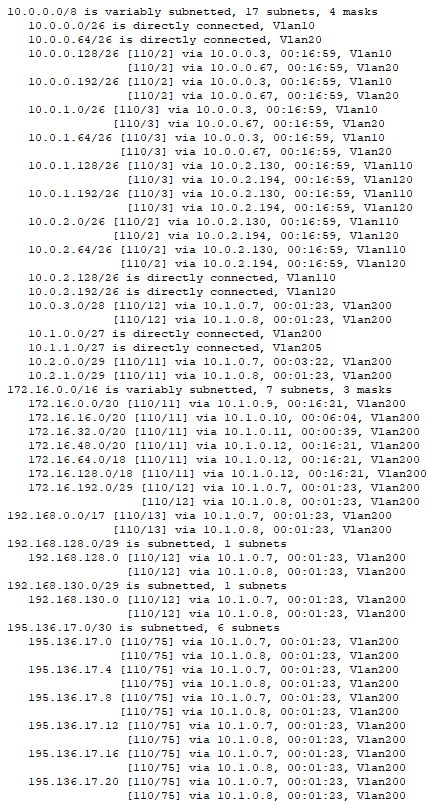
\includegraphics[width=0.5\textwidth]{Imágenes/OSPF Distr.png}
    \caption{OSPF en Switches de Distribución en Hospital Son Espases}
\end{figure}

\section{Validación DHCP}\label{anexo:Pruebadhcp}
A continuación se muestran algunas imágenes que corroboran que el protocolo DHCP está correctamente configurado y asigna direcciones IPs dinámicas a los dispositivos de la red.
\subsection{Dirección IP Dinámica en PC de Recursos Humanos}
\begin{figure}[H]
    \centering
    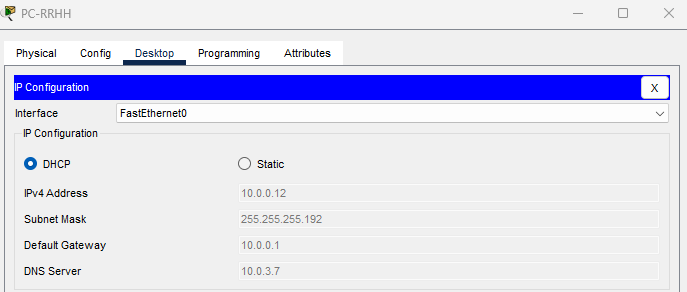
\includegraphics[width=0.5\textwidth]{Imágenes/DHCP-PC-RRHH.png}
    \caption{Dirección IP Dinámica en PC de Recursos Humanos}
\end{figure}
\subsection{Dirección IP Dinámica en PC de Admisión}
\begin{figure}[H]
    \centering
    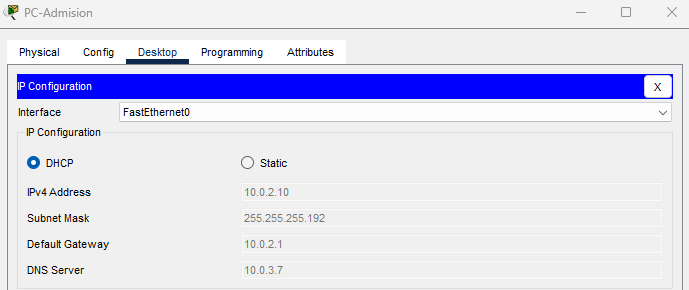
\includegraphics[width=0.5\textwidth]{Imágenes/DHCP-PC-Admision.png}
    \caption{Dirección IP Dinámica en PC de Admisión}
\end{figure}

\section{Validación NAT}
A continuación se muestran las traducciones de direcciones IPs hechas por el servicio NAT, que permiten la conectividad entre los dispositivos internos con Internet y viceversa.
\subsection{Traducción IPs hacia Internet}\label{anexo:haciaInt}
\begin{figure}[H]
    \centering
    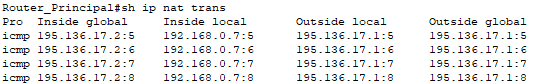
\includegraphics[width=0.5\textwidth]{Imágenes/natHaciaInternet.png}
    \caption{Traducción IPs hacia Internet}
\end{figure}
\subsection{Traducción IPs desde Internet}\label{anexo:desdeInt}
\begin{figure}[H]
    \centering
    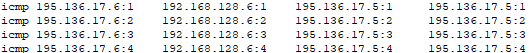
\includegraphics[width=0.5\textwidth]{Imágenes/natdesdeIntenret.png}
    \caption{Traducción IPs desde Internet}
\end{figure}

\section{Validación SSH}\label{anexo:pruebaSSH}
A continuación se muestra la imágen de la consola, donde se ve la conexión realizada mediante SSH a un dispositivo de red del hospital.
\begin{figure}[H]
    \centering
    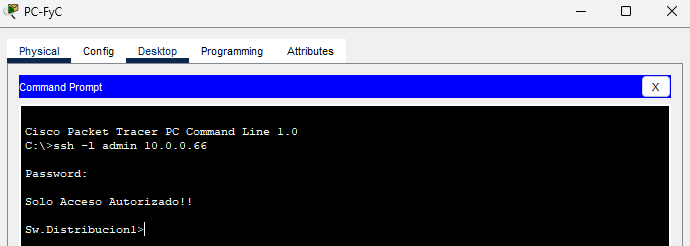
\includegraphics[width=0.5\textwidth]{Imágenes/ssh.png}
    \caption{Conexión Remota mediante SSH a Switch de Distribución 1}
\end{figure}

\section{Validación Autenticación en Dispositivos de Red}\label{anexo:pruebaAutent}
A continuación se muestra la imágen de la consola, donde se ve la autenticación realizada para poder acceder al switch de distribución 2.
\begin{figure}[H]
    \centering
    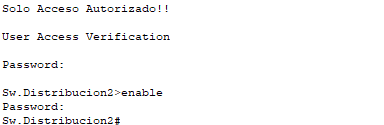
\includegraphics[width=0.5\textwidth]{Imágenes/Autent.png}
    \caption{Autenticación en Switch de Distribución 2}
\end{figure}

\section{Validación VPN IPSec}\label{anexo:pruebavpn}
A continuación se muestra la imágen de la consola, donde se ve la salida dada al insertar el comando "show crypto ipsec sa".
\begin{figure}[H]
    \centering
    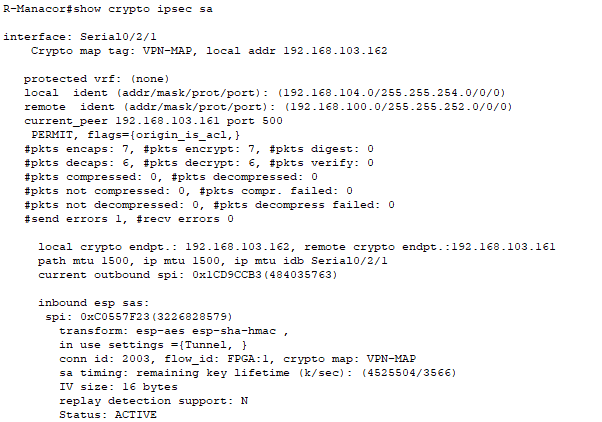
\includegraphics[width=0.5\textwidth]{Imágenes/vpn.png}
    \caption{Salida por consola de show crypto ipsec sa}
\end{figure}

\section{Validación DHCP Snooping}
\subsection{Interfaces en Modo Trusted}\label{anexo:pruebasnoo1}
A continuación se muestra la imágen de la consola, donde se ve la salida dada al insertar el comando "show ip dhcp snooping".
\begin{figure}[H]
    \centering
    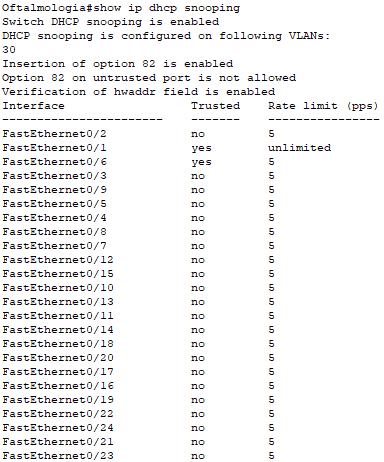
\includegraphics[width=0.5\textwidth]{Imágenes/dhcpsnooping.png}
    \caption{Salida por consola de show ip dhcp snooping}
\end{figure}

\subsection{Tabla de IPs}\label{anexo:pruebasnoo2}
A continuación se muestra la imágen de la consola, donde se ve la salida dada al insertar el comando "show ip dhcp snooping binding".
\begin{figure}[H]
    \centering
    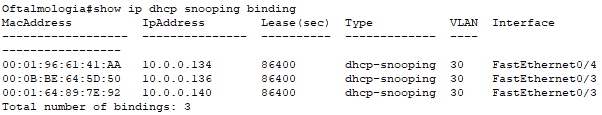
\includegraphics[width=0.5\textwidth]{Imágenes/snooping2.png}
    \caption{Salida por consola de show ip dhcp snooping binding}
\end{figure}

\section{Validación Conectividad}
\subsection{Conectividad Dispositivos Internos con Internet}\label{anexo:pruebaInt-Inter}
A continuación se muestra la imágen de la consola, donde se ve la salida dada al realizar el ping desde un PC de la red interna a la puerta de enlace del ISP 1 (Internet).
\begin{figure}[H]
    \centering
    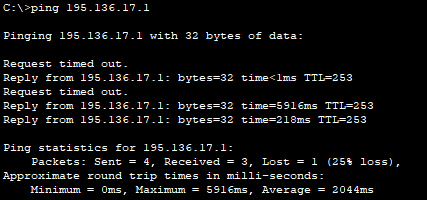
\includegraphics[width=0.5\textwidth]{Imágenes/inv-internet.png}
    \caption{Conectividad Dispositivos Internos con Internet}
\end{figure}
\subsection{Conectividad Dispositivos Invitados con Internet}\label{anexo:pruebaInv-Inter}
A continuación se muestra la imágen de la consola, donde se ve la salida dada al realizar el ping desde el portátil de la red de invitados a la puerta de enlace del ISP 1 (Internet).
\begin{figure}[H]
    \centering
    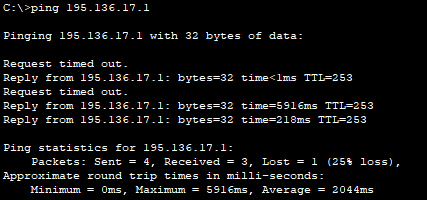
\includegraphics[width=0.5\textwidth]{Imágenes/inv-internet.png}
    \caption{Conectividad Dispositivos Invitados con Internet}
\end{figure}
\subsection{Conectividad Internet con Servidor Web}\label{anexo:pruebaInter-Serv}
A continuación se muestra la imágen de la consola, donde se ve la salida dada al realizar el ping desde la peurta de enlace del ISP 1 (Internet) al servidor web del hospital.
\begin{figure}[H]
    \centering
    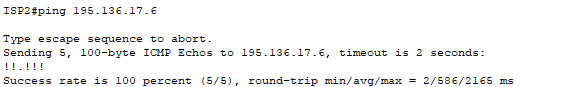
\includegraphics[width=0.5\textwidth]{Imágenes/inter-serv.png}
    \caption{Conectividad Internet con Servidor Web}
\end{figure}

\section{Validación ACLs Bloqueantes}
\subsection{Bloqueo entre Dispositivo Administrativo con Dispositivo IoMT}\label{anexo:blockadmin-iomt}
A continuación se muestra la imágen de la consola, donde se ve la salida dada al realizar el ping entre un dispositivo administrativo con un dispositivo IoMT.
\begin{figure}[H]
    \centering
    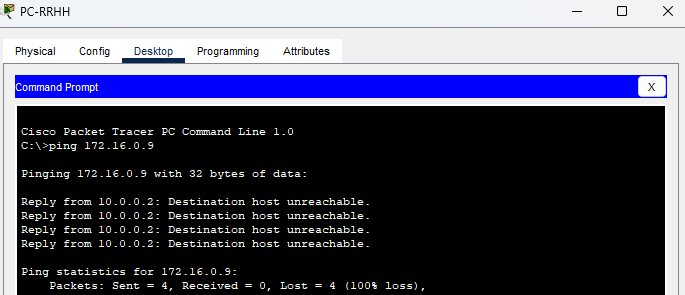
\includegraphics[width=0.5\textwidth]{Imágenes/BlockAdmin-Iomt.png}
    \caption{Bloqueo entre Dispositivo Administrativo con Dispositivo IoMT}
\end{figure}
\subsection{Bloqueo entre Dispositivo Administrativo con Dispositivo Médico}\label{anexo:blockadmin-med}
A continuación se muestra la imágen de la consola, donde se ve la salida dada al realizar el ping entre un dispositivo administrativo con un dispositivo médico.
\begin{figure}[H]
    \centering
    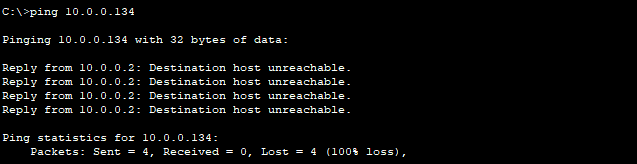
\includegraphics[width=0.5\textwidth]{Imágenes/blockadmin-medico.png}
    \caption{Bloqueo entre Dispositivo Administrativo con Dispositivo Médico}
\end{figure}
\subsection{Bloqueo entre Dispositivo Administrativo con Dispositivo de la UCI}\label{anexo:blockadmin-uci}
A continuación se muestra la imágen de la consola, donde se ve la salida dada al realizar el ping entre un dispositivo administrativo con un dispositivo de la UCI.
\begin{figure}[H]
    \centering
    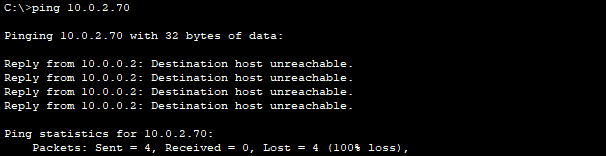
\includegraphics[width=0.5\textwidth]{Imágenes/blockadmin-uci.png}
    \caption{Bloqueo entre Dispositivo Administrativo con Dispositivo de la UCI}
\end{figure}
\subsection{Bloqueo entre Dispositivo Invitado con Dispositivo Interno}\label{anexo:blockinv-int}
A continuación se muestra la imágen de la consola, donde se ve la salida dada al realizar el ping entre un dispositivo invitado con un dispositivo interno.
\begin{figure}[H]
    \centering
    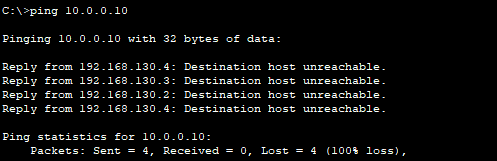
\includegraphics[width=0.5\textwidth]{Imágenes/blockinv-int.png}
    \caption{Bloqueo entre Dispositivo Invitado con Dispositivo Interno}
\end{figure}
\subsection{Bloqueo entre Dispositivo Invitado con Dispositivo IoMT}\label{anexo:blockinv-iomt}
A continuación se muestra la imágen de la consola, donde se ve la salida dada al realizar el ping entre un dispositivo invitado con un dispositivo IoMT.
\begin{figure}[H]
    \centering
    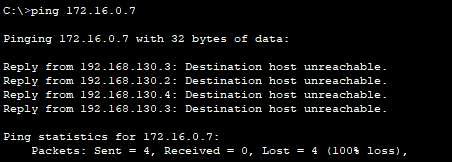
\includegraphics[width=0.5\textwidth]{Imágenes/blockinv-iomt.png}
    \caption{Bloqueo entre Dispositivo Invitado con Dispositivo IoMT}
\end{figure}
\subsection{Bloqueo entre Dispositivo No Autorizado con Servidor de Archivos}\label{anexo:blocknoaut-serv}
A continuación se muestra la imágen de la consola, donde se ve la salida dada al realizar el ping entre un dispositivo invitado con un dispositivo IoMT.
\begin{figure}[H]
    \centering
    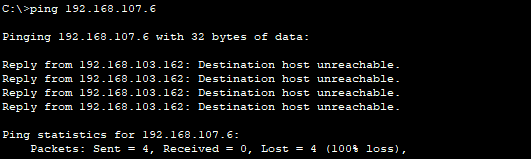
\includegraphics[width=0.5\textwidth]{Imágenes/blocknoaut-serv.png}
    \caption{Bloqueo entre Dispositivo No Autorizado con Servidor de Archivos}
\end{figure}

\section{Validación ACLs Permisivas}
\subsection{Conectividad entre Dispositivo Médico con Dispositivo UCI}\label{anexo:permmed-uci}
A continuación se muestra la imágen de la consola, donde se ve la salida dada al realizar el ping entre un dispositivo médico con un dispositivo de la UCI.
\begin{figure}[H]
    \centering
    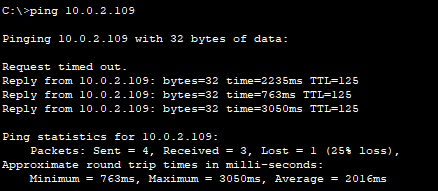
\includegraphics[width=0.5\textwidth]{Imágenes/permmed-uci.png}
    \caption{Conectividad entre Dispositivo Médico con Dispositivo UCI}
\end{figure}
\subsection{Conectividad entre Dispositivo Médico con Dispositivo IoMT Tipo 1}\label{anexo:permmed-tipo1}
A continuación se muestra la imágen de la consola, donde se ve la salida dada al realizar el ping entre un dispositivo médico con un dispositivo IoMT tipo 1.
\begin{figure}[H]
    \centering
    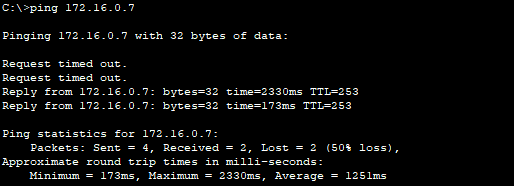
\includegraphics[width=0.5\textwidth]{Imágenes/permmed-tipo1.png}
    \caption{Conectividad entre Dispositivo Médico con Dispositivo IoMT Tipo 1}
\end{figure}
\subsection{Conectividad entre Dispositivo de la UCI con Dispositivo IoMT Tipo 2}\label{anexo:permuci-tipo2}
A continuación se muestra la imágen de la consola, donde se ve la salida dada al realizar el ping entre un dispositivo de la UCI con un dispositivo IoMT tipo 2.
\begin{figure}[H]
    \centering
    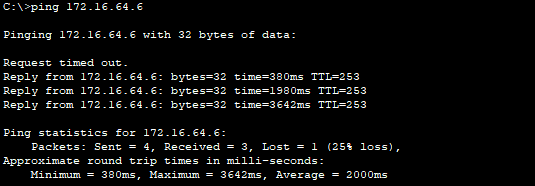
\includegraphics[width=0.5\textwidth]{Imágenes/permuci-tipo2.png}
    \caption{Conectividad entre Dispositivo de la UCI con Dispositivo IoMT Tipo 2}
\end{figure}
\subsection{Conectividad entre Dispositivo Autorizado de la UCI con Dispositivo IoMT Tipo 3}\label{anexo:permuci-tipo3}
A continuación se muestra la imágen de la consola, donde se ve la salida dada al realizar el ping entre el dispositivo autorizado de la UCI con un dispositivo IoMT tipo 3.
\begin{figure}[H]
    \centering
    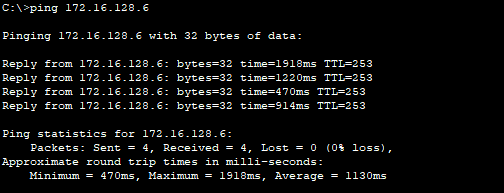
\includegraphics[width=0.5\textwidth]{Imágenes/permuci-tipo3.png}
    \caption{Conectividad entre Dispositivo Autorizado de la UCI con Dispositivo IoMT Tipo 3}
\end{figure}
\subsection{Conectividad PC Autorizado de IT con Servidor de Archivos}\label{anexo:permit-serv}
A continuación se muestra la imágen de la consola, donde se ve la salida dada al realizar el ping entre el PC de IT de Son Espases con el servidor de archivos del hospital de Manacor.
\begin{figure}[H]
    \centering
    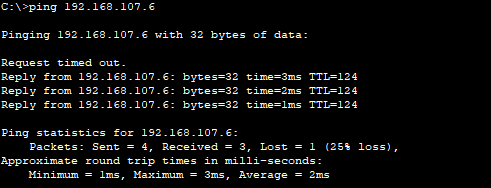
\includegraphics[width=0.5\textwidth]{Imágenes/permaut-serv.png}
    \caption{Conectividad PC Autorizado de IT con Servidor de Archivos}
\end{figure}

\section{Validación HSRP}
\subsection{HSRP en Routers}\label{anexo:pruebahsrprou}
A continuación se muestran las imágenes del estado del HSRP de los tres routers, antes de la caída del router principal y después de la caída del router principal.
\begin{figure}[H]
    \centering
    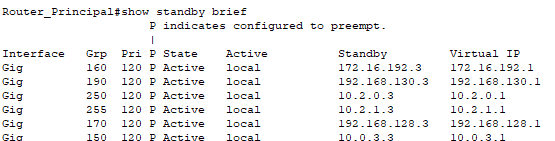
\includegraphics[width=0.5\textwidth]{Imágenes/RprincipalAntes.png}
    \caption{Router Principal Antes}
\end{figure}
\begin{figure}[H]
    \centering
    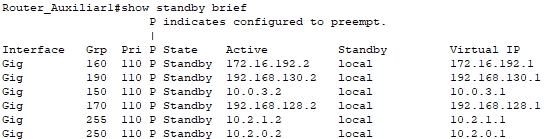
\includegraphics[width=0.5\textwidth]{Imágenes/Rauxiliar1Antes.png}
    \caption{Router Auxiliar 1 Antes}
\end{figure}
\begin{figure}[H]
    \centering
    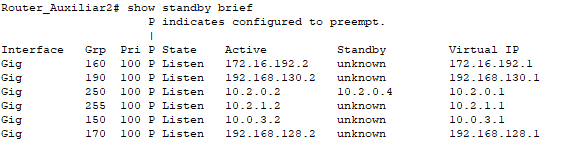
\includegraphics[width=0.5\textwidth]{Imágenes/Rauxiliar2Antes.png}
    \caption{Router Auxiliar 2 Antes}
\end{figure}
\begin{figure}[H]
    \centering
    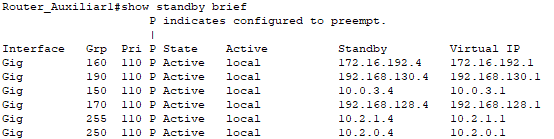
\includegraphics[width=0.5\textwidth]{Imágenes/Rauxiliar1Desp.png}
    \caption{Router Auxiliar 1 Después}
\end{figure}
\begin{figure}[H]
    \centering
    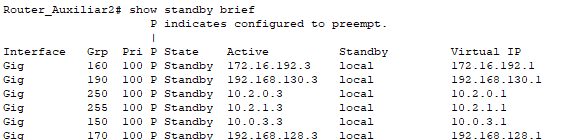
\includegraphics[width=0.5\textwidth]{Imágenes/Rauxiliar2depsues.png}
    \caption{Router Auxiliar 2 Después}
\end{figure}
\subsection{HSRP en Switches}\label{anexo:pruebahsrpsw}
A continuación se muestra las imágenes del estado del HSRP de los dos switches, antes de la caída del switch principal y después de la caída del switch principal.
\begin{figure}[H]
    \centering
    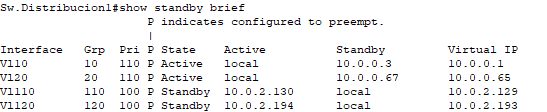
\includegraphics[width=0.5\textwidth]{Imágenes/Sw1Antes.png}
    \caption{Switch Principal Antes}
\end{figure}
\begin{figure}[H]
    \centering
    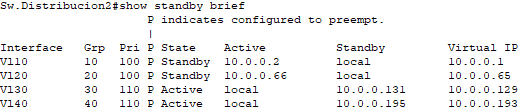
\includegraphics[width=0.5\textwidth]{Imágenes/Sw2Antes.png}
    \caption{Switch Auxiliar Antes}
\end{figure}
\begin{figure}[H]
    \centering
    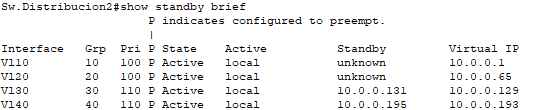
\includegraphics[width=0.5\textwidth]{Imágenes/Sw2Deps.png}
    \caption{Switch Auxiliar Después}
\end{figure}
\section{Validación EtherChannel}\label{anexo:pruebaether}
A continuación se muestra las imágenes del estado del EtherChannel de los dos switches, antes de la caída de un enlace redundante y después de la caída de un enlace redundante.
\begin{figure}[H]
    \centering
    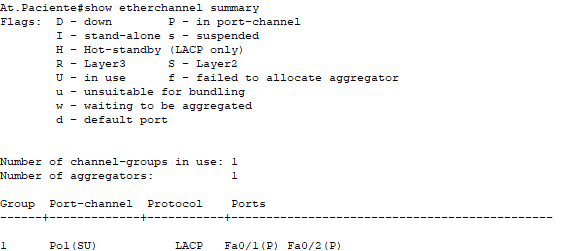
\includegraphics[width=0.5\textwidth]{Imágenes/SwAccAntes.png}
    \caption{Switch Acceso Antes}
\end{figure}
\begin{figure}[H]
    \centering
    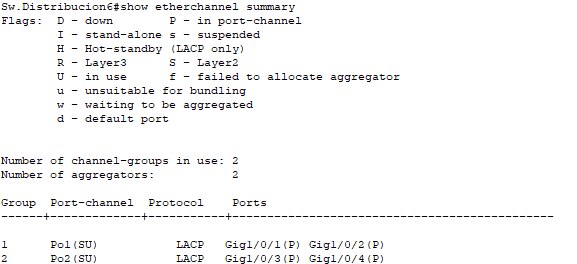
\includegraphics[width=0.5\textwidth]{Imágenes/SwDistrAntes.png}
    \caption{Switch Distribución Antes}
\end{figure}
\begin{figure}[H]
    \centering
    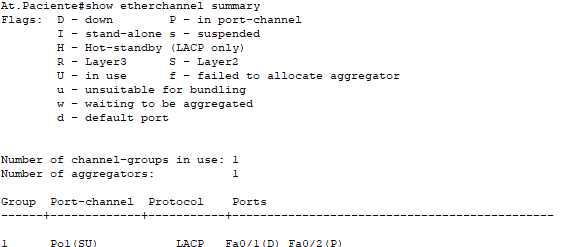
\includegraphics[width=0.5\textwidth]{Imágenes/SwAccDesp.png}
    \caption{Switch Acceso Después}
\end{figure}
\begin{figure}[H]
    \centering
    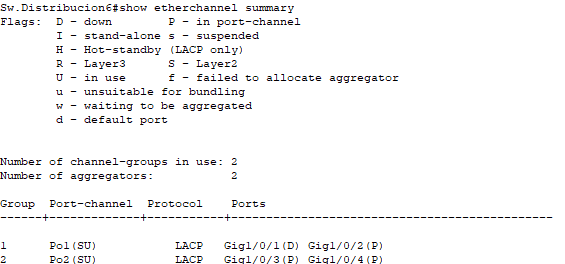
\includegraphics[width=0.5\textwidth]{Imágenes/SwDistrDesp.png}
    \caption{Switch Distribución Después}
\end{figure}
\section{Validación Subred Interconexión}\label{anexo:pruebasubrinter}

\section{Validación OSPF en Red Interconexión entre Hospitales}\label{anexo:ospfinter}
\begin{figure}[H]
    \centering
    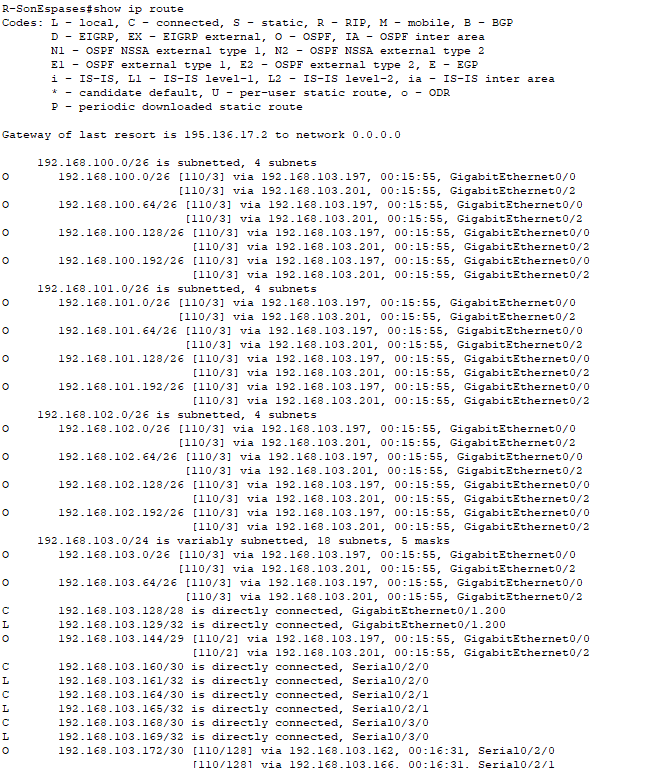
\includegraphics[width=0.5\textwidth]{Imágenes/ospf1.png}
    \caption{Validación OSPF en Red Interconexión entre Hospitales Parte 1}
\end{figure}
\begin{figure}[H]
    \centering
    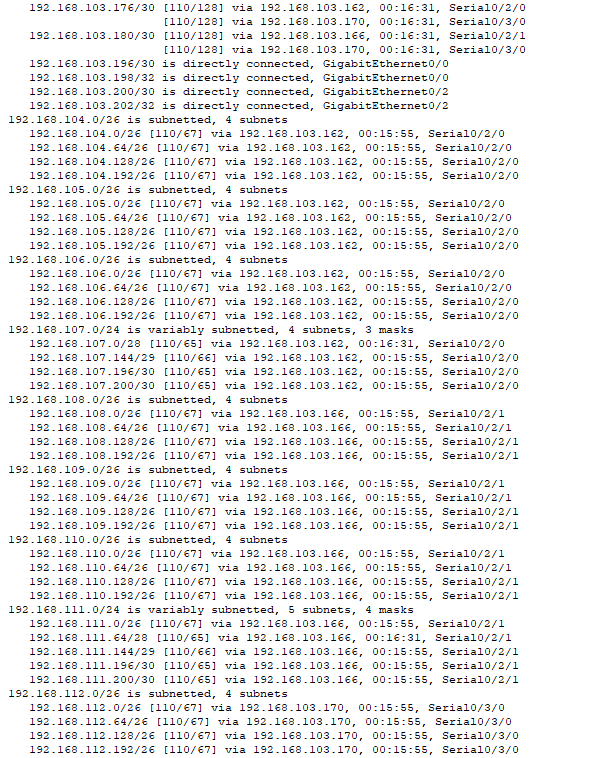
\includegraphics[width=0.5\textwidth]{Imágenes/ospf2.png}
    \caption{Validación OSPF en Red Interconexión entre Hospitales Parte 2}
    \label{fig:interconexion}
\end{figure}
\begin{figure}[H]
    \centering
    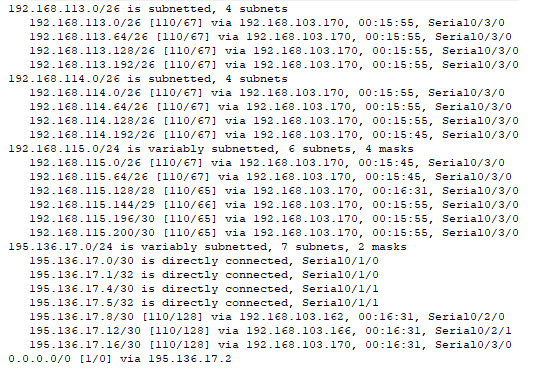
\includegraphics[width=0.5\textwidth]{Imágenes/ospf3.png}
    \caption{Validación OSPF en Red Interconexión entre Hospitales Parte 3}
    \label{fig:interconexion}
\end{figure}

\section{Red Completa del Hospital Son Espases}\label{anexo:redcompletasonespas}
\begin{figure}[H]
    \centering
    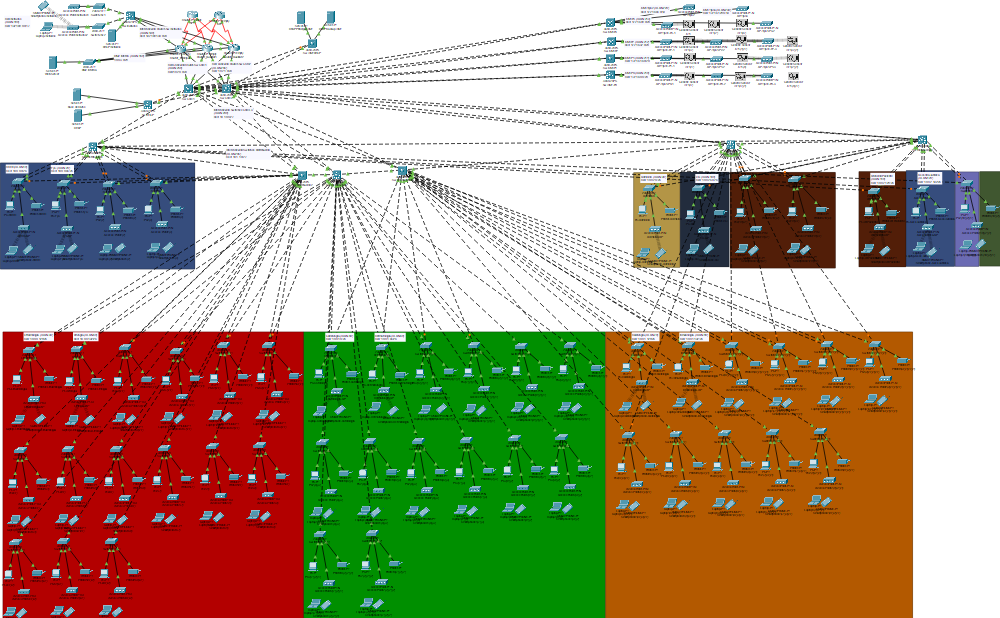
\includegraphics[width=\paperwidth, height=\paperheight, keepaspectratio, angle=270]{Imágenes/RedSonEspases.png}
    \caption{Red Completa del Hospital Son Espases}
    \label{fig:SonEspases}
\end{figure}
\section{Red Completa de Interconexión entre Hospitales}\label{anexo:redcompletahosp}
\begin{figure}[H]
    \centering
    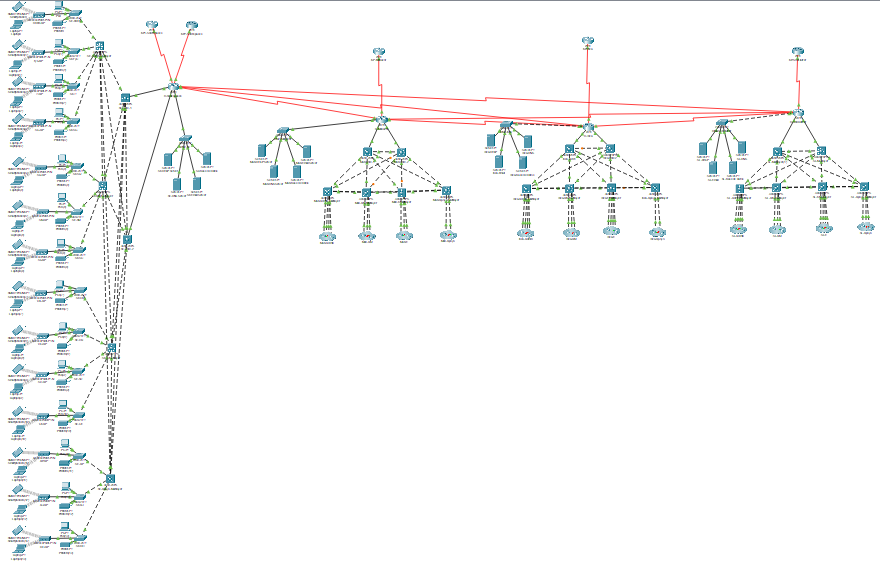
\includegraphics[width=\paperwidth, height=\paperheight, keepaspectratio, angle=270]{Imágenes/redInterocnexion.png}
    \caption{Red Completa de Interconexión entre Hospitales}
    \label{fig:interconexion}
\end{figure}

 

% En aquest cas sols hi ha un fitxer d'annexos,
% però podeu afegir tants \include com calgui. 

%%%%%%% Fi apèndix 

% No toqueu la línia següent 
\backmatter

% La comanda següent defineix l'estil bibliogràfic
\bibliographystyle{IEEEtran}

% La comanda següent defineix el fitxer que
% conté les referències bibliogràfiques.
% En aquest cas és el fitxer Bibliografia.bib
\bibliography{Bibliografia} 

\end{document}